\documentclass[letterpaper,12pt,oneside]{book}
\usepackage[top=1in, left=1in, right=1in, bottom=1in]{geometry}
%-----------------------__--------
%https://es.overleaf.com/project/642e50d937469ff17340bdc4
% Tesis UNAM https://tex.stackexchange.com/questions/234265/unam-thesis-title-page-portada-tesis-unam

%\usepackage{parskip} % Add the parskip package


\usepackage{setspace} % Add the setspace package
\setstretch{1.5} % Set line spacing to double

\usepackage{pdfpages}
\usepackage{lipsum}

\usepackage[T1]{fontenc}
\usepackage[utf8]{inputenc}
\usepackage[spanish,es-nodecimaldot,es-tabla]{babel}

\usepackage{graphicx}
\usepackage{float}
\usepackage{tikz}
\usepackage{setspace}

%% para codigos
\usepackage{listings}


%Subfiguras
\usepackage{caption}
\usepackage{subcaption}

% Para referencias 
\usepackage{hyperref}
\usepackage{apacite}
\usepackage{url}

%\addbibresource{CARDIAC}
%%% To make that images appear at the top of the page
	\makeatletter
	\setlength{\@fptop}{0pt}
	\makeatother
	%%%
\title{E-CARDIAC: La evolución hacia un modelo concurrente y paralelo}

\begin{document}
	\frontmatter
	\pagestyle{plain} % Set page style to "plain" for the front matter
	%\maketitle

    \includepdf{media/cover.pdf}

%---------------------------------
\chapter*{}
\begin{flushright}%
  \emph{``These are fast-moving times, and those who make no effort to understand computers may very well get left behind''}
  
  
  - David W. Hagelbarger, 1968
  %%\thispagestyle{empty}
\end{flushright}

\chapter*{Agradecimientos}
%\spacing{1.5}%\doublespacing

\chapter*{Abstract}

\chapter{Introducción}

	Hoy en día tenemos multitud de aparatos electrónicos que suelen ser llamados computadoras; celulares, laptops, tabletas, relojes inteligentes, y un sin fin más. 
	Estos aparatos suelen ser llamados así dado que son capaces de resolver operaciones aritméticas y lógicas, guardar datos, procesarlos, y recibir instrucciones del 
	usuario, esto siguiendo la definición
	que recoge el diccionario de Oxford\footnote{Usado como fuente dado que la lengua franca de la computación es el inglés.} tiene sentido,
	pero si analizamos más detalladamente el termino ``computadora''  notaremos que el origen de la palabra es anterior a las computadoras
	tal cual las conocemos hoy día, por ejemplo antes de 1950 la palabra ``computadora''  era referida comúnmente a mujeres
	que trabajaban en la NASA y realizaban cálculos manuales, como lo describe el blog \cite{nasa_who_2020} de la NASA dedicado a Katherine Johnson, destacada "computadora humana" que aún con el machismo que se vivía en la época logro ser ampliamente reconocida y ver como esa misma palabra que la había descrito a ella en el pasado
	era usada para describir a potentes máquinas electrónicas de cálculo.

	Si viajamos al pasado remoto notaremos que desde muy temprana edad se buscaba disminuir las tareas repetitivas para los humanos, pasando por el ábaco
	en muchas culturas, hasta máquinas más complejas a partir del siglo XVI, o con técnicas como los logaritmos o las tablas de multiplicar. Esta búsqueda junto
	al desarrollo de otras tecnologías en paralelo permitió la creación de máquinas que podían ir más de allá que automatizar cálculos,
	máquinas de propósito general, que pudieran cambiar su funcionamiento de acuerdo a la interacción con el usuario y resolver
	una multitud de problemas nunca antes pensada\cite{ifrah_universal_2001}. En tal estudio del pasado nos daremos cuenta de la cantidad de sucesos y desarrollos que tuvieron 
	que acontecer para llegar desde automatizaciones muy particulares de cálculos aritméticos hasta las computadoras que conocemos hoy en día. 
	%Sinonimos?
	%%https://www.smithsonianmag.com/science-nature/history-human-computers-180972202/

	Aunque tenemos una remota idea de lo compleja que fue la invención de la computadora no se suele conocer ni siquiera superficialmente
	la forma en que funciona una computadora, el como podemos enviar mensajes de texto mientras escuchamos una canción, si acaso hay algún programa que ejecuta a los 
	demás programas que utilizamos, o incluso si hay un programa que da inicio a todos los procesos de una computadora. Por que al final son temas complejos
	que requieren su tiempo de estudio, lo que no puede suceder es que profesionales o estudiantes de carreras afines a la computación no conozcan estos detalles, y
	es que muchas veces se da por sentado que es conocimiento general y en especializaciones como desarrollo web o arquitectura de software(solo como ejemplo) no se le suele
	prestar mucha atención. Sin embargo el conocimiento, al menos básico, del funcionamiento interno de una computadora es fundamental para saber
	como explotar de mejor manera los recursos de las máquinas que estás utilizando en cualquier disciplina que te desempeñes. Aunado a esto conocer la historia
	es otro punto fundamental,
	te permitirá saber la razón por la cuál ciertos aspectos de las computadoras no han cambiado en 80 años y el por que otros han cambiado o evolucionado
	de manera tan vertiginosa en los últimos años, preparándote también para el futuro y dando el reconocimiento que se merecen a aquellas personas que
	con sus aportes contribuyeron a la revolución que trajo consigo la invención de la computadora.
	
	Estos pensamientos surgieron a lo largo de mi carrera universitaria, pero fue al final de está que decidí abordarlos y empezar este proyecto de investigación
	con el fin de centrar en un mismo texto un repaso histórico de la computación acompañado de una descripción didáctica del funcionamiento de las computadoras
	y su evolución a lo largo de la historia. Pero como la intención tampoco es crear un manual completo de las computadoras y su historia el repaso
	se centrará principalmente en el origen de las computadoras y como funciona, groso modo, una computadora actual. Para esto último me apoyaré
	de \textit{CARDIAC(CARDboard Illustrative Aid to Computation)}, un modelo de computación 
	desarrollado por Bell Labs de la mano de David W. Hagelbarger y Saul Fingerman en 1968\cite{hegelbarger_instruction_1968} con la intención, precisamente,
	de hacer más fácil de entender a los alumnos de aquel entonces el como funcionaba una computadora. No fue el único intento, otro que se debe mencionar es
	\textit{Little Man Computer(LMC)} creada por Stuart Madnick y Jhon Donovan del MIT en los años 60, que con un reducido conjunto de instrucciones permitía a los estudiantes 
	probar la ejecución de programas como si estuvieran en una computadora real. Ambos modelos mencionados en \cite{mark_jones_lorenzo_paper_2017}, que
	no puedo dejar de mencionar como una de las lecturas que más me inspiraron en la escritura de está tesis.
	
	El reto con \textit{CARDIAC(CARDboard Illustrative Aid to Computation)} es que fue creado en 1968, por lo que la concurrencia, el paralelismo o
	la inclusión de un sistema operativo no pasaban por la mente de sus creadores dado que aún no eran tan relevantes en la industria estos términos. Así que
	para poder llegar a las computadoras actuales concurrentes, paralelas y con un sistema operativo decidí diseñar una ``evolución'' de CARDIAC que permita
	entender estos conceptos de una forma didáctica, aprovechando las ventajas un modelo que abstrae un sistema complejo en los componentes principales
	que se quieren dar a entender. Aprovechando el contexto histórico se darán las razones por las que cuales cada paso en la evolución de las
	computadoras fue necesario e incluso aveces imparable, manteniendo la atención principalmente en estos 3 conceptos sin desviar la atención en
	muchos otros avances, especialmente de hardware, que son fundamentales pero no el tema central de está tesis.
	 
	Es claro que en todo esté tiempo surgieron otros modelos con la intención de ayudar a los estudiantes a entender el funcionamiento de una computadora, algunos
	de ellos que debo mencionar por su relación con CARDIAC son : \textit{MARIE(Machine Architecture that is Really Intuitive and Easy)} un muy interesante 
	desarrollo presentado en \cite{null_essentials_2003} que se enfoca en los aspectos básicos del funcionamiento al igual que CARDIAC, otro es un desarrollo
	hecho en Argentina alrededor de los años 80 llamado \textit{TIMBA(Terrible Imbecile Machine for Boring Algorithms)} que incluso tenía un lenguaje de programación
	como nos describe el articulo \cite{alvaro_frias_retruco_2022} centrado en dicho lenguaje, por último he de mencionar un desarrollo
	mostrado en el articulo \cite{ajdari_design_2012} que presenta a \textit{Abu-Reiah} un procesador de 8 bits simplificado que incluye un simulador 
	gráfico
	para ayudar a los estudiantes de arquitectura de computación. Mi intención con las mejoras a CARDIAC no es suplir ninguno de los trabajos antes mencionados,
	sino más bien complementarlos con un desarrollo histórico que presente de forma clara, concisa y didáctica 4 aspectos fundamentales en la evolución
	de la computación, la concurrencia, el paralelismo, el uso del sistema operativo y la programación.
	
	
	Más allá del recorrido en la construcción y diseño de modelos ``evolucionados'' de CARDIAC el texto se verá acompañado,
	tal como la clásica CARDIAC distribuida por Bell Labs, con un ``kit'' que incluye un programa que contendrá tres máquinas virtuales\footnote{La emulación de una
	maquina física que virtualiza cada uno de sus componentes, incluido el hardware.}, uno para cada
	modelo de CARDIAC, con la diferencia de que estas máquinas virtuales ya no serán en papel, sino interfaces gráficas para uso en computadoras de escritorio con la idea de 
	que sea fácil para el estudiante
	entender la teoría y practicarla, poder ver como se van ejecutando los programas que ya en una versión paralela o concurrente sería un poco más difícil de ver con una 
	computadora de papel dada la cantidad de información que se tiene que almacenar.
	


\tableofcontents
\listoffigures

\mainmatter

\chapter{Historia de la computación} 


	\section{Breve recorrido por el pasado}
		\subsection{Antecedentes}
		% máquinas parecidas a las computadoras, que no lo son
		
		Desde que los humanos empezamos a hacer cálculos en el sentido de sumar o restar cantidades representadas por números hemos necesitado de herramientas
		que nos apoyen en la resolución del calculo, y entre más complejo el calculo necesitamos herramientas más complejas. Las
		primeras herramientas para apoyarnos en esto fueron fueron formas de representar los números de formas abstractas, una evolución continua en la abstracción
		de los números permitió a algunas civilizaciones crear artefactos con más potencia de cálculo, como el \textbf{ábaco}; el cuál se ha encontrado
		en diversas civilizaciones en diferentes épocas de la humanidad, el más antiguo del que se tiene registro es el inventado por la civilización
		Sumeria alrededor del año 2700 A.C. Otras civilizaciones siguieron sus desarrollos de manera independiente no solo para llegar a un artefacto
		similar al ábaco, sino para evolucionar su forma de hacer cálculos y la complejidad de estos, como es el caso de los griegos, una de las civilizaciones
		más importantes de nuestro mundo, que dieron un gran aporte al desarrollo de la matemática, tanto que muchos de sus descubrimientos siguen siendo
		enseñados hoy en día, y que por supuesto aumentaron la complejidad en los cálculos aritméticos. Está evolución paralela entre la aritmética que teníamos como humanidad 
		y las herramientas para solucionar esos cálculos
		fue construyendo un camino, o quizá varios, que en ciertos puntos confluyeron en la creación del siguiente hito en la simplificación de la resolución
		de cálculos, la \textbf{calculadora}, y de la misma forma nos llevarían hasta la creación de la primera \textbf{computadora} digital, que posteriormente se convertiría
		en algo mucho más grande y completo de lo que quizá se imaginaba en su creación\cite{ifrah_universal_2001}.
		
		%% Ser más claro para la definición de lo que ingresa a la computadora
		Siguiendo la mencionada evolución es importante mencionar la época en la que surgieron las primeras calculadoras mecánicas, así
		como ciertas herramientas para minimizar el esfuerzo en los cálculos realizados por los usuarios. Es el siglo 17 en Europa occidental,
		saliendo del renacimiento(europeo), en el cuál tienen necesidades más complejas en ciencias exactas y en problemas aplicados, los
		cálculos para la navegación y los astronómicos son ejemplos claros de ello. Por esa razón el descubrimiento de
		los logaritmos por parte de Jhon Napier en 1614 fue uno de los grandes avances en la forma de resolver problemas aritméticos,
		los logaritmos, groso modo, te permiten sustituir multiplicaciones por sumas, lo cuál significa una simplificación enorme
		en la resolución de estas operaciones\cite[p. 24]{oregan_brief_2012}. Pero aún así los cálculos seguían sin ser tan rápidos,
		por lo que se desarrollaron tablas de logaritmos ya calculados que hacían esté proceso más simple; otro avance importante en este
		tiempo fue el desarrollo de dispositivos mecánicos que permitían optimizar ciertos cálculos, \textit{The Gunter Scale} y \textit{The Slide Rule},
		creada la primera por Edmund Gunter y la segunda por William Oughtred como mejora a la primera, fueron dos dispositivos que
		ayudaban en la solución de operaciones aritméticas, de hecho \textit{The Slide Rule}(la regla de cálculo) siguió evolucionando a lo largo de los años para añadir más
		funcionalidades, como el uso de logaritmos, lo que la mantuvo vigente hasta hace relativamente poco tiempo(especialmente en áreas de ingeniería)\cite[p.24 y p. 96]{oregan_brief_2012}.				
		 Un poco más lejos llegarían Blaise Pascal y Wilhelm Gottfried Leibniz con sus inventos, que ya serían calculadoras en forma, Leibniz inventaría la
		\textit{Step Reackoner} o simplemente ``maquina de Leibniz'', que permitía hacer cálculos aritméticos, en el año de 1673, basada en \textit{The Pascaline} o
		\textit{Arithmetic Machine} creada por Pascal en 1642\cite[p.25]{oregan_brief_2012}.Ambas ya podían ser llamadas calculadoras funcionales, aunque ya desde muchos años 
		antes se venía pensando
		en un dispositivo como la calculadora, de hecho Leonardo Da Vinci  dejaría sus planos para construir un dispositivo de calculo(el cual no pudo construir), que
		ingenieros de la época moderna pudieron seguir para crearla\cite{california_state_university_historical_nodate}.
		Podemos notar que las inquietudes por automatizar operaciones estaban
		ya desde antes que la tecnología de su época les permitiera a los inventores llevar a cabo sus planes, pero que a pesar de esto las siguientes
		generaciones siguieron adelante con esas ideas, a veces independientemente y otras usando de base lo que ya existía de antes, para
		continuar con la innovación; este interesante patrón, dónde la teoría avanza más rápido que los desarrollos prácticos, lo veremos de nuevo en el futuro.
		%Slide rule en ingenieria
		
		Aunque las máquinas de Leibniz y Pascal eran calculadoras en forma, su replicación no era tan fácil y tampoco fueron muy populares, pero
		si hay una época dónde replicar máquinas para automatizar procesos va a estar en su auge esa es la \textbf{revolución industrial}. En
		1820 un francés llamado Charles Xavier Thomas de Colmar construyo el \textit{Arithmometer} basándose en la terminología de Leibniz, fue la primer
		calculadora en forma que se vendió masivamente, en los años sucesivos continuo recibiendo mejoras y al final fue toda una inspiración para una multitud de inventores 
		alrededor del mundo\cite[p. 127]{ifrah_universal_2001}.
		
		El antecesor directo de la computadora, y sucesor casi directo del ábaco no sólo había nacido, sino que ya había conseguido llegar a gran parte de
		la población, así que, si ya se había logrado el reto, ¿cuál era el siguiente? ¿hacerla más pequeña? si, más pequeña para que pudiera llegar a más personas,
		más veloz y que pudiera hacerse más fácil el uso para el usuario, al menos esa sería la respuesta general, ¿cual sería la de un visionario? Alguien
		que piensa más allá de las convenciones quizá pensaría un dispositivo que fuera capaz de ir más lejos. Y ese era Charles 
		Babbage,
		un reconocido matemático de su época, miembro fundador de la \textit{Royal Astronomical Society} en 1920, inventor, pionero en la investigación
		de operaciones, alguien muy distinguido en su época sin duda. Para el año de 1821 estaba diseñando su \textit{Differential Engine}, una maquina totalmente mecánica que
		en principio buscaba resolver el problema de precisión que tenían las calculadoras del momento, además de resolver funciones polinómicas de hasta
		grado 6. Lamentablemente no llegaría a ser producida por Charles, en parte por lo difícil(y costoso) que era en la época, y en parte por que Charles ya estaba pensando 
		en algo incluso más innovador; aún así la maquina se logro construir en 1853 por un par de ingenieros suecos que se basaron en los planes de Charles
		\cite[p.201]{oregan_brief_2012}.
		
		Lo que Charles ya estaba pensando, y de hecho en 1833, cuando se dio por terminada la construcción de la \textit{Differential Engine}(por que el maquinista que la 
		construía renuncio), estaba decidido a construir era la  \textit{Analytical Engine}, una maquina capaz de realizar cualquier tarea que pudiera
		ser expresada en notación algebraica  y que disminuía la interacción humana para realizar los cálculos. Era una maquina mucho más compleja, tendría un
		almacenamiento, y un procesador que Charles llamaba \textit{the mill} por que tenía la forma de un molino y era la parte que realizaba las operaciones; además
		contaría con elementos para la entrada y salida de datos usando la idea del \textit{telar de Jacquard}\footnote{ Un telar inventado por el francés Joseph-Marie-	Jacquard en 1804 para poder cambiar los patrones de los tejidos.}, que usaba tarjetas perforadas\footnote{Eran tarjetas de 
		cartón(usualmente) que tenían orificios con los que se representaban patrones, se continuaron usando por mucho tiempo en las computadoras digitales como podemos ver en 
		el vídeo: \emph{Punch Card Programming, \url{https://www.youtube.com/watch?v=KG2M4ttzBnY} }}
		para cambiar los patrones de diseños del telar, Charles pensó en usar estas tarjetas para representar números en ellas para realizar las operaciones
		de la maquina y de está forma podía hacer que su maquina fuese ``programable'', por que de hecho consideraba dos tipos de tarjetas:
		
		\begin{enumerate}
			\item Tarjetas de operación
			\item Tarjetas de datos
		\end{enumerate}
		
		Con está última idea de hecho se puede vislumbrar algo muy parecido a las computadoras con arquitectura Von Neumman, un procesador, almacenamiento interno,
		programas almacenados(en forma de tarjetas de operación y de datos)\cite[p.204]{oregan_brief_2012}. Es más en 1943 Lady Ada Lovelace, una matemática
		que estaba entusiasmada con el trabajo de Charles, realmente brillante, y que escribió un articulo al que 
		nombraría \textit{Notes} al final de una traducción que realizo de un trabajo
		del francés al inglés escrito por Luigi Manebra sobre la \textit{analytical engine}, en las cuales detalla el funcionamiento de la maquina, las cualidades que la 
		hacen diferente a las calculadoras de la época, y
		ejemplos de programas para cálculos realmente complejos como el calculo de los números de Bernoulli(de hecho esté se considera como
		el primer programa de la historia), por supuesto con una cercanía muy alta hacía Charles, como se deja ver en su correspondencia, lo que le permitió realizar un 	
		trabajo muy completo, esté articulo junto con las notas de Ada posteriormente sería publicado
		en al revista \textit{Scientific Memoir} bajo el titulo \textit{Sketch of the analytical engine invented by Charles Babbage}. De los elementos más valioso que nos 
		dejo,fueron por supuesto los programas y los detalles del funcionamiento de la maquina(junto a Manebra) que realizó, pero también su visión sobre el trabajo de 
		Charles, que era un tanto diferente a lo que el mismo consideraba, dado que 
		ella pensaba que la maquina podría actuar sobre otras algo más que números, si se creaban las relaciones correctas entre los números  como representación de algo 
		abstracto para fungir como símbolos se podrían realizar más tareas. Ada consideraba a la maquina analítica como algo muy lejano a las calculadoras de su época,
		y lo era en muchos sentidos, y aunque no fue construida en su tiempo al igual que su predecesora\footnote{Fue construida en 1991 por un equipo en el museo de ciencia de Londres usando los planos de Charles y es exhibida actualmente ahí, probando que Charles tenía razón.}, por sus aportes a la computación
		se le considera como la primer computadora(mecánica) de la historia\cite{eric_kim_ada_1999}.
		
		\begin{figure}
		    \centering
		    \includegraphics[scale = 0.6]{media/Historia/analyticalEngine1_sydbeypadua.jpg}
		    \caption{Fuente: Sydney Padua (2015), The Analytical Engine.}
	    	\label{fig:analytical_engine}
		\end{figure}
				
		En los años siguientes el avance fue continuo con estás máquinas calculadoras de propósito especifico que fueron mejorando con el paso del tiempo, se desarrollo
		por ejemplo una maquina de censos muy avanzada para su época por el fundador de la empresa hoy conocida como IBM. También la tecnología en general evolucionó,
		la era de la electricidad y lo electromecánico llegó a finales del siglo IX, el invento del tubo de vacío, y también
		avances teóricos que sucedieron, como el álgebra de Boole. Me parece importante hacer notar como no es una sucesión lineal de hechos o descubrimientos
		lo que llevaron a la creación de la computadora digital o de sus predecesoras, sino que el avance en muchas ramas de la ciencia, de la mecánica, y otras
		disciplinas fueron interactuando y creando descubrimientos revolucionarios para su época como lo hemos visto en esté capitulo y como
		se verá en los siguientes. En la siguiente sección analizaremos principalmente ese avance teórico que dio lugar a la evolución de las ``calculadoras'' mecánicas.
		
		% Usar automatas está bien?

		\clearpage		
		
		\subsection{Primeros autómatas}
		% Breve historia de como se fue desarrollando la computación desde los inicios hasta llegar a automatas(1950)
		
		Los avances tecnológicos en las máquinas que automatizan cálculos no pararon, e incluso mejoraron en el siglo 20 con la llegada de la electricidad
		y la electromecánica. Para el año 1913 el matemático Español Leonardo Torres Quevedo desarrollo su \textit{Artimómetro electromecánico}, evitando las
		dificultades que había tenido Babbage con ayuda de la electromecánica y con su gran ingenio pudo llevar a cabo este desarrollo que resolvía diversos
		problemas aritméticos y contaba con una maquina de escribir como entrada. Este no sería el único aporte
		a la computación de Quevedo, otro de los hechos por los que es conocido es por sentar las bases de la \textit{automática} en su \textit{Ensayo sobre automática}, 
		tomando
		la definición de autómata como ``maquina que imita la figura y los movimientos de un ser animado'' Quevedo desarrollo la idea centrado en las posibilidades
		de las máquinas como las calculadoras, pero que pudieran reconocer más objetos, más situaciones y en resolver problemas más difíciles, para así
		quitarles trabajos repetitivos a los humanos. El en su afán de demostrar que su teoría tenía sentido desarrollo un autómata llamado
		\textit{El Ajedrecista} que en su primera versión podía terminar un juego de ajedrez, es decir no podía jugar la partida completa,
		pero podía terminarla\cite{museo_torres_quevedo_ajedrecista_nodate,ifrah_universal_2001}.
		% Cambiar citas para incluir el ensayo de Leonardo Torres Quevedo
		
		Quevedo había lanzado preguntas muy interesantes en su ensayo acerca de los autómatas que se relacionan directamente con la computación, pues cuestiona
		las capacidades de una maquina para hacer algo más que lo que se lograba con una calculadora, aunque por las limitaciones tecnológicas estos cuestionamientos
		eran más teóricas que practicas. Pero, de hecho es justo en la teoría dónde se da el siguiente gran avance en la computación; motivados por \textit{los problemas
		de Hilbert}, una serie de problemas matemáticos que buscaban de dar más rigurosidad a las matemáticas desde el principio del siglo 20, Alan Turing
		y Alonzo Church comenzaron a trabajar por separado en resolver un problema muy particular, el famoso \textit{problema de la parada}, que sin entrar en mucho
		detalle trata sobre saber si todo problema matemático reproducible en un algoritmo puede ser resuelto, si una maquina que está ejecutando el algoritmo
		se detiene con seguridad siempre significa que si puede ser resuelto, siendo un algoritmo una lista de instrucciones ordenadas y finitas que permite solucionar un 
		problema. La resolución
		del problema es muy compleja y no es la idea del texto entrar en esos detalles, pero si dar a entender lo importante que fue para la computación su resolución
		y el trabajo teórico que se hizo.
		
		Se desarrollaron modelos teóricos de máquinas que podían ``computar'' en el sentido más clásico de la palabra, hacer cálculos. Turing trato de crear
		una maquina lo más general posible, de forma que cualquier problema que se pudiera computar en esa ``maquina de propósito general'', sea una calculadora
		o una maquina que resuelve polinomios, a tal maquina la llamo \textit{Maquina Universal de Turing} en su famoso articulo
		\textit{On computable numbers, with an application to the
		Entscheidungsprobkm}(Sobre números computables, con aplicación a el problema de la parada)\footnote{En 1936 se presenta la tesis de Alan Turing y Alonzo Church, con
		aproximaciones distintas a la solución del problema de la parada.}, dando también una definición rigurosa del concepto
		de algoritmo. Un modelo
		totalmente teórico, pero que mostraba todo el potencial de una maquina de propósito general que podía resolver cualquier problema que pudiese ser expresado
		como un algoritmo, pero que no podía resolver todos los problemas aritméticos, por que no hay suficientes algoritmos para representar todos los
		problemas que existen, así que la respuesta al problema de la parada es no, no se pueden resolver todos los problemas matemáticos en base
		a un algoritmo. De está forma se iba creando lo que posteriormente sería conocido como teoría de la computación, un estudio matemáticamente riguroso
		sobre las capacidades de las máquinas de computo que se subdivide en varias ramas, una que nos interesa es la \textit{teoría de la computabilidad}, que estudia
		que algoritmos puede computar una maquina, para llegar a establecer que ciertos problemas son no computables y por ende no son solubles por medio de
		ninguna computadora\cite[p. 272]{ifrah_universal_2001}.
		
		La forma de pensar sobre las máquinas ha evolucionado mucho a esté punto en la historia, la visión ahora es sobre una maquina que de soluciones a problemas que
		puedan ser descritos en forma de algoritmo, y ya no solo soluciones a problemas aritméticos o de funciones matemáticas. Turing y Church
		fueron dos nombres que dieron un salto gigante en está ciencia, que en ese momento aún no existía, de la teoría de la computación. En estos mismos años la evolución
		de en las máquinas continuaba, y en los siguientes años su expansión, causada también por el conflicto armado, no haría más que acelerarse.
		
		\clearpage		
		
		\subsection{Primeras computadoras}
		%1930-1945
		
		Es el momento de hablar de computadoras en forma, máquinas que ya se pueden considerar uniformemente como computadoras para la definición general
		que se tiene de estás. Repasaremos lo sucedido entre el año de 1930 y 1946 dónde por diversas causas, la madurez en el entendimiento de las
		máquinas de cálculo, de la electromecánica y la electricidad, así como necesidades de una mejora tecnológica para enfrentar una de las guerras
		más crueles que ha visto la humanidad, se dieron las condiciones para el desarrollo de la computación. En primera instancia
		como la evolución de las calculadoras, pero que se fue deformando hasta convertirse en más bien máquinas que resolvían problemas específicos.
		
		Como en está parte de la historia está centrada la discusión de cuál fue la primer computadora de la historia es necesario tener una definición
		más clara de lo que entendemos por computadora, y por que ciertas máquinas están en el limbo entre calculadoras o computadoras y otras
		ya son computadoras en un sentido más completo.Empecemos con la definición 
		del diccionario de Oxford, definición que uso dado que es entre Gran Bretaña y Estados Unidos que se da principalmente el desarrollo de las computadoras
		en sus inicios, y por tanto es su lengua franca:
		\begin{enumerate}
			  \item[] \emph{ Definición 1:} Una persona que hace cálculos, especialmente con una maquina de calcular.
			  \item[] \emph{ Definición 2:} Un dispositivo electrónico para guardar y procesar datos, típicamente en forma binaria, de acuerdo a las instrucciones
			  dadas en un programa(conjunto de instrucciones).
		\end{enumerate}
		
		La primera definición, que aún perdura, hace referencia principalmente al significado que tenía antes de 1940. Por que posteriormente, entre 1940 y 1950
		con la aparición de las máquinas electromecánicas o eléctricas se empezó a usar el termino con la connotación que tenemos de el hoy en día. Por ende
		la segunda definición nos interesa más, y que es acorde a muchos libros de computación, como  en \cite{goldstine_computer_1972} Goldstine nos dice lo siguiente 
		acerca de la computadora : ``Es un dispositivo electrónico que puede recibir un conjunto de instrucciones, o un programa,
		y entonces resolver este programa realizando varias operaciones matemáticas en datos numéricos '', a partir de estás definiciones podemos establecer
		4 características fundamentales en una computadora:
		
		\begin{enumerate}
			\item Dispositivo electrónico 
			\item Guarda datos
			\item Procesa datos
			\item Realiza operaciones a partir de un conjunto de instrucciones dadas por el usuario(Entendiendo programa como una forma de algoritmo)
		\end{enumerate}
		
		Todo lo que hace una calculadora lo hace, y con más capacidades, pero hay un punto importante para nuestro estudio, ¿que no sea un dispositivo electrónico es
		necesario para que una maquina que tiene las otras tres características	no sea una computadora? Realmente la mayoría de los autores lo manejan directamente
		como un dispositivo electrónico y no se involucran en la discusión de que es una computadora. Como veremos realmente un dispositivo mecánico o electromecánico
		puede cumplir con el resto de especificaciones, pero dado que su uso fue más bien en el nacimiento de la computación y quedo rápidamente sobrepasado
		por la potencia de los dispositivos electrónicos no se encuentra mucho problema en la definición dada por Goldstine.
		
		%% Pre - Guerra
		
		En está época hubo una gran explosión de desarrollos en cuanto a máquinas que automatizaban cálculos, desde
		aquellas que eran calculadoras muy potentes, algunas que ya entran en la discusión de si son o no computadoras, hasta las que evidentemente lo son.Un ejemplo a 
		resaltar es la \textit{Differential Analiser} creada por Vannevar Bush en 1931 en el M.I.T., uno de los logros más representativos en la historia de las calculadoras
		análogas\footnote{La mayoría de máquinas actuales son digitales por su operación sobre cantidades discretas, mientras que los equipos análogos operan
		sobre cantidades continuas que en versatilidad han quedado superadas por las máquinas digitales.}, dado que desde su inicio se había tenido el problema que eran de un 
		propósito muy especifico, pero está maquina podía resolver una variedad
		más alta de ecuaciones, lo que la convirtió en la primer calculadora análoga multi-propósito\cite[p.158]{ifrah_universal_2001}.
		Otra calculadora realmente llamativa de la época fue la \textit{Complex Number Calculator} creada por		
		Samuel Williams y George Stibitz en los laboratorios Bell, una calculadora electromecánica capaz
		de manejar número complejos, contribución que no fue unica por parte de Stibitz, ya que en Bell Labs desarrollo muchos conceptos relacionados con la
		comunicación y computación, generando así una de las etapas más brillantes para Bell Labs sin duda\cite[p.207]{ifrah_universal_2001}.
		
		
		Precisamente entre estos dos sucesos el Alemán Konrad
		Zuse estaba trabajando en la construcción de prototipos de máquinas que disminuyeran su trabajo como ingeniero; para 1938 había desarrollada la \textit{Z1},
		una calculadora binaria, mecánica, de accionamiento electromecánico y que leía instrucciones de una tarjeta perforada. Para 1939 Konrad llevaría más lejos está idea
		al intentar eliminar la dependencia en las partes mecánicas que eran muy complejas y sustituirlas por relés para funcionar con circuitos eléctricos y
		puertas lógicas(AND,OR,NOT) aprovechando las ideas de George Boole y su álgebra, y de Claude Shannon que introdujo la idea de implementar
		el álgebra booleana mediante relés eléctricos para crear circuitos, está sería la \textit{Z2}.	
		Su siguiente gran trabajo no tardo en llegar, y es por la que es recordado principalmente, la \textbf{Z3}(se puede ver en la figura \ref{fig:zuse_z3}), maquina que fue terminada en 1941; usaba 2600 relés, realizaba aritmética de punto flotante, tenía una ``longitud de palabra''\footnote{En esos años se usaba esa expresión para referirse al tamaño de una variable.} de 22 bits, con un almacenamiento de 64 palabras y los cálculos eran realizados puramente en binario, dado que Zuse lo consideraba más eficiente. Era programable mediante tarjetas
		perforadas y completamente automática, hoy en día es considerada por ciertos autores, como \cite{oregan_brief_2012}, como la primer computadora de programas almacenados de la historia.	
		Aunque dicha atribución podría parecer difícil de hacer
		dado que resulto destruida en 1943 por un bombardeo, fue posteriormente reconstruida y se demostró la capacidad que tenía. De hecho la Z3 es más parecida a las computadoras actuales que computadoras de más renombre como
		la ENIAC, e incluso en 1998 Raúl Rojas probo que la Z3 es Turing Completa, por lo que podemos considerarlo una prueba de que era
		una computadora con la capacidad de computar cualquier problema que pudiera ser expresado como un algoritmo. A pesar de los problemas en Alemania Zuse pudo construir
		una versión más avanzada a la cuál llamo \textit{Z4}, que fue la primer computadora comercial del mundo, introducida al mercado en 1950. Aunque el desconocimiento
		en el resto del mundo fue alto, en los últimos años los museos y los autores le han dado el lugar que merece a uno de los padres de la computación \cite[p.206]{ifrah_universal_2001}.
		
		\begin{figure}
		    \centering
		    \includegraphics[width=0.7\textwidth]{media/Historia/CHM_computers_1941.zusez3.jpg}
		    \caption{Fuente: Computer History Museum, The Zuse Z3 Computer.}
	    	\label{fig:zuse_z3}
		\end{figure}
		
		
		
		% Guerra
		
		La discusión de cuál fue la primer computadora fue un tema de controversia, tanto que se llevo a tribunales en Estados Unidos dado que los creadores
		de la \textit{ABC} decían que Jhon Mauchly, co-creador de \textit{ENIAC} había visto previamente a la ABC. Finalmente el dictamen fue
		que el concepto de la computadora fue la concepción de diversas ideas por muchas personas, por lo que no era patentable, resolución que tiene mucho sentido
		dada la historia que hemos revisado sobre la creación de las computadoras, muchas mentes han aportado en diversos aspectos a la concepción de lo que hoy
		en día conocemos como computadoras\cite{computer_history_museum_computers_nodate}.
		
		
		Justamente veamos a uno de los implicados en la disputa, que siguió al desarrollo de Zuse, pero sin nada que ver con el. La computadora fue nombrada como 
		\textit{The Atanasoff-Berry Computer(ABC)}, fue construida por el profesor John Vincent Atanasoff 
		en el colegio estatal de Iowa con ayuda de su estudiante Clifford Berry entre 1939 y 1942, tenía un sistema binario para la aritmética, memoria
		para guardad datos, circuitos electrónicos, separación entre datos y programas; era en toda regla una computadora, no programable y de propósito
		especifico. Otro desarrollo en paralelo, pero
		está vez en el M.I.T. fue la \textit{Harvard Mark I}, construida por Howard Aiken y un equipo con apoyo de IBM, destinada a ayudar con cálculos balísticos
		en la segunda guerra mundial, una maquina electromecánica que fue la primera en ser capaz de imprimir tablas matemáticas, algo que Babbage soñó casi un
		siglo atrás\cite[p. 212-218]{ifrah_universal_2001}. Algo interesante a destacar de está maquina es que no tenía las instrucciones y los datos guardados en la misma 
		``memoria'', a diferencia de las que hemos
		visto y lo que será el estándar en cuanto a arquitectura de computadoras; a este tipo de arquitectura se le llamará
		arquitectura Harvard con la llegada de los microprocesadores, una arquitectura que hoy en día empieza a tomar cada vez más relevancia, pero que en su momento
		no fue la arquitectura central del desarrollo de las computadoras\cite{pawson_myth_2022}.
		
		%% No leí el articulo completo, solo el preprint	
		
		%%Tres?
		Después de revisar algunas un tanto desconocidas nos quedan dos que son quizá las famosas computadoras de la época, empezando con 
		\textit{Colossus Mark 1}(figura \ref{fig:colossus}), uno de los grandes aportes que dejo \textit{Bletchley Park}\footnote{Es el nombre de una instalación militar localizada en Buckinghamshire, 	Inglaterra.}, instalación especializada en el trabajo de descifrado de códigos durante la segunda guerra mundial. Con una maquina de descifrado llamada \textit{Bombe}
		lograron desencriptar los mensajes de la famosa maquina enigma, pero con el avance de la guerra se encontraron con un problema aún mayor, la maquina
		\textit{Lorenz SZ40/42} que tenía una codificación de muy alta calidad y se usaba unicamente para los mensajes más importantes en la armada alemana. Para
		descifrar estos códigos es que entra en escena Tommy Flowers diseñando una maquina semi programable que usaba tubos de vacío, lo que la hacía
		relativamente veloz para la época, logrando realizar
		una cantidad ingente de cálculos matemáticos con el fin de descifrar los mensajes que usaban la codificación Lorenz; estando disponible a principios de 1944, y
		su segunda versión unos meses después. Dado su uso militar su existencia se mantuvo
		en alto secreto por orden del gobierno hasta los años 70, hoy en día se conserva una replica de la maquina en el museo de Bletchley Park\cite[p.39]{oregan_brief_2012}.
		
		\begin{figure}
		    \centering
		    \includegraphics[width=0.7\textwidth]{media/Historia/CHM_computers_1944.colossus.jpg}
		    \caption{Fuente: Computer History Museum, Colossus Mark 1.}
	    	\label{fig:colossus}
		\end{figure}
		
		Prácticamente en paralelo se estaba desarrollando
		en estados unidos una computadora electrónica digital con propósitos militares, centrada en realizar cálculos de artillería para el gobierno,
		\textit{ENIAC ( Electronical Numerical Integrator and Computer)}, computadora construida por John Mauchly, J. Presper Eckert y un equipo, en
		el que se encontraba como consejero externo Jhon von Neumann, en
		\textit{the Moore School of Electrical Engineering of the Univeristy of Pennsylvania}, la cuál a pesar de ser de propósito especifico
		al ser programable se le considera una de las primeras computadoras de propósito general. Su programación era muy compleja, requería de mover o reordenar
		interruptores manualmente e ingresar la información por medio de tarjetas perforadas, 
		lo cuál era realmente tedioso y tardaba demasiado tiempo, si además le sumamos que  los tubos de vacío que usaba no eran muy confiables, puesto que estos explotaban 	
		fácilmente, tenemos una maquina que no era muy confiable y era bastante lenta de programar. Aún así los ingenieros involucrados encontraron la forma de reducir
		las explosiones de los tubos al no  seguido y no hay que perder de vista que lograba reducir el tiempo de procesamiento de horas a segundos en muchos 
		cálculos, un salto enorme en la computación sin duda\cite{ifrah_universal_2001}.
		
		%% Post- Guerra
		
		Fue precisamente en la segunda guerra mundial dónde se dieron los avances más importantes en la historia de la computación, dónde se cambio la forma de
		pensar en máquinas que resolvían cálculos aritméticos a resolver problemas más avanzados, descifra-miento de códigos, calculo de trayectoria para
		misiles y demás tareas propias de una guerra. La necesidad del avance tecnológico llevo a estos desarrollos a su cúspide, pero con el final de
		la guerra los desarrollos no pararon, sino que se incrementaron, y el pensamiento sobre una computadora de propósito general se veía
		presente en las mentes de los científicos que habían impulsado y seguían impulsando los desarrollos de máquinas cada vez más potentes.
		

		En 1946, con la segunda guerra mundial terminada Arthur Bucks, Herman Goldstein y Jhon Von Neumann nos describen en el prefacio de \cite{randell_preliminary_1982}, 
		hacen
		un primer ensayo para sintetizar las ideas que hay sobre estos dispositivos electrónicos, tener una imagen de la situación en la que estaban y
		presentar como los problemas matemáticos podían ser ahora codificados en un lenguaje que la maquina entendiera. Es en esté documento dónde
		se establece por primera vez la arquitectura de una computadora con  \textit{programas almacenados}, concepto fundamental y que hasta hoy
		en día la mayor parte de las computadoras usa. Notaremos que en el titulo de su ensayo no usan en ningún momento la palabra computadora, y
		es que para la época lo que tenían era un dispositivo de computo electrónico, como hemos venido leyendo el uso generalizado de la palabra computadora
		se daría durante el mismo desarrollo de estás. De hecho von Neumann escribiría otro reporte un poco antes llamado \textit{First Draft of a Report on the EDVAC}
		dado que se había unido a Eckert y Mauchly en el desarrollo de
		\textit{EDVAC(Electronic Discrete Variable Automatic Calculator)}, en tal reporte se detalla el diseño de un sistema de computación digital, automático
		y de alta velocidad, fue uno de los textos que marcaron la época y sirvió de inspiración a otros como Maurice Wilkes para el desarrollo de su propia
		computadora con programas almacenados, la \textit{EDSAC(Electronic Display Storage Automatic Computer)}, la cuál tuvo avances muy relevantes que se
		comentaran en capítulos posteriores. La construcción de \textit{EDVAC} tenía la intención de mejorar dónde \textit{ENIAC} fallaba,
		uno fundamental que estaba construida con una arquitectura de programas almacenados, es decir que no se necesitaba reconectar para
		poder ejecutar otra tarea, lo que a su vez ayudaba reducir los errores y facilitaba su programación; se empezó a construir en 1946 y comenzó a operar en 
		1951\cite[p. 45]{oregan_brief_2012}.
		
		Otro de los desarrollos que continuo al final de la guerra, o para ser más preciso, empezó al final de la guerra es el desarrollo de una computadora
		de propósito general en Manchester. Es en Inglaterra con Manchester como uno de sus principales centros
		académicos, en dónde Tom Kilburn y Frederick Williams desarrollaron la primer computadora completamente electrónica, digital, y con programas almacenados;
		en 1948 se culmino la creación de la llamada \textit{Manchester Small Scale Experimental Computer}, mejor conocida como \textit{Baby}
		porque era más pequeña de lo común en la época. Está computadora era más bien un prototipo que después extenderían en la conocida \textit{Manchester Mark I}; de hecho
		ganaría tanta notoriedad por sus avances que una compañía británica
		llamada `` \textit{Ferranti Ltd.}'' se asocio con Kilburn y Williams para comercializar una computadora basada en la que ellos habían construido,
		está llevó el nombre  de \textbf{Ferranti Mark 1} y fue la primer computadora electrónica de propósito general comercializada, la cuál fue liberada
		en Febrero de 1951, poco antes de la \textbf{UNIVAC}, que fue liberada en marzo de 1951\cite[p. 36]{oregan_brief_2012}.
		

		%% Costos de la ferranti		
		
		
		Precisamente para cerrar está época está quizá una de las más recordadas, creada también por Mauchly y Eckert tenemos a la muy conocida	
		\textit{UNIVAC UNIversal Automatic Computer}(figura \ref{fig:univac1}), diseñada como evolución de su propio desarrollo  anterior
		\textit{BINAC (BINary AutomaticComputer(1949)}, la cual erá la primer computadora electrónica con programas almacenados(en EEUU), que basaba su diseño
		a su vez en \textit{EDVAC}.
		Era ya una computadora con programas almacenados como lo venían siendo la mayoría de la época, la decisión no es casualidad, las
		ventajas al momento de escribir instrucciones para estas son muy altas y marcaron un punto de inflexión para el desarrollo de las computadoras,
		el aporte de los programas almacenados puede ser algo simple pero tan importante y revolucionario que se mantiene vigente aún hoy en día. Incluía un teclado y una 
		consola para escribir, era una computadora de negocios realmente, que
		fue entregada la oficina de censos en marzo de 1951(en su versión 1) y se mantendría en comercialización para buscar otros vendedores, aunque no era tan fácil 
		vender una maquina
		tan grande tenía usos muy específicos y quienes podían pagar más de un millón de dólares por ella eran muy pocos; sus compradores en su mayoría
		eran departamentos del gobierno de Estados Unidos como el \textit{U.S. Air Force}, \textit{U.S. Steel} o \textit{U.S. Navy} que son algunos de los departamentos que
		compraron la UNIVAC para su uso además del departamento de censos\cite[p.43]{oregan_brief_2012}.
		
		
		\begin{figure}
		    \centering
		    \includegraphics[width=0.7\textwidth]{media/Historia/CHM_computers_1951.univacI.jpg}
		    \caption{Fuente: Computer History Museum, UNIVAC 1.}
	    	\label{fig:univac1}
		\end{figure}
		
		
		% Avance a las siguientes computadoras y la era del Big Iron
		
		Como podemos notar también en la línea de tiempo el desarrollo de computadoras sufrió un crecimiento muy alto, en menos de 20 años se paso de apenas tener la idea
		de una calculadora muy potente a la idea de máquinas completamente electrónicas que resolvían cualquier problema
		que pudiera ser descrito como un algoritmo. Pero aunque el desarrollo tanto en hardware como en software crecía de manera impresionante en
		estos años, para la gente normal las computadoras seguían siendo artefactos muy lejanos, lo cuál es entendible, puesto que
		muy pocas personas en el mundo tenían acceso a una computadora por mucho que sus desarrollos hubieran aumentado. Pero con el tiempo las computadoras
		dejarían ese aspecto de equipos muy especializados sólo para el uso de grandes corporaciones y oficinas del gobierno, una situación fundamental
		para que esto ocurriera fue que los desarrollos dejaron de ser gubernamentales(en EEUU) y empezaron a ser privados con el fin de la segunda guerra mundial.
		De está forma los diseñadores de las computadoras del gobierno empezaron a crear sus propias compañías, como Mauchly y Eckert
		con \textit{Eckert-Mauchly Computer Corporation (EMCC)} o asociarse con otras empresas o bien seguir trabajando de lleno con una compañía de tecnología como
		hizo Aiken en IBM pero para desarrollos comerciales. Esto trajo como resultado la búsqueda de comercializar estos aparatos cada vez más, por lo que tenían que ampliar 
		el mercado y no sólo
		se podían quedar con las máquinas hechas para oficinas gubernamentales, debían llegar a las personas.
		
		%% Imagen comparando los tubos de vacío y las de transistores
		
		\clearpage
		
		\subsection{Expansión de las computadoras: The Big Iron Era}
		
		%% Programación
		
		De acuerdo a \cite{tanenbaum_modern_2002} tenemos 4 generaciones de computadoras, la primera y que revisamos en la sección anterior se caracteriza
		por usar tubos de vacío como conductores eléctricos, lo cuál nos da computadoras gigantes con una alta tendencia al error. La siguiente es caracterizada
		por la invención del \textbf{transistor}\footnote{Un semiconductor que mejoraba en confiabilidad, rapidez y potencia lo que hacían los tubos de vacío y los relés} lo que permitió computadoras más confiables y más pequeñas, los conocidos \textit{mainfraimes}. La
		tercera generación fue la del \textbf{circuito integrado}, que podía juntar cientos de transistores en un espacio realmente pequeño, lo que permitió
		la creación de las famosas \textbf{minicomputadoras}, computadoras del tamaño de un refrigerador pero que en comparación a sus contemporáneas eran realmente
		pequeñas. Por último tenemos la cuarta generación, la generación del \textbf{microprocesador}, que básicamente llevaba toda la parte operativa de la computadora
		a un pequeño dispositivo electrónico que tenía más potencia que varias minicomputadoras juntas.
		
		\begin{itemize}
			\item Primera generación (1945-1955) Tubos de vacío
			\item Segunda generación (1955-1965) Transistores
			\item Tercera generación (1965-1980) Circuitos integrados
			\item Cuarta generación (1980-Presente) Microprocesadores
		\end{itemize}
		
		En la sección anterior nos ubicamos prácticamente en su totalidad en la primera generación y unas décadas antes, para está sección repasaremos algunos
		de los avances fundamentales en la computación, pero principalmente algunas computadoras que aparecieron y su impacto. En la primer y segunda generación es dónde
		se da realmente el avance en cuanto a lenguajes de programación, sistemas operativos, los diversos paradigmas de programación y la
		forma de usar las computadoras,
		por lo que esos temas se dejaran para secciones independientes más adelante para darles un espacio propio.
		
		%% Comentar las principales computadoras de está epoca
		
		A finales de 1954 IBM estrenaba su primer computadora producida en masa, la \textit{IBM 650}, vendiendo alrededor de 450 en ese año y siendo una
		de las últimas grandes computadoras que usaban tubos de vacío. Por que desde principios de los años 50 se dio a conocer el desarrollo del \textbf{transistor}
		por parte de tres inventores en Bell Labs(Shockley, Bardeen and Brattan), esté invento permitía que diseñar circuitos eléctricos para las
		computadoras remplazando los (muy poco confiables) tubos de vacío por estos nuevos semi-conductores con los que podían representar los números binarios
		0 y 1 a través de cargas eléctricas y crear circuitos lógicos más complejos al unirlos. Dado que eran más confiables, duraderos y eficientes, los costos
		y tamaños de las computadoras se redujeron considerablemente, está la era de los mainframes, computadoras del tamaño
		de una habitación con más potencia que las de la primera generación y con un equipo especializado para usarlas; sólo grandes compañías, universidades o
		el gobierno podían pagar los millones que valían\cite{oregan_brief_2012,tanenbaum_modern_2002}.
		
		\begin{figure}
		    \centering
		    \includegraphics[width=0.7\textwidth]{media/Historia/Wikipedia_IBM_650_at_Texas_A&M.jpeg}
		    \caption{Fuente: ArnoldReinhold - Flickr, IBM 650 en Texas A\&M University.} %% Wikipedia hhttps://en.wikipedia.org/wiki/IBM_650#/media/File:IBM_650_at_Texas_A&M.jpg
	    	\label{fig:ibm650}
		\end{figure}

		%% Insertar imagenes de tubos de vacío vs transistores o computadoras			
		
		Una de las primeras computadoras en usar transistores fue la \textit{PDP-1 (Programable Data Processor)}(1959) desarrollada por \textit{Digital Corporation}, usaba
		2,700 transistores y es muy recordada por que unos estudiantes del MIT escribieron el primer video juego para computadora justo para está misma, el famoso
		\textit{Space War!}. Fue todo un éxito para la empresa que en los siguientes años continuaría teniendo relevancia en el mundo de la computación
		por su continua innovación. Pero IBM siempre va por delante, al menos en esa época, unos años antes, en 1957 introduce la \textit{IBM 608} su primer ordenador
		que usaba transistores en lugar de tubos de vacío, un año después siguió la \textit{7090} que era una maquina especializada para negocios. Y por si fuera poco
		en 1961 estrenarían el tope de su serie 7000, la llamada \textit{IBM 7030 Stretch}, realmente veloz y que representaba la los avances más grandes
		que tenía IBM en ese momento\cite{oregan_brief_2012,computer_history_museum_computers_nodate}.
		
		\begin{figure}
		    \centering
		    \includegraphics[width=0.7\textwidth]{media/Historia/Wikimedia_PDP-1.jpeg}
		    \caption{Fuente: Matthew Hutchinson - Flickr, Ordenador PDP-1.} %% Wikipedia https://es.wikipedia.org/wiki/PDP-1
	    	\label{fig:pdp1}
		\end{figure}
		%% Insertar imganes de computadoras
		
		Aún estaba lejos de terminar la década de 1960 y los circuitos integrados comenzaban a aparecer a la par de que desarrollos como la familia
		de computadoras \textit{System/360} de IBM empezaban a ocupar aún más velocidad y reducir su espacio para poder alcanzar un mercado más grande que aún era
		muy reducido en está generación\cite{oregan_brief_2012}. La era de las grandes computadoras que ocupaban toda una habitación se empezaba a ver desplazada apenas 10 
		años después de que 	
		empezara, y los continuos desarrollos de nuevas computadoras y de nuevas compañías sólo estaban empezando.
				
	\section{Más allá de los laboratorios}
		
		\subsection{Computadoras más compactas}
		

		El termino \textit{computadora}	era cada vez más recurrente en universidades y empresas, pero sólo aquellas con un alto presupuesto se podían
		dar el lujo de tener un mainframe en su oficina. Con la intención de aumentar el mercado algunas compañías estaban trabajando en productos
		comerciales que estuvieran al alcance de más entidades, el paso más relevante que se daría en la década de 1960 y marcaría el inicio de la tercera generación
		de computadoras lograba precisamente eso. El \textbf{circuito integrado} marcaría la siguiente gran revolución en la computación, inventado por
		Jack Kilby tuvo su primera demostración practica en 1958; un microchip de silicona(germanio en su invención) que permitía integrar
		en un mismo y diminuto chip docenas de transistores(u otros componentes eléctricos). Esto permitió tener computadoras más baratas, pequeñas y rápidas con una potencia 
		de procesamiento más
		alta. La historia detrás de esté invento es fascinante, fue tan importante que le permitió a su creador ganar el premio
		nobel de física en el año 2000, y por su puesto marco el inicio de una era de computadoras que podían salir de los laboratorios\cite{null_essentials_2003}.
		
		
		El siguiente paso a los \textit{mainframes} fueron las \textit{minicomputadoras}, que por su espacio podían caber en un auto(fig.\ref{fig:pdp8}),
		el termino podría parecer un poco antintuitivo para el lector del siglo 21 dado que las computadoras de la época son varias veces más pequeñas, pero
		para ese momento habían pasado de ocupar todo un cuarto para una computadora a sólo utilizar un escritorio. Una de las primeras, y la primera
		exitosa comercialmente, fue la \textbf{PDP-8(Programmed Data Processor -8)} creada en 1965 por ``\textit{Digital Equipment Corporation}, con un precio
		de 18,500 dólares fue todo un éxito en el mercado por la potencia que tenía contra su precio, que incluso era mucho más bajo que los precios de la serie
		\textit{System/360} de IBM, una línea de computadoras desarrollada con la intención de que todas fueran compatibles y que ya contaban con circuitos
		integrados\cite{null_essentials_2003}. En ese tiempo ``\textit{HP}'' empieza a sonar cada vez más fuerte en el mercado, y en 1966 lanza su primer computadora, la ``\textit{HP 2116A}
		que ya contaba con circuitos integrados para realizar las operaciones, era el momento dónde todas las empresas estaban sustituyendo sus
		transistores pro circuitos integrados, con esto cada vez más empresas de otros giros podían tener acceso a una computadora que 
		ayudará en sus operaciones diarias\cite{computer_history_museum_computers_nodate}.
		
		Una de las computadoras más pequeñas del momento fue la \textit{Apolo Guidance Computer(AGC)}, computadora diseñada específicamente para el viaje
		de la nave Apolo 11  a la luna y en la que lograron reducir el tamaño de ``7 refrigeradores'' a una computadora compacta que pesaba solo 70 libras.
 		La terminaron en 1968 y fue todo un hito en la ingeniería del momento, logro realizado por un equipo especializado del MIT que fue buscado
 		por el gobierno de Estados Unidos para completar una de las tareas más importantes para el despegue del Apolo\cite{computer_history_museum_computers_nodate}.
		
		\begin{figure}
		    \centering
		    \includegraphics[width=0.7\textwidth]{media/Historia/CHM_computers_1964.pdp8.jpg}
		    \caption{Fuente:Computer History Museum, Ordenador PDP-8 en un automóvil.} %% Wikipedia https://es.wikipedia.org/wiki/PDP-1
	    	\label{fig:pdp8}
		\end{figure}
		
		La tercera generación también fue un punto de inflexión para los sistemas operativos y los lenguajes de programación, que en los principios
		ni siquiera eran considerados como temas realmente relevantes, el hardware primaba sobre cualquier avance en software, pero en está época
		los cambios y la importancia del software empiezan a ser cada vez más fuertes\cite{tanenbaum_modern_2002}.
		
		El final de la tercera generación llegaría con la invención del \textbf{microprocesador}, un sólo chip que podía contener miles de circuitos integrados,
		pero que no se detenía ahí, podía contener todos los componentes eléctricos de las computadoras, podías tener la unidad central de procesamiento(CPU por sus
		siglas en inglés) en la palma de tu mano. La primer microcomputadora\footnote{Se puede usar como sinónimo de computadora personal y hace alusión a que usaban microprocesadores.} exitosa y funcional
		fue la \textit{Altair 8800},desarrollada por la empresa MITS, venía en un kit para que los aficionados la pudieran armar; Contaba
		con el microprocesador \textit{Intel 8080}, era del tamaño de una caja, contaba con 256 bytes de memoria y costaba menos de 400 dólares, el cambio
		era gigante, pasaban de ser artefactos que sólo las grandes corporaciones podían adquirir a algo que una persona común con recursos suficientes
		podía comprar, no estaba al alcance de todos, pero ya estaba al alcance de muchas personas. Le seguirían las fas famosas \textit{Apple I}
		y \textit{Apple II} poco tiempo después, y en 1981 IBM introduciría su \textit{IBM PC(Personal Computer)}\cite{null_essentials_2003}.

		
		\clearpage
		\subsection{Lenguajes de programación}
		
		Hablar de los lenguajes de programación requeriría un libro completo para abarcar su historia y evolución, desde el uso de los algoritmos
		para resolver problemas, hasta la creación de ``lenguajes formales'' que funcionan de intermediario entre las personas y las máquinas. Pero
		en esta sección quiero abordar un breve repaso histórico sobre esté aspecto fundamental cuando hablamos de computadoras, y es que tales lenguajes
		son la forma en que nos ''comunicamos`` con estos aparatos para dar resolución a los problemas computacionales que tenemos.
		
		Para ser más claros debemos definir lo que es un algoritmo, que informalmente lo podemos definir como una colección de instrucciones simples para
		resolver alguna tarea, está definición nos sirve lo suficiente para entender el rol que tienen en la programación, una definición más formal es
		dada en la tesis de Church-Turing, que es la antesala de la teoría de la computación\cite{sipser_introduction_2013}. Siguiendo la definición informal
		podemos darnos cuenta de que esa ``colección'' es justo lo que se necesita para indicarle a una computadora lo que tiene que realizar, el único
		detalle está en que hay que traducirla de lenguaje humano a uno que la maquina entienda.
		
		La comunicación, entendiéndose como la forma de traducir instrucciones, entre humanos y computadoras está		
		completamente ligada al desarrollo del hardware computacional, a medida que las computadoras se volvían más potentes se requería
		una forma más sencilla de traducir los problemas de lenguaje humano a lo que se conoce como \textit{lenguaje maquina}, que son las instrucciones en números
		binarios o decimales dependiendo la arquitectura que sea la maquina(las actuales son en su mayoría binaría). Por ejemplo para programar las primeras máquinas
		de propósito especifico como ENIAC o Colossus se usaban enchufes y cables para poder definir patrones en lenguaje maquina que daban la instrucción a la computadora de 	
		hacer una tarea en especifico\cite[p. 8]{tanenbaum_modern_2002} \footnote{Un ejemplo de como funcionaban las computadoras se puede ver en el siguiente vídeo: \emph{ 
		Colossus \& Other Early Computers}, [Vídeo], \url{https://www.youtube.com/watch?v=KkSxC9pFGZs} }. 
		
		Pero a medida que las computadoras fueron aumentando su complejidad y podían resolver problemas más complejos el traducir estos problemas más complejos
		a lenguaje maquina se volvía una tarea muy ardua, incluso con la mejora de la inclusión de las tarjetas perforadas para programar a principios de los
		años 50 llevar un problema a lenguaje maquina era una tarea en la que se perdía mucho tiempo. De ahí que empiezan a surgir ideas para hacer esté proceso
		más amigable con el usuario, ahí se empieza a gestar la idea del ``lenguaje ensamblador'', que en la definición que da \cite{salomon_assemblers_1992} nos
		dice:
		
		\begin{quote}
			\emph{Un ensamblador es un traductor que traduce instrucciones de origen(en lenguaje simbólico) a instrucciones de destino(en lenguaje maquina), uno a uno.}
		\end{quote}
		
		Es decir que se crea un lenguaje simbólico para poder sustituir las instrucciones en bruto en código maquina, este lenguaje por supuesto necesitará
		de una traducción para esas instrucciones. Aunque en las versiones más arcaicas del uso de esté tipo de lenguaje para programar más bien se usaba
		para describir un problema de forma más entendible para los humanos que después manualmente se traducía por otras personas a lenguaje maquina.
		En el vídeo \cite{maurice_vincent_wilkes_edsac_1976} creado por el mismo Maurice Wilkes, creador de la EDSAC, nos muestra el proceso de programación que se
		seguía en la EDSAC, el cuál tenía un lenguaje simbólico para definir los problemas, pero aún así se requería de una traducción manual para llevarlo
		a ejecución en la EDSAC. El siguiente paso en el uso del lenguaje simbólico lo podemos ver en la misma EDSAC por que a pesar de que mencione
		que se tenía que hacer una traducción manual había un programa llamado \textit{Initial Orders} que se cargaba de inicio en la maquina, que funcionaba como
		un traductor o lo que hoy llamaríamos \textit{ensamblador arcaico} por que traducía algunos códigos muy específicos que facilitaban la programación
		\cite{salomon_assemblers_1992,richards_edsac_nodate}.
		
		Los siguientes pasos en facilitar la programación fueron la creación de ensambladores más en forma para que el programador sólo necesitara
		escribir el programa en lenguaje simbólico y el ensamblador pudiera traducirlo a lenguaje maquina. Ya en 1953 la IBM 650 incluía un ensamblador
		llamado \textit{SOAP(Symbolic Optimizer and Assembly Program)}, sólo 7 años después de la UNIVAC, esté programa daba mucha más facilidad a los programadores
		para desarrollar sus problemas en un lenguaje más amigable\cite{salomon_assemblers_1992}.
		
		Quizá todos estos avances para el programador actual parezcan muy simples, pero fueron verdaderas innovaciones que buscaban que el programador
		destinara más tiempo a resolver problemas y menos a traducir códigos. Es en está época, mediados de los años 50 e inicios de los años 60 la idea
		era ir más allá de los lenguajes de ensamblador, que si bien eran una mejora aún se tenía que seguir prácticamente la misma lógica para programar. con
		la facilidad de no tener que hacerlo únicamente con números claro está, así que el siguiente avance lógico serían los \textit{lenguajes de alto nivel}. La idea
		de estos lenguajes era facilitar la lógica de programación, que el programador ya no se tuviera que preocupar por direcciones de memoria y se centrara
		en otros aspectos más sustanciales, como la optimización y calidad de su programa. A estos lenguajes se les puede llamar la \textbf{tercera generación}
		de lenguajes de programación, antecedidos por el lenguaje maquina y el ensamblador como primera y segunda generación respectivamente\cite{oregan_brief_2012}.
		
		Se debe hacer mención especial a \textbf{Plankalk\"{u}l},que traducido significa algo así como ``calculo de programas'', el primer lenguaje de programación de alto 
		nivel, desarrollado por Konrad Zuse en 1946 para su serie
		de computadoras \textit{Z}, incluía estructuras de datos, álgebra booleana y condicionales, entre otros aspectos que lo asemejan demasiado a lenguajes más modernos, a
		lenguajes que en el mundo ``occidental'' no llegarían hasta mediados de los años 50. Lamentablemente esté y sus demás descubrimientos quedaron sepultados por mucho 
		tiempo a causa de la segunda guerra mundial\cite{oregan_brief_2012}\footnote{En el vídeo: \emph{Computer History: Dr. Konrad Zuse, Computer Pioneer and the Z 
		Computers (Z3)}, \url{https://www.youtube.com/watch?v=6GSZQ9g-jiY} se puede conocer un poco más de esté lenguaje y su creador.}.
		
		No sería hasta mediados de los años 50, en la era de los mainframes y de las primeras minicomputadoras, que los primeros lenguajes de programación
		de alto nivel comenzarían a surgir. Dos gigantes que aún existen hoy en día nacieron en esa época, \textbf{FORTRAN}(Formula Translating System) desarrollado por IBM y
		\textbf{COBOL}(Common Bussines-Oriented Language) desarrollado por un el comité CODASYL; El primero orientado principalmente al sector científico que usaba
		las computadoras y el segundo más enfocado en los negocios y las empresas que necesitaban formas más amigables y óptimas de programar\cite{oregan_brief_2012}.
		%% Sección para los compiladores		
		
		
		En los años siguientes el desarrollo de nuevos lenguajes de programación con diferentes enfoques continuo, desde Pascal, C y Basic, pasando por otros más modernos 
		como Python y Java, junto a muchos más que
		se han continuado desarrollando con una idea en común, facilitar la programación, que el programador no se torture buscando formas de transmitir sus
		ideas a la maquina y que se enfoque en diseñar los algoritmos correctos para resolver sus problemas.
		
		%% Falta mencionar lo de los compiladores


		\clearpage
		\subsection{Sistemas operativos y los cambios en el paradigma de programación}
		
		Posiblemente la palabra \textbf{Sistema Operativo} le resulte muy común al lector contemporáneo, prácticamente todos los que tenemos contacto con
		la tecnología sabemos que el celular que usamos usa un sistema operativo llamado ``Android'' o ``IOS'', que nuestra computadora seguramente tiene
		un sistema llamado ``Windows´´ o si somos muy aficionados a los sistemas operativos quizá tengamos ``GNU/Linux''. Tal como los lenguajes
		de alto nivel los sistemas operativos no estaban presentes cuando se crearon las primeras computadoras, estos aparecieron años más tarde cuando
		las tareas se volvieron más complejas, con máquinas más potentes y con usuarios que querían un trabajo menos estresante. Y aún así un sistema operativo
		reconocible por alguien del siglo 21 aparecería hasta los años 80 por ejemplo con, el ahora legendario, \textbf{MS-DOS} para las computadoras de IBM y potencialmente
		para cualquier empresa que pudiese pagar por su licencia.
		
		Pero ¿que es un sistema operativo?, la respuesta no es simple, pero para explorar su evolución podemos entender a un sistema operativo como un programa especial 
		dentro de la maquina que realiza dos tareas principales; ser una conexión entre los demás programas y el hardware del ordenador, 
		y gestionar los recursos del hardware\cite{tanenbaum_modern_2002}.
		
		En el libro \cite{tanenbaum_modern_2002} nos presenta la evolución de los sistemas operativos siguiendo
		el esquema de las generaciones de computadoras, empezando en
		la \textbf{primera generación}(1945-1955) con la primera de las computadoras y la prácticamente inexistencia de los sistemas operativos o algo cercano en ellas,
		dado que como vimos en la sección anterior la programación era básicamente en lenguaje maquina y quizá en algo cercano aun ensamblador como
		lo fue ``Initial Orders''. Y aunque no fue muy relevante esa época para los sistemas operativos si nos dejo, justamente en ``initial orders'', un ejemplo
		muy temprano de lo que puede hacer un \textit{loader}, que es básicamente un programa que carga programas en la memoria, lo cuál no es una tarea sencilla,
		puesto que debe llevar cada instrucción a su correspondiente lugar en memoria, por ende, entre más compleja es la maquina más compleja
		será la tarea del ``loader''\cite{salomon_assemblers_1992}.
		
		La \textbf{segunda generación}(1955-1965) que se encuentra en la época de los mainframes y de los primeros lenguajes de alto nivel nos deja
		los sistemas \textbf{batch} como ancestros más directos de los sistemas operativos. En está época ya se tenían a más usuarios trabajando en más máquinas, por
		lo que se requería de un nivel de servicio cada vez más alto, el que cada usuario fuese con una maquina, dejará su programa y esperara a que le diera
		respuesta el operador era poco eficiente, la idea que generalmente se adopto para resolver esto fueron los sistemas batch. Básicamente es una forma de trabajo
		en la que se colecta un conjunto de \textit{jobs}(un conjunto de programas usualmente de un usuario) para que una o varias máquinas los procesen, sin intervención 
		humana, y se entreguen los resultados a los usuarios una vez se hayan terminado de ejecutar. En este flujo tienen relevancia, además de los programadores,
		los operadores que llevaban esos \textit{jobs} y cargaban en las máquinas, que además necesitaban cargar los ``loaders'' cuando eran requeridos y los
		compiladores si se había trabajado en algún lenguaje de alto nivel; entre los programas especiales como los ``loaders'' y los operadores hacían
		el trabajo que hoy se asocia a los sistemas operativos.
		
		Para esté punto ya tenemos una necesidad, un programa que administre los recursos de la maquina,  y hacía la \textbf{tercera generación} de computadoras(1965-1980)
		se vislumbraría la otra. Había dos ramas en la construcción de las computadoras, las máquinas con un enorme poder computacional(para su época) enfocadas
		en cálculos científicos, y las computadoras comerciales que tenían un mercado en las empresas. La aproximación que dio IBM para solucionar esto
		fue crear una familia de computadores que tuvieran ciertas características en común a nivel de hardware, con un sistema operativo común llamado
		\textbf{OS/360}, el cuál tenía la intención de funcionar en todas las computadoras de está familia y funcionando como enlace para los demás programas y el software
		de forma que no se tuviera que programar de una forma totalmente distinta entre una maquina y otra. El problema con esté sistema operativo, es que para funcionar
		tanto en computadoras orientadas a hacer pronósticos del clima y otros complicados cálculos, así como ejecutar operaciones como imprimir información
		para ambientes más comerciales hacían de este sistema operativo un programa realmente complejo, construido con millones de lineas en lenguaje ensamblador
		era realmente difícil darle mantenimiento. Pero es que para cumplir con todos los requerimientos de un sistema operativo es inevitable pensar en un programa
		de millones de líneas de código, los libros de \cite{tanenbaum_modern_2002} y \cite{silberschatz_operating_2009} muestran en su portada, con un toque de sátira,
		dos formas diferentes que un sistema operativo es un programa extremadamente complejo y que controla muchas actividades de la maquina; Silberschatz lo muestra
		con la clásica portada de dinosaurios haciendo referencia al libro que escribió Fred Brooks, uno de los diseñadores de de OS/360 y Tanenbaum con un circo que
		tiene una cantidad muy grande de participantes que son parte del sistema operativo.
		
		Ahora que se tenía un sistema operativo que agilizaba bastante las tareas, a pesar los problemas que tenía, surgieron otras formas de procesar
		los programas para aumentar la eficiencia, ahora se podía conseguir la \textbf{concurrencia}. La concurrencia no es más que la ejecución de varios
		procesos en ``simultaneo'', es decir que se ejecuta parte de un proceso A y luego parte de un proceso B, buscando la eficiencia y que ambos usuarios obtengan
		sus resultados de forma eficiente sin retrasar al otro. Entendiendo \textbf{proceso}, cuando hablamos de computación, como un conjunto de variables y código que
		se estará ejecutando en la maquina; el primer paso es tener un programa, un código que contenga un algoritmo para realizar una tarea en algún lenguaje
		particular para una maquina, esté programa se convertirá en ``proceso'' cuando entre en la pila de ejecución, pues se le asignará un identificador único,
		y se resguardaran ciertas variables asociadas a tal programa. Esto en la multiprogramación es lo que permite que aunque suspendas un proceso en algún punto,
		cuando se regresen a el los recursos de ejecución pueda continuar como si nunca se hubiera detenido, manteniendo todas sus variables asociadas.
		
		
		Particularmente, en ese tiempo cobro mucha notoriedad una técnica llamada ``multiprogramming'', ``multitasking'',
		o ``multiprogramación'', lo que buscaba es explotar al máximo los ``tiempos muertos'' generalmente causados cuando el ordenador esperaba alguna instrucción por
		parte del usuario, en máquinas comerciales alrededor del 80\% o 90\% del tiempo era usado en esto, por lo que con  la multiprogramación se le da tiempo
		de procesamiento a otro programa que este en espera. Está forma de computación es la que actualmente se utiliza en las computadoras que tenemos, dando
		la sensación de que todos los programas que se ejecutan están ejecutándose al mismo tiempo, aunque en aquellos tiempos el procesamiento no era
		tan rápido para pensar esto, la comodidad para los usuarios al momento de usar computadoras mejoro mucho. Cabe destacar que las computadoras actuales tienen
		más que solo computo concurrente, como por ejemplo computo paralelo, pero eso será revisado más adelante.
		
		%%Año de los sitemas 360
		
		En este contexto hay otra variante de la multiprogramación que es importante mencionar, el \textbf{timesharing}, aunque dejo de tener relevancia cuando
		las computadoras se volvieron tan potentes como para tener una por persona, pero que dejo muchas enseñanzas que se siguen aplicando. El concepto busca
		la concurrencia al igual que la multiprogramación, pero la diferencia es que la segunda en esos momentos estaba principalmente implantada para
		sistemas batch, lo que buscaba el timesharing es proveer a los usuarios una respuesta más inmediata, que por ejemplo les ayudara en la tarea de
	    debbugear\footnote{Es una palabra proveniente del idioma inglés que se usa para expresar que se hacen pruebas para detectar errores en el algoritmo} sus programas. 
	    De hecho su invención vino desde antes del uso de la multiprogramación, en 1961 fue presentado el \textbf{CTSS(Compatible Time-Sharing System)}, desarrollado
	    en el M.I.T., el problema que tuvo es que no se contaba con el hardware necesario para uso en masa, y seguridad de protección suficiente para sus usuarios,
	    en el sentido de aislar a los diferentes usuarios involucrados por ejemplo. Pero la popularización del time sharing en la tercera generación de computadoras
	    se dio, y llego tan lejos que el MIT, Bell Labs y GE intentaron construir un sistema operativo llamado \textbf{MULTICS} que funcionara sobre máquinas conectadas por 
	    la red eléctrica para soportar cientos de usuarios, por supuesto la tarea era demasiado ambiciosa para su tiempo, pero aunque al final GE y Bell Labs
	    salieron del proyecto el sistema operativo termino funcionando de la mano del MIT, de hecho tuvo una gran influencia para el desarrollo de \textbf{UNIX} que
	    a su vez es una gran influencia para sistemas como GNU/Linux, macOS, y FreeBSD. Quizá el concepto de tieme-sharing como se conocía en esa época no llego
	    a nuestros días, pero el \textbf{Cloud Computing} es una clara evolución, con máquinas miles de veces más potentes para un uso masivo de miles de
	    usuarios\cite{tanenbaum_modern_2002}.
		
		Precisamente esté sistema operativo, MULTICS, en 1969 era capaz de trabajar con múltiples procesadores en \textbf{paralelo}, un concepto que
		no puede faltar en las computadoras actuales\cite[p. 899]{silberschatz_operating_2009}. Esto fue un avance importante
		en la construcción de computadoras cada vez más potentes, por que al añadir más procesadores puedes conseguir computadoras más potentes, pero necesitas de un sistema 	
		que pueda manejar estos procesadores y aprovecharlos de forma eficiente. Cabe aclarar que no es la única forma de paralelismo, puede haber paralelismo en
		los datos, o bien en las instrucciones, incluso paralelismo a nivel instrucción, entre muchos otros\cite{null_mariesim_2003}; haciendo énfasis en que está tesis se 
		centrará en	el paralelismo de múltiples procesadores.
		
		Pero sus inicios no fueron fáciles, requerían de hardware muy especializado para realmente ser útiles, realmente no hay muchos casos documentados
		de computadoras o sistemas paralelos en la tercera generación de computadoras, la ILLIAC IV es un ejemplo de computadora con
		una arquitectura y un sistema que podían explotar los beneficios del paralelismo, de hecho por la potencia que logro se dice que es la primer supercomputadora. Aunque 
		culmino su desarrollo a mediados de los años 70, tuvo muchos problemas
		principalmente relacionados al hardware de la época, pero sus logros no faltaron tampoco y por algo es recordada aún hoy en día como una de las pioneras en el
		mundo del paralelismo\cite{hord_illiac_1982}.
		
		Para las computadoras personales de la \textbf{cuarta generación} tampoco fue una adaptación inmediata, por ejemplo las primeras computadoras de IBM y Apple no tenían
		múltiples procesadores o alguna arquitectura enfocada al paralelismo, no fue hasta los años de 1990 y principios de los 2000 que el ascenso de las computadoras con 	
		múltiples procesadores llegaría.
		A pesar de que las ideas de arquitecturas paralelas como los multiprocesadores estaban ahí desde décadas antes, e incluso había varías implementaciones,
		especialmente en supercomputadoras, aún faltaba que las computadoras evolucionaran tanto a nivel hardware como software para 
		volverse una opción realista para las computadoras, puesto que no solo necesitas múltiples procesadores(en el caso de dicha arquitectura) sino un sistema operativo 	
		que pueda organizar los recursos de manera eficiente para lograr que sea realmente útil la arquitectura\cite{computer_history_museum_computers_nodate}.
		
		
		\clearpage		
		
		\subsection{Creación de los modelos didácticos de enseñanza}
		%El como nace el modelo para dar claridad a los trabajadores de ATT, razones de las computadoras personales
		% Imagenes de como se programaba
		
		Estamos a mediados de los años 60, época del estreno de \textit{Star Trek} que empezaba a maravillar a las personas con su ciencia ficción  y sus
		computadoras que podían resolver cualquier problema, poco antes del primer viaje a la luna(realizado en el Apollo 11) y sobretodo
		en un tiempo en que el desarrollo tecnológico sólo iba creciendo. Como ya leímos en secciones
		anteriores
		es la época dónde las computadoras empiezan a ser más pequeñas, curiosamente a computadoras como la \textit{PDP-1} y la serie de computadoras que detono les llamaban 
		``minicomputadoras'' dado que la reducción de tamaño comparada con otras como la legendaria \textit{ENIAC} era enorme, una época dónde
		los sistemas operativos aún no llegaban al uso masivo y los primeros lenguajes de alto nivel estaban apareciendo entre los usuarios. Uno de los 
		problemas para esté tiempo era claramente el tener que explicar
		a los usuarios el funcionamiento de las computadoras cuando estos no habían visto una computadora en su vida, y la primera vez que la veían era para usarla,
		es algo bastante complejo, así que se buscaron alternativas a la pura teoría que pudieran hacer de este un mejor proceso, así fue que varias empresas 
		y universidades(de estados unidos principalmente) empezaron a desarrollar modelos didácticos de enseñanza de las computadoras que no requiriesen de una computadora 
		real, y es que aunque había universidades con bastante prestigio como el MIT que tenían algunos modelos de computadoras para la investigación, era difícil
		el acceso para los alumnos, por no decir imposible\cite[p. 71]{ceruzzi_computing_2012}. Una de esas compañías era \textbf{Bell Telephone 
		Laboratories} mejor conocido como \textit{Bell Labs}, en aquellos tiempos era un centro de trabajo y de investigación muy prestigioso, y parte de la
		poderosa \textit{American Telephone and Telegraph} que a pesar de que su negocio
		principal eran los teléfonos, tenía un área de investigación dedicada al desarrollo de nuevas tecnologías; fue en los laboratorios bell dónde se inventó el 		
		transistor,
		que dio un cambio total a la concepción de las computadoras dada la cantidad de espacio que  ahorrar sin perder la potencia de computo, e incluso mejorarla
		comparada a sus antecesoras las bombas de vacío\cite[p. 161]{isaacson_innovators_2014}. Pero \textit{Bell Labs} no sólo se dedicaba a la investigación,
		también tenía una sección dedicada a la enseñanza, en la cuál se asociaba con universidades para repartir materiales entre ellas y kits de aprendizaje de diversos
		temas relacionados a las investigaciones de los laboratorios, por ejemplo posterior a la invención del transistor sacaron un documental junto
		con un kit electrónico que incluía un pequeño transistor para que los estudiantes pudieran estudiar con aparatos tecnológicos reales y aprender
		de los ``expertos'' su funcionamiento, los documentales además estaban dirigidos a publico no experto en la nueva área de las computadoras y por ende
		eran bastante claros, hoy en día el canal de You Tube \textit{AT\&T Tech Channel}(canal de la empresa) recopila muchos de estos documentales, un ejemplo es el 
		documental del transistor \cite{att_tech_channel_transistor_2015}.
		
		%% Se podría agregar la definición de modelo
		
		Estás acciones no eran altruismo para Bell Labs, pero aún así a los estudiantes de las 
		escuelas dónde
		llegaban estos \textit{kits} les era de gran ayuda, hoy en día prácticamente todo lo podemos investigar en internet, pero en aquel tiempo se dependía de las
		bibliotecas y algún apoyo como el de Bell Labs.
		
		Así fue como en 1968 laboratorios Bell lanza un kit(una caja de cartón), acompañado con un vídeo llamado \textbf{Thinking Machines}, el
		cuál se puede encontrar en youtube \cite{att_tech_channel_att_2012}, en el cuál narran
		a través de la pregunta ``¿las computadoras piensan?'' la lógica que siguen las computadoras para resolver las tareas que se les daban y los funcionamientos
		internos que tienen para solucionar los problemas que les asignamos. En la caja de cartón venía el manual de instrucciones 
		\cite{hegelbarger_instruction_1968} y unas hojas de papel como se ve en la figura \ref{fig:Kit_CARDIAC}, con estos elementos el 
		estudiante podía empezar la construcción de su ``propia computadora de papel'', el resultado se puede ver en la figura \ref{fig:CARDIAC_Construida} 
		\cite{megardi_cardiac_nodate}.
		A la derecha de la imagen tenemos el espacio de memoria con un 001 al inicio y un ``8--'' al final como apartados de memoria reservada, a la izquierda
		está la unidad de procesamiento central, el lugar dónde llegan los datos desde la memoria y se realizan las operaciones aritméticas y lógicas
		que se depositan en el acumulador.
		
		\begin{figure}[h]
		\centering
			\includegraphics[scale=0.3]{media/CARDIAC_Paper/paper1.jpg}
			\caption{Kit de CARDIAC abierto}
			\label{fig:Kit_CARDIAC}% Añadir fuente
		\end{figure}
		
		\begin{figure}[h]
		\centering
			\includegraphics[scale=0.3]{media/CARDIAC_Paper/Construida.jpg}
			\caption{CARDIAC construida}
			\label{fig:CARDIAC_Construida}
		\end{figure}
		
		
		Con esta estructura de papel es posible realizar las operaciones básicas que hace una computadora a la vez que puedes ir viendo el proceso que llevan
		los datos desde la entrada(teclado o una tarjeta perforada) hacía la memoria principal y el flujo que sigue la ``maquina'' para ejecutar
		las instrucciones que están en la memoria y diferenciarlas de los datos, así como la interpretación de esas instrucciones, su procesamiento lógico y los
		cálculos aritméticos, hasta que llegan al acumulador y de ahí según lo que dicten las instrucciones se puede seguir trabajando con
		esos datos en el acumulador o guardarlos en memoria para su posterior ``impresión'' fuera de la memoria. Este proceso es, muy a grandes rasgos y muy simplificado
		lo que realizan nuestras computadoras hoy en día(con varias mejoras), pero que nosotros no vemos, sólo vemos los resultados, es por está situación que a nosotros
		como estudiantes del siglo 21 que ya contamos con una computadora a nuestro alcance, en mayor medida que en los años 60, nos puede ser de utilidad
		CARDIAC para razonar y analizar los procesos que se ejecutan en una computadora y entender su funcionamiento; quizá hoy en día un CARDIAC de papel
		no nos sea tan practico, pero el concepto si que lo es, y llevarlo a un entorno electrónico que nos de más potencia sin perder la esencia del modelo
		didáctico que es
		CARDIAC puede ser una gran ayuda para comprender como opera una computadora.

		\clearpage		

	
		\subsection{Actualidad de las computadoras}
		
		
		La evolución desde los años 80 hasta la actualidad ha sido sorprendente, es muy interesante leer o ver los comentarios de las personas que han interactuado
		con las computadoras en este lapso de tiempo y han sentido el cambio directamente en su trabajo diario, pasar de usar esos enormes mainframes
		llamados minicomputadoras, a esas pequeñas computadoras que hoy nos parecen más máquinas de escribir con una pantalla, y por supuesto a las 
		computadoras que tenemos en la palma de nuestra mano en forma de celulares o tabletas. Evidentemente si hacemos una comparación directa las diferencias
		son bastante claras, pero si nos vamos a los detalles, como hemos visto, hay muchos aspectos que conservan de sus antepasados, otros que incluso sólo
		han ``mejorado'', pero que el concepto sigue siendo el mismo. Como lo es el procesador que utiliza una maquina, o la misma arquitectura, que en su mayoría sigue la 
		arquitectura de Von Neumman o bien la que se ha vuelto muy popular con los teléfonos móviles, una versión moderna de la ya lejana
		arquitectura Harvard que viene en los procesadores ARM \cite[p. 109]{valvano_introduction_2017}. Y también hay cambios bastante notables, como el computo en la nube o 
		computo distribuido, que toma la 
		herencia del ahora innecesario time-sharing(por la potencia de las computadoras actuales), pero que toma el concepto base y lo lleva mucho más lejos de lo que siquiera 
		llegaron a pensar los creadores de los primeros modelos computacionales que incluían el tieme-sharing.
		
		Quizá las dos más grandes novedades de la computación moderna, los procesadores ARM y el computo en la nube, entre otros avances a nivel de hardware
		como los son las GPU o TPU, procesadores especializados para realizar operaciones matemáticas muy concretas, o a nivel de software como
		la inteligencia artificial y el \textit{blockchain} nos recuerdan que en el mundo de la computación nada es estático, y la evolución es continua.
		 
\clearpage	

\chapter{Arquitectura básica de las computadoras} %¿Demasiado pretencioso el titulo?

	En está sección revisaremos la composición de una computadora, es decir, los elementos que contiene una computadora y su organización
	. En la terminología usual de la computación \cite{tanenbaum_structured_2013} nos dice que la  \textit{organización o arquitectura de computadoras}
	no incluye los aspectos de implementación, o el tipo de tecnología usada en los diferentes componentes, para poder centrarse en los
	elementos que dan forma a la computadora; más aún en este texto usare un enfoque a través de modelos para mostrar sólo algunas partes relevantes
	de la computadora, dejando fuera muchos objetos importantes en ella, pero logrando así un simplificación necesaria para lograr un acercamiento
	claro a la estructura de una computadora.

	\section{Funcionamiento de las computadoras}   %% Se podría ampliar a partes más teoricas de automatas
		
		En está sección se tocaran varios conceptos teóricos detrás de la construcción de una computadora, que elementos hacen posible su funcionamiento,
		y cuales son aquellos que son necesarios a medida que las computadoras evolucionan y los usuarios tienen más necesidades.
		
		\subsection{Arquitectura Von Neumann}
		
		En \cite{von_neumann_papers_1987} von Neumann nos describe como debería ser una computadora de propósito general completamente digital(sin usar el 
		termino computadora), estableciendo que para el momento se podía tener alguna aproximación a a una maquina de cálculo de propósito general o
		bien a una digital de propósito especifico, pero no ambas, fue a partir del final de la segunda guerra mundial que esto empezó a cambiar. De hecho
		con el tiempo se fueron adoptando las ideas que von Neumann concentro en ese escrito, siendo \textit{EDSAC} una de las primeras máquinas
		que seguían de lleno estas ideas. Siendo la más representativa la idea de los \textit{programas almacenados}(en memoria).
		
		\begin{figure}[h]
			\includegraphics[scale=0.3]{media/Arquitectura_CARDIAC.png}
			\caption{Arquitectura CARDIAC, Jorge Vasconselos(2018) }%Concepto original David Hagelbarger, Bell Labs 1969
			\label{fig:Arq_CARDIAC}
		\end{figure}
		
		La figura \ref{fig:Arq_CARDIAC} nos ayudará a seguir las ideas de la arquitectura von Neumman. Que como se mencionó al principio tiene
		como idea representativa la de los programas almacenados, el cuál se refiere a que en la \textbf{memoria principal} se almacenen los datos de
		los programas, pero también las instrucciones. Siendo esta quizá una de las ideas más polémicas que tiene el modelo debido a que la
		seguridad e integridad de los programas es un problema, instrucciones de un programa en ejecución pueden ser sustituidas por datos
		y hacer que el programa falle si la implementación no es adecuada. Pero al mismo tiempo está fue una de las ideas claves para llevar las
		máquinas de computo más lejos de lo que se podía imaginar en los años 40, puesto que está idea permitía ahorrar muchos costes al almacenar todo
		en la misma memoria y hacer la programación más eficiente al tener todo en la misma 
		memoria. Memoria que es muy veloz a costa de ser volátil, es decir en el momento que no tenga corriente eléctrica perderá
		toda la información que tiene \cite{tanenbaum_structured_2013}.
		
		Esto nos lleva a su segundo punto, si tanto datos como instrucciones van a estar en la misma memoria ¿como se les va a diferenciar?, es el turno
		de la unidad llamada \textbf{Control}. En esta unidad se deben recibir los datos de la memoria principal y ser 
		clasificados (\textbf{Instruction Register})
		como instrucciones o puramente datos, y en caso de ser instrucciones ser decodificadas(\textbf{Decoder}) para pasar a la siguiente  unidad, la 
		unidad
		que hace los cálculos aritméticos, la unidad aritmético lógica(\textbf{ALU} por sus siglas en inglés). Unidad que necesita resguardar sus 
		resultados en un espacio particular llamado \textbf{Acumulator} o acumulador, un espacio de almacenamiento especial en el que terminan todos los 
		cálculos
		de la \textit{ALU}, llamado también \textbf{registro} a este espacio es una unidad separada de la memoria principal en el que se puede almacenar 
		poca información pero de forma muy rápida, todos los objetos dentro de la unidad de control son registros
 		. Además se necesita une ejecución secuencial, de forma que una vez se lea una instrucción/dato de la memoria principal continue a la 
		siguiente, teniendo la memoria ordenada de forma ascendente con números que serán las direcciones de cada espacio de memoria basta con tener un 
		contador
		que vaya incrementando para así conseguir la ejecución secuencial, el \textbf{program counter} logra esto en CARDIAC al incrementar de uno
		en uno a menos que la unidad de control a través de sus buses que pueden llevar información del decodificador indiquen que se debe hacer
		un salto diferente. Los buses son el sistema de comunicación interno de la computadora, cada uno con una especificación de acuerdo al tipo
		de datos que pueden pasar por el para comunicar las diferentes unidades dentro de la maquina\cite{von_neumann_papers_1987}.
		
		Por supuesto se necesita también una forma de comunicación con el usuario, de modo que se puedan transmitir las instrucciones a la maquina
		y que está las ejecute de forma automática. Para ello se necesita de dispositivos de entrada y salida(\textbf{Imput/Ouput devices}) para que
		el usuario sea capaz tanto de dar instrucciones a la maquina como de recibir resultados de está\cite{von_neumann_papers_1987}.
		
		Con estos puntos básicos tenemos un modelo de computación que representa de forma bastante cercana a las computadoras actuales y que es muy cercano
		a las computadoras de los años 60. von Neuman en su escrito ciertamente describió con más profundidad su modelo, que acompaño con detalles técnicos
		a nivel arquitectura y a nivel de implementación, pero también incluyo una 
		\textit{jerarquía de memorias} que no aparece en el modelo de \textit{CARDIAC} en la cuál además de la memoria principal añade una memoria 
		\textit{cache} y una \textit{memoria secundaria},
		siendo cada una más lenta que la anterior, pero con mucha más capacidad, puesto que el problema desde aquellos tiempos hasta la actualidad
		en este sentido es la competencia entre velocidad contra capacidad de almacenamiento. La memoria secundaria es lo que hoy conocemos como disco 
		duro, y la memoria cache es un intermedio entre la memoria principal(hoy RAM) y la memoria secundaria, permitiendo aumentar la velocidad en las 
		ejecuciones	de procesos\cite{von_neumann_papers_1987}.
		
		Una vez que se tiene la arquitectura se define el lenguaje de la maquina, aunque ciertamente hay una correspondencia bilateral en estos
		dos conceptos, dado que tanto el lenguaje define a la maquina como la maquina al lenguaje \cite{tanenbaum_structured_2013}. El
		lenguaje de una maquina con está arquitectura debe tener las operaciones básicas, sumar, restar, multiplicar y dividir, pero
		si tratamos de ser eficientes podemos quitar las operaciones de multiplicar y dividir dado que son extensiones de la suma y la resta. Otro
		aspecto que debe considerarse es el de las ``condicionales'', instrucciones que permitan continuar por una rama del código u otra
		dependiendo del resultado de alguna operación, de la misma forma puede haber subrutinas que varios programas quieran utilizar por lo
		que una instrucción que permita ``saltar'' a dichas rutinas directamente también será necesaria. Por último la comunicación con los dispositivos
		de entrada y salida nos hacen requerir instrucciones para que el usuario pueda ingresar datos a una dirección particular de memoria y también para
		poder obtener los resultados desde la memoria principal o desde el acumulador en el dispositivo de salida\cite{von_neumann_papers_1987}.
		
		Con todas estas unidades, y un lenguaje definido tenemos un modelo bien definido que cumple con la arquitectura de von Neumann, y en este corto 
		texto se puede apreciar otra de las características que hizo a esté modelo tan ampliamente aceptado hasta el día de hoy, su simplicidad. Sin 
		necesidad
		de más de unas cuantas paginas pudimos describir los puntos básicos para tener una computadora que siga está arquitectura, ciertamente más allá
		del modelo hay una profunda complejidad al momento de construir una computadora, desde los aspectos más técnicos del Hardware que requieren
		un avanzado estudio en ingeniería y física, hasta aquellos elementos del Software que separan en muchas más capas las unidades que mencionamos
		y llenan de muchas más instrucciones a la maquina con tal de tener más potencia y efectividad de cálculos\cite{tanenbaum_structured_2013}. Pero que 
		aún así nos permite
		tener una vista clara y concisa de una computadora clásica, y que de hecho es la arquitectura que siguen la mayoría de computadoras con
		procesadores Intel o AMD, con ligeros cambios, evolución y muchas mejoras, tales como las capacidades de concurrencia y paralelismo
		para aumentar el poder de computo.
		
		%% Limbo de elementos que están entre ser hardware o software
	
		\subsection{Sistema Operativo}   
		
		En el capitulo primero vimos como se fue dando la necesidad de tener un software que pudiera ser el intermediario entre la maquina
		y otros programas, así como administrar los recursos de la misma. En está sección exploraremos las características principales
		de un sistema operativo que nos permitirán entender de forma más completa su necesidad dentro de la maquina.
		
		Como comenta Tanenbaum en \cite{tanenbaum_modern_2002} depende de a quien leas será la aproximación que te de sobre los sistemas operativos,
		ya sea más orientado a ser una extensión de la maquina o bien a ser un administrador de recursos. Para los usos que se le darán en el desarrollo
		de los modelos concurrentes y paralelos adoptaremos un enfoque más centrado en la administración de recursos, pero sin dejar de lado
		la otra parte de lo que es un sistema operativo, a partir de ahora abreviado como \textit{SO}.
		
		Un \textit{SO} cumple con las dos funciones mencionadas anteriormente para una computadora, usualmente con arquitectura von Neumann. Una
		de esas funciones es ser una extensión de la maquina en el sentido de presentar a los programas(del usuario) una abstracción de la maquina,
		de está forma por ejemplo un programa de visualización de imágenes no tiene que ser programado para entender como funciona internamente un disco 
		duro, en cual de los discos que lo conforman debe buscar la imagen o como se debe comunicar con este dispositivo, en cambio el SO crea
		una capa de abstracción en la que se encarga de comunicarse con el disco duro y presentarle al visualizador un sistema de administración de
		archivos más simple, general, con el que la comunicación sea más sencilla para buscar la imagen en cuestión. De está forma podemos tener más 
		eficiencia y facilidad en la programación, dado que el sistema operativo se encargará de toda la tarea de comunicación directa con la maquina,
		para esto debe tener los permisos de acceso más altos que cualquier otro programa, la posibilidad de ejecutar instrucciones que podrían 
		ser peligrosas para programas de los usuarios\cite{tanenbaum_modern_2002}.
		
		En la otra rama está su actividad como administrador de recursos, que es una consecuencia inmediata del control que tiene sobre la maquina.
		Cuando las máquinas aumentaron su complejidad la necesidad del sistema operativo fue absoluta, con una cantidad finita de recursos el correcto
		uso de ellos puede hacer la diferencia entre un buen funcionamiento para el usuario y uno deplorable. Un ejemplo claro de esto lo podemos ver
		con Windows en computadoras que no tienen especificaciones muy altas, Windows 8 en una maquina de 2GB de RAM es prácticamente inservible para
		el usuario, mientras que en esa misma maquina un sistema operativo como GNU/Linux Ubuntu 20.0 puede funcionar de manera optima para el usuario
		por su mejor gestión de recursos del sistema. Por ende la administración de recursos es vital para un buen sistema operativo, está gestión va
		desde los dispositivos de entrada y salida hasta los tiempos de ejecución de cada \textbf{proceso} en un modelo concurrente o paralelo,
		que es precisamente a los que está orientado principalmente un sistema operativo, en un modelo simple de computo no es tan 
		necesario\cite{tanenbaum_modern_2002}.
		
		Un proceso es básicamente un programa en ejecución, por lo que necesita más información que sólo las instrucciones del programa, necesita
		el espacio de direcciones para escribir o leer del programa, un conjunto de registros entre los que se encuentran el
		program counter(para saber su ubicación en todo momento), una lista de archivos abiertos, procesos relacionados, y toda la información
		que se necesite para ejecutar el programa, con todo esto se forma un paquete al que llamamos \textbf{proceso}. La información de los procesos
		debe estar almacenada en la memoria principal, pues se necesita un acceso rápido y sólo está disponible mientras la maquina esté encendida, está
		información se guarda en una especie de \textbf{tabla de procesos} en la que cada proceso tiene un identificador único, está tabla es administrada 
		por el sistema operativo que decide sus tiempos de ejecución\cite{tanenbaum_modern_2002}.
		
		Tanto el espacio de memoria dónde se encuentra la tabla de procesos, como el espacio de memoria dónde está el sistema operativo, por que
		en efecto, el sistema operativo es un proceso en si mismo que se encuentra en ejecución dentro de la memoria principal, deben ser protegidos,
		por lo que estás y otras áreas son espacios restringidos de memoria que el mismo sistema operativo protege de su acceso a los usuarios, o incluso
		la protección puede estar desde el mismo hardware. Y como se menciono al principio también el sistema operativo se encarga del sistema
		de archivos, al cuál además de proveer una capa de abstracción para los demás programas también gestiona el acceso a diversos archivos,
		así como realizar la protección de los mismos dependiendo de las necesidades del usuario\cite{tanenbaum_modern_2002}.
		
		\subsection{Iniciando la computadora}
		
		Como continuación de la sección anterior es necesario hablar del inicio de operaciones de la computadora, del \textbf{Booting} forma
		en la que se le dice al inicio de operaciones de una computadora, la acción de cargar un programa inicial que permita al usuario usar
		la computadora. Muchas computadoras en el pasado no necesitaban de esto, especialmente cuando tenían que mover cables
		para cambiar rutinas de ejecución, pero con la programación por tarjetas perforadas y la idea de tener procesos más automáticos la necesidad
		de que la computadora iniciara algún programa al principio para que respondiera de forma automática fue inevitable. Hoy en día cada computadora
		tiene un sistema de arranque aparte en la memoria \textbf{ROM Read-Only-Memory}, memoria de la cuál no hemos hablado pero que en algunos modelos
		se coloca en el mismo espacio que la memoria principal, dado que es una memoria de sólo lectura se puede considerar que las direcciones
		\#00 y \#99 en el modelo de CARDIAC de la figura \ref{fig:Arq_CARDIAC} son instrucciones en la memoria ROM puesto que no se pueden editar.
		Este pequeño sistema de arranque funciona para preparar las operaciones básicas de la computadora y en el caso de tener un sistema operativo
		de iniciarlo. El sistema operativo que debe estar almacenado en un espacio físico también es cargado por el sistema de arranque en la memoria
		principal y así inicia su ejecución, en ese momento toma el control de la administración de recursos en la computadora\cite{tanenbaum_modern_2002}.

		\clearpage		
		
	\section{Modelos de computación}

		\subsection{Modelo de computo concurrente}
		
		Ya se menciono que en la tercera generación de computadoras cobro mucha notoriedad la ``multiprogramación'', un claro ejemplo
		de concurrencia. La cuál podemos definir de forma muy general como la acción de ejecutar varios procesos por partes en un mismo\textit{CPU}
		de forma que todos tengan tiempo de ejecución. de está forma si tengo dos procesos A y B con 15 etapas cada uno se pueden ir ejecutando
		intercaladamente estas etapas para que se ejecuten los dos ``casi al mismo tiempo''. Las computadoras actuales consiguen esto e incluso
		por su velocidad nos hacen creer que de verdad se ejecutan al mismo tiempo varios procesos, cabe aclarar que está disciplina ha evolucionado
		y no son solo los procesos los que se ejecutan concurrentemente, sino los \textbf{hilos}(partes de un proceso) se ejecutan de forma
		concurrente para conseguir aún más eficiencia en la ejecución de programas\cite{tanenbaum_modern_2002}.
		
		La concurrencia ofrece grandes ventajas para la ejecución de procesos, pero de la misma forma exige lidiar con otros problemas, puesto
		que hay que gestionar los recursos para repartir entre N procesos, asegurar que esos procesos no invadan el espacio de memoria
		de los demás y que en cada momento que un proceso sea sacado de la ejecución toda su información, incluidas las variables globales
		que esté pueda tener sean resguardadas en un espacio de memoria seguro para que cuando vuelva a tener tiempo de ejecución
		sus datos estén dónde el proceso espera que estén y esa ``pausa'' no afecte el comportamiento del proceso. Asegurar esto es una
		tarea difícil cuando los procesos comparten recursos, y es tarea del administrador, es decir del sistema operativo
		lograr que todo esto funcione como debe\cite{leslie_lamport_computer_2015}.
		
		El campo de estudio de la concurrencia es bastante amplio, se dice que comenzó en 1965 con la presentación de Edsjer Dijikstra de uno
		de los problemas más relevantes en este campo, conocido como ``problema de exclusión mutua'', un 
		problema de recursos y sincronización que consta de varios procesos compitiendo por estos y dónde se tiene que asegurar el acceso exclusivo a 
		cada uno
		de ellos a los recursos\cite{gadi_taubenfeld_concurrent_nodate}.  Problemas como este, y como los mencionados anteriormente,
		son temas comunes en la concurrencia, gran parte del esfuerzo que se tiene al momento de un desarrollo con procesos
		concurrentes es evitar al máximos estos problemas de sincronización.
		

		
		
		

		\subsection{Modelo computo paralelo}
		
		Paralelismo es una palabra que hoy es usada en muchas situaciones, la noción general la tenemos medianamente clara, dos o más procesos
		ejecutándose al mismo tiempo. Pero no hay una sola forma de paralelismo, quizá la forma más común en que pensamos en paralelismo
		es la de multiples \textit{CPUs} que pueden ejecutar múltiples instrucciones al mismo tiempo, otro ejemplo es el de procesar
		múltiples cadenas de datos en un solo procesador. Dependiendo de la arquitectura se pueden lograr diferentes formas de paralelismo,
		con la evolución de la computación la distancia entre diversas arquitecturas se fue haciendo más pequeña ya que cada una fue tomando
		elementos de otras para volverse más eficiente, por lo que hay formas de paralelismo que podrían parecer exclusivas de las arquitecturas
		Harvard  que se pueden ver en procesadores con arquitectura von Neumann. El \textbf{pipelining} es uno de ellos, una forma de \textbf{paralelismo
		a nivel de instrucción} también conocida como ``parelismo de bajo nivel'', debido a que no logra aumentar tanto las capacidades
		de computo como otras formas si lo hacen. Se caracteriza por ser una ``línea de producción'', es decir que cada etapa en el proceso de computo es 
		tratada
		como una etapa en una línea de producción de forma que cuando una instrucción está en la etapa de calculo aritmético, en ese momento
		debe haber otra instrucción en la etapa de decodificación, y así sucesivamente, de forma que cada etapa de la línea de producción
		esté ocupada en cada ciclo de reloj. Este ciclo se conforma desde que una instrucción es tomada de la memoria hasta que el contador
		de programa salta a la siguiente dirección de memoria, con el pipelining se consigue una eficiencia muy alta al no desperdiciar tiempos,
		se consigue paralelismo, pero el manejo de los recursos es realmente complicado para el sistema operativo por los recursos compartidos que
		se tienen\cite[p.421]{null_essentials_2003}.
		
		\begin{figure}[h]
 			\centering
			\includegraphics[scale=0.3]{media/ParalelismoTanenbaun.png}
			\caption{Obtenida de Tanenbaum, a. Paralelismo On chip, b. CoProcesador, c. Multiprocesador, d. Memorias independientes, e. Multiples computadoras}%\cite{tanenbaum_structured_2013}
			\label{fig:Paralelismo}
		\end{figure}
		
		Ahora, si pensamos en la alternativa de múltiples procesadores aún puede haber variantes, tenemos el concepto de memoria compartida
		en múltiples procesadores que data desde la década del 70. En este varios procesadores comparten una misma memoria con diferentes
		buses que los conectan a ella(parte c de la figura \ref{fig:Paralelismo}), posiblemente con una memoria cache individual para cada procesador, o 
		podría ser
		que está también fuese compartida. También está la alternativa de que cada procesador tenga su propia memoria(parte d de la figura 
		\ref{fig:Paralelismo}), permitiendo más independencia
		a cada procesador. En todos los casos el problema de la sincronización es clave para lograr que el computo en paralelo sea realmente funcional
		y no termine siendo más costoso, riesgoso y lento\cite{null_essentials_2003}.
		
		Las otras formas de paralelismo que podemos ver en la figura \ref{fig:Paralelismo}, son por una parte en la parte a, el paralelismo
		a nivel de hilos, usando un sólo procesador o varios tratando de explotar al máximo el tiempo de ejecución, usando generalmente el 	
		\textit{pipelining} para conseguir más eficiencia. Después tenemos la parte b, que es más
		bien tener un procesador principal y uno auxiliar para ciertas ejecuciones, esté es un concepto realmente interesante que ya mostraban
		los mainframes de la serie \textit{IBM 360} con procesadores independientes para los \textit{I/O} que suelen ser unos de los procesos más
		complejos que tiene una maquina. Finalmente la parte e nos presenta el paralelismo
		con diferentes computadoras conectadas a través de internet, el cual es el que otorga un nivel más alto de paralelismo al tener completamente
		más de una computadora realizando cálculos de forma sincrona con otra \cite{tanenbaum_structured_2013}.

		% El procesador también controla la entrada y salida?
		
		Las computadoras actuales generalmente usan todos estos recursos, por que si la concurrencia y el \textit{pipelining} son técnicas
		para eficientar al máximo un sólo CPU, cuando se tienen varios \textit{CPUs} no se van a usar a un nivel de eficiencia medio por no
		usar las técnicas antes mencionadas, se tendrá la intención de maximizar la eficiencia de cada uno y luego maximizar la eficiencia
		en su sincronización. Claramente no es sólo juntar diversas técnicas y formas de paralelismo, cada procesador o computadora
		tienen sus características que permiten ciertas formas de paralelismo/concurrencia y su implementación depende del diseño que estas
		tengan\cite{tanenbaum_structured_2013}.

	\clearpage			
	
	\section{CARDIAC como modelo de computo}
	
	Este es un magnífico ejemplo de lo que un modelo debería ser, la formulación de un objeto complejo en aspectos puntuales que explican características de tal objeto.
 Si quisiéramos estudiar la física detrás de una computadora el modelo tendría que estar centrado
	en el diseño de los chips de silicio que hacen posible la creación de miles de transistores en unos cuantos centímetros, en cambio, si quisiéramos 
	analizar las conexiones que hacen posible que la electricidad pase a través de semiconductores y nos dé la oportunidad de crear puertas lógicas,
	el modelo se debería centrar en la electricidad y los materiales conductores que permiten su uso. Si queremos analizar la organización
	de una computadora, los elementos que hacen posible el cómputo de instrucciones escritas en forma de algoritmo, la programación
	en un bajo nivel, y como interactúa todo esto para que los usuarios obtengan resultados de forma automática, así como tener un ejemplo gráfico y 	
	conciso de como opera una computadora
	de propósito general sin tener una, el modelo indicado es \textbf{CARDIAC}.
	
	\subsection{Arquitectura de CARDIAC}	
	
	Vamos a analizar la arquitectura de este modelo siguiendo la figura \ref{fig:Arq_CARDIAC} de izquierda a derecha. En la parte
	derecha tenemos una cuadrícula con 100 recuadros que representan los espacios de memoria(la memoria principal y volátil),
	cada espacio de memoria cuenta con una dirección numerada del \#00 al \#99 y puede almacenar tres dígitos, como \textit{CARDIAC} utiliza
	numeración decimal por facilidad, cada dígito puede ir del 0 al 9. Dado que sigue una arquitectura von Neumann, los datos
	y las instrucciones se almacenan en la misma memoria, en la memoria no se pueden distinguir estos, solo se hace distinción en
	el \textit{CPU} con las unidades de control \cite{hegelbarger_instruction_1968}.
	
	En el caso de que el contenido sea un dato se utilizan los tres dígitos para representar el dato completo, con ceros a la 	
	izquierda si el número no llega a tres dígitos representativos, en cambio, si el contenido es una instrucción significa que el dígito a extrema 
	izquierda(\textit{d2})
	es el código de operación, y los demás(\textit{d1} y \textit{d0}) son información para el código de operación. Para la primera dirección de memoria 
	tenemos una especie de memoria \textit{ROM}, puesto
	que por defecto viene el número \textit{001}, y para la última dirección una especie \textit{EEPROM(Electrically Erasable Programable ROM)} por
	que siempre va a tener un número entre el \#800 y el \#899 debido a que el dígito \textit{d2} se mantiene fijo, pero cambian los últimos 
	dos. Dejando disponible para el usuario los espacios de memoria desde la dirección \#01 hasta la \#98 \cite{hegelbarger_instruction_1968}.
	
	Con el resto de espacio disponible para el usuario en la memoria principal, necesitamos darle conexiones a la memoria principal para
	que el usuario pueda hacer uso de ese espacio. Para eso contamos con los \textbf{buses}, el sistema de comunicación que suelen
	usar las computadoras para transferir información entre diferentes unidades. En el caso de \textit{CARDIAC} tenemos 4 tipos de buses
	identificados con colores diferentes; los de color verde transfieren datos e instrucciones, puesto que son los que tienen mayor
	capacidad de transferencia(tres dígitos), después están los de color azul que transfieren direcciones de memoria(ocupan dos dígitos),
	para los códigos de operación se usan los de color azul que solo ocupan un dígito, y por último están los buses de control en color morado
	que transfieren señales de activación. Para la entrada y salida de información se ocupan los buses de tres dígitos, mismos que
	se ocupan para transferir datos e instrucciones al \textit{CPU} \cite{hegelbarger_instruction_1968}.
	
	En la imagen \ref{fig:Arquitectura_diagrama_original} podemos ver un diagrama más centrado en los buses
	y las conexiones de estos; en la parte inferior izquierda los vemos con su etiqueta, y sobre ellos
	está la CPU que se conecta a la memoria principal usando los buses verdes(de tres dígitos) para mover tanto datos como instrucciones, y
	con buses de color azul(dos dígitos) para enviar direcciones de memoria. A su vez, la memoria se conecta a los periféricos de entrada(\textit{input})
	y salida(\textit{output}) con los buses de tres dígitos, los más amplios de los que dispone.
	Internamente, la CPU utiliza buses azules para mandar únicamente un
	dígito, que será el código de operación, y los buses lilas para enviar señales de activación a los componentes que utiliza el mismo
	CPU.	
	
	\begin{figure}[ht]
 			\centering
			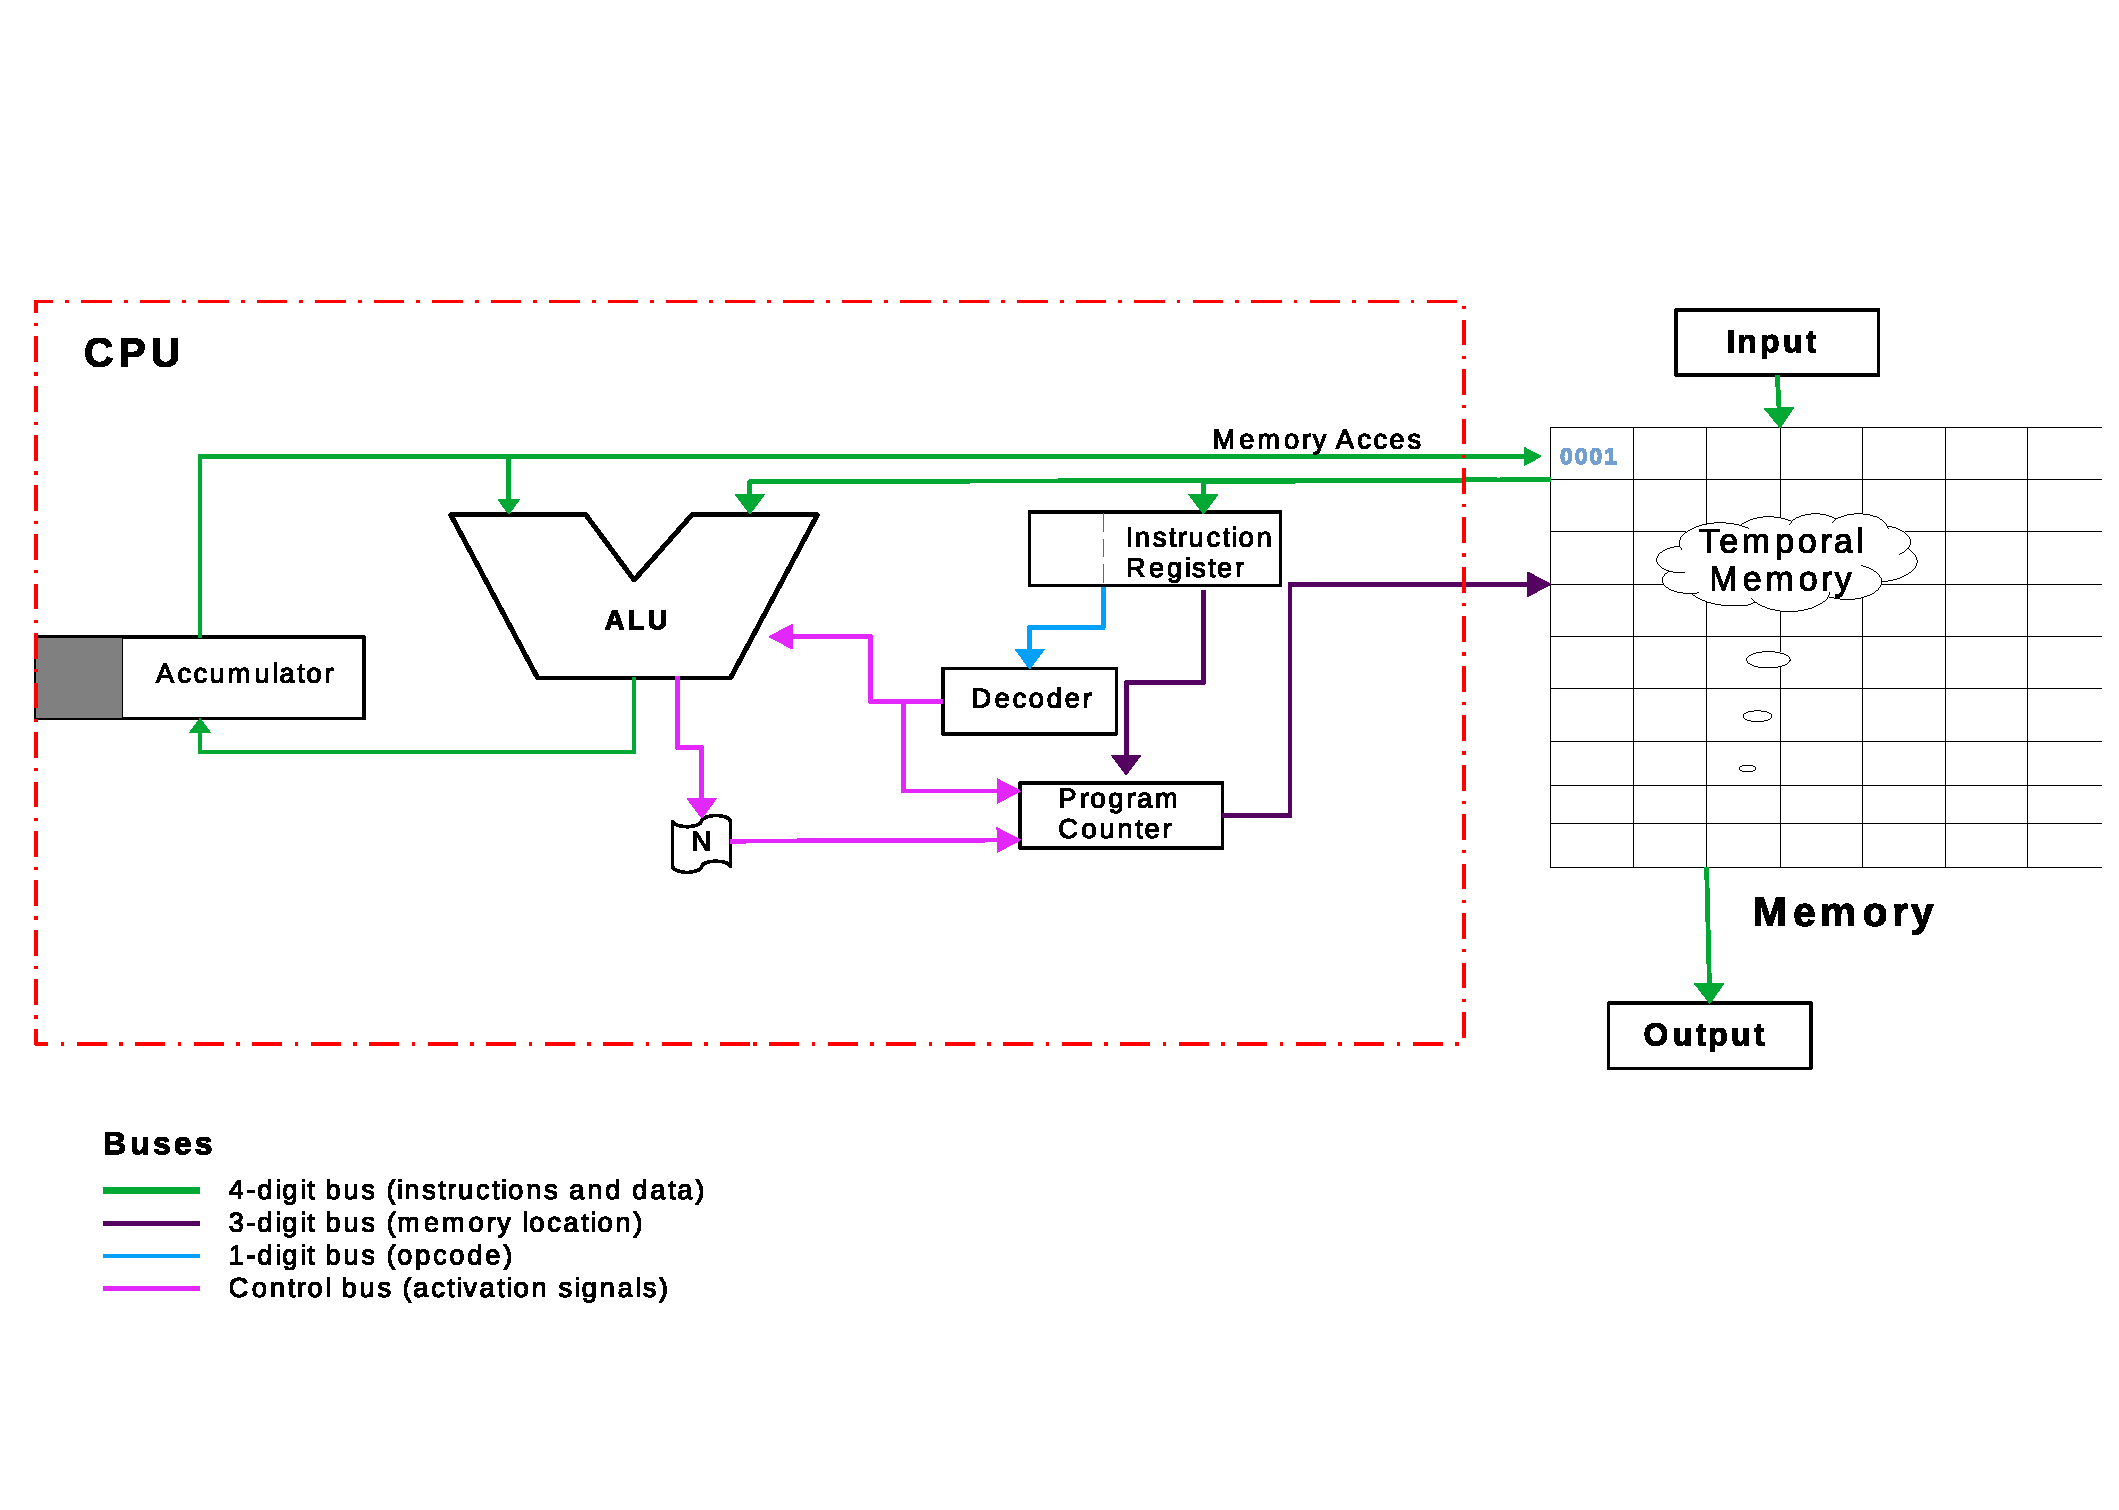
\includegraphics[scale=0.5]{media/CARDIACC/Arquitectura_diagrama_original.eps}
			\caption{Arquitectura de CARDIAC, concepto original Bell Labs \& Jorge Vasconcelos}
			\label{fig:Arquitectura_diagrama_original}
	\end{figure}
	
	
	
	El \textit{CPU} es la unidad dónde se concentran todos los elementos que hacen posible el cómputo de las instrucciones y datos
	que se almacenan en la memoria principal,
	está conformado por lo que está dentro de la línea punteada en rojo en la imagen \ref{fig:Arq_CARDIAC}, por la importancia
	de cada elemento dentro de la unidad de procesamiento central(\textit{Central Processing Unit}) se hará un repaso individual a cada uno.
	
	Revisemos cada elemento del CPU analizando sus funciones, para ello es preciso tener claro el concepto de \textbf{ciclo}, un
	ciclo completo es cuando regresas a la posición inicial, y algo parecido pasa con los ciclos en \textit{CARDIAC}. Un ciclo empieza
	cuando el \textit{Program Counter} o contador de programa apunta hacía una dirección, la primera sería la \#00, continua
	cuando la CPU toma el contenido de esa dirección y por medio del bus verde la transporta hacía el \textit{Instruction Register} o
	registro de instrucciones que se encarga de separar el dígito a extrema izquierda \textit{d2} para enviarlo al \textit{decoder}(decodificador)
	por medio de un bus azul y que esté decodifique que código de operación es para mandarle esa indicación a la \textit{Aritmetic Logic Unit (ALU)} o
	unidad aritmético lógica. Por otra parte, el mismo registro de instrucciones transfiere al contador de programa los dígitos \textit{d1} y \textit{d2}
	por si esté los ocupa para saltar a una dirección específica, si los ocupa el decodificador le enviará una señal por medio 
	del bus rosa para indicarle que los debe usar \cite{hegelbarger_instruction_1968}.
	
	Continuando con el \textit{ALU}, esté realiza la operación que le indica el código de operación, si el resultado que va a guardar
	en el acumulador es negativo manda una señal a \textit{Negative(N)} que es una especie de booleano, el cual indica si un número 
	que ha sido depositado en el \textit{Accumulator} o acumulador es
	o no negativo. Lo último que realiza el \textit{ALU} es almacenar el resultado de la operación en el  acumulador, un único registro
	que tiene la capacidad de almacenar sólo cuatro dígitos(uno más que la memoria principal), y es dónde se almacenarán todos
	los cómputos que realice el \textit{ALU} \cite{hegelbarger_instruction_1968}. 
	
	En caso de que la unidad aritmética requiera información
	de la memoria  para ejecutar una instrucción por medio de los buses verdes la puede recuperar directamente, dado que si requiere información
	de la memoria los dígitos \textit{d1} y \textit{d0} de la instrucción recogida por el registro tienen la dirección de dónde puede recuperarla, y es solamente
	si el \textit{ALU} obtiene el contenido de una dirección de esta forma que este será tratado como dato y no como instrucción. Si el contador de programa apunta a cualquier lugar de la memoria, el contenido de ese espacio será tratado como instrucción, a pesar
	de que no lo sea, lo que pude causar inconsistencias, por lo que hay que ser muy cuidadosos con lo que escribimos \cite{hegelbarger_instruction_1968}.
	
	De esta forma terminamos un ciclo cuando el contador de programa salta, que puede ser por qué una instrucción se lo indique, o bien porque
	el \textit{ALU} termino sus cómputos y entonces el contador de programa puede continuar a la siguiente dirección de forma incremental
	sin algún cambio \cite{hegelbarger_instruction_1968}.
	
	Los periféricos también juegan un papel importante, aunque solo se conectan directamente a la memoria principal, tanto el \textit{input} o entrada,
	como el \textit{output}(salida). Si se requiere imprimir algún resultado que esté en el acumulador, este debe ser enviado primero
	a la memoria principal para que se pueda realizar posteriormente la operación de impresión de un espacio de la memoria principal 
	\cite{hegelbarger_instruction_1968}.
	
	%%
	\subsection{Funcionamiento y lenguaje en CARDIAC}	
	
	Ahora conocemos los elementos de este modelo y como interactúan, pero lo visitamos de cierta forma ``a ciegas'', no conocemos el lenguaje
	que utiliza esta ``máquina'', y como mencionamos antes, tanto la máquina hace al lenguaje como el lenguaje a la máquina. En la tabla \ref{tab:simple-table} podemos ver el lenguaje que se usa en código, máquina(Código de operación) y 
	en 	ensamblador(Mnemotecnia) para CARDIAC que es mucho más fácil de entender, analizaremos cada una de las instrucciones presentadas
	originalmente en \cite{hegelbarger_instruction_1968} para entender la razón de su 
	existencia.
	
	
	\begin{table}[h]
	  \centering
	  \begin{tabular}{|c|c|p{8cm}|}
	    \hline
    	\textbf{Código de operación} & \textbf{Mnemotecnia} & \textbf{Definición} \\
	    \hline
	    0 & INP & (INPUT) Guardar tarjeta en memoria.\\
	    \hline
		1 & LDA & (LOAD)  Cargar en el acumulador información de la memoria.\\
		\hline
	    2 & ADD & (ADD)  Sumar al contenido del acumulador contenido en la memoria.\\
	    \hline
	    3 & BLZ & (Branch if Less than Zero) Saltar si la información en el acumulador es menor que cero.\\
	    \hline
	    4 & SHF & (SHIFT) Mover de izquierda y/o derecha el contenido del acumulador.\\
	    \hline
	    5 & OUT & (OUTPUT) Escribir en la salida el contenido de la memoria.\\
	    \hline
	    6 & STO & (STORE) Guardar información del acumulador en la memoria.\\
	    \hline
	    7 & SUB & (SUBSTRACT) Restar información de la memoria al acumulador.\\
	    \hline
	    8 & JMP & (JUMP) Saltar y guardar el valor del program counter en la dirección \#99. \\
	    \hline
	    9 & HLT & (HALT) Detener la ejecución del programa y reiniciar el contador del programa.\\
	    \hline
	  \end{tabular}
	  \caption{Lenguaje de programación de \textit{CARDIAC}.}
	  \label{tab:simple-table}
	\end{table}
	
	Para empezar necesitamos establecer una conexión entre el usuario y la máquina, que el usuario a través del dispositivo de entrada pueda
	darle información, con el código \textit{INP} podemos indicar el ingreso de información a la memoria principal, por ende con la instrucción  	
	\textit{012} estamos indicando que se guarde el dato que ingresa el usuario a través del dispositivo
	de entrada en la dirección de memoria 12, notaremos que en 9 de las 10 instrucciones los últimos dos dígitos hacen referencia a la dirección. 
	Posteriormente, necesitamos llevar información de la memoria al acumulador para realizar operaciones sobre ella, esto lo realizamos con el código 
	\textit{LDA}, por lo tanto, con la instrucción
	\textit{112} indicamos que se cargue en el acumulador la información almacenada en la dirección de memoria 12. Supongamos que el valor
	que ingresamos, y que fue guardado en 
	\#12 es \textit{005}, entonces \textit{005} será cargado en el acumulador. Ahora, si lo que queremos es incrementar el valor
	del acumulador en una unidad podemos usar el contenido de la dirección \#00, dónde se encuentra el dato \textit{001},
	mismo que podemos utilizar en la instrucción \textit{ADD} de la siguiente forma: \textit{200}, que indica que hay que sumar el contenido de la 
	dirección \#00 a lo que tiene
	el acumulador, obteniendo un \textit{006} en el acumulador.
	
	\begin{table}[h]
	  \centering
	  \begin{tabular}{|c|c|c|c|}
	    \hline
    	\textbf{Dirección \#} & \textbf{Código máquina} & \textbf{Ensamblador} & \textbf{Estatus acumulador} \\
	    \hline
	     20 & 012 & INP 12 & 000 \\
	     21 & 112 & LDA 12 & 005\\
	     22 & 200 & ADD 00 & 006\\
	     23 & 712 & SUB 12 & 001\\
	     24 & 712 & SUB 12 & -004\\
	     25 & 200 & ADD 00 & -003\\
	     26 & 325 & BLZ 25 & 000\\
	     27 & 200 & ADD 00 & 001\\
	     28 & 880 & JMP 80 & 001\\
	     29 & 212 & ADD 12 & 012\\
	     30 & 432 & SHF 21 & 020\\
	     31 & 613 & STO 13 & 020\\
	     32 & 513 & OUT 13 & 020\\
	     33 & 900 & HLT 00 & 020\\
	    \hline
	  \end{tabular}
	  \caption{Programa princiapl (In-Util). }
	  \label{tab:Programa_Principal}
	\end{table}
	
	Para seguir analizando los códigos de operación disponibles tenemos un código en la tabla \ref{tab:Programa_Principal} dónde
	podremos visualizar los códigos, su equivalente en ensamblador y como afectan al acumulador. Esté programa empieza en la
	dirección \#20, si nos damos cuenta las primeras tres instrucciones son las que revisamos en el párrafo anterior, y el
	estatus del acumulador expresa precisamente el valor que se mencionaba, el \textit{006}.

	Estamos ubicados en la dirección \#22, dónde nos moveremos a la \#23 en la que ocuparemos la instrucción de \textit{SUB} para restar, restaremos el 
	número que cargamos en la dirección \#12 a lo que tenemos en el acumulador, de hecho lo haremos dos veces seguidas para conseguir un número 	
	negativo, él \textit{-004}, si lo viésemos en operaciones matemáticas la operación sería la siguiente: $ 6-5-5 = -4 $. Los números negativos en este modelo son especiales, 
	como se habrá observado coloque el signo
	justo a la extrema izquierda, esto es porque para simplicidad del modelo los números negativos
	o positivos ocupan el mismo espacio, el signo siempre estará más a la izquierda que cualquier otro dígito, como las direcciones
	no pueden ser negativas no nos podemos encontrar con un caso del estilo \textit{1-42}, solo con casos como los del ejemplo, de modo
	parecido el modelo se toma la libertad de tomar al cero como positivo, situación que será importante con las siguientes instrucciones.
	
	Nos	movemos a la dirección \#25 en la que se suma un uno al acumulador y en la dirección \#26 ocupamos el código 
	\textit{BLZ} en la instrucción \textit{325} para obtener un salto condicional, es decir, si el contenido del acumulador es menor a cero salta a la 
	dirección \#25, por lo que se formara
	un bucle en el que el acumulador cambiara de valor de uno en uno hasta llegar a cero después de cuatro vueltas, momento en el que el condicional 
	dejara avanzar al contador de programa a la siguiente instrucción y no forzando el salto a \#25, pues, el valor del acumulador ya es
	positivo(para los fines del modelo).
	
	
	Lo que sigue es ver el funcionamiento de la operación \textit{JMP}, para esto continuamos con la ejecución, vemos que en la dirección
	\#27 se le suma un uno al acumulador para tener en el acumulador un \textit{001} y posteriormente ya está la operación
	de salto, que realiza uno a
	la dirección \#80, dónde se encuentra
	una \textbf{subrutina}, un programa ``pequeño'' generalmente usado por otros para reproducir un resultado. En este caso lo que hace
	es sumar un seis a lo que tenga el acumulador cuando el programa origen salte. Como nosotros tenemos un
	uno en el acumulador y queremos sumarle seis, la forma más fácil de hacerlo es saltando a esa subrutina que regresara a la dirección
	siguiente cuando termine, la \#29.
	
	Esté funcionamiento, lo podemos lograr fácilmente debido a que la instrucción \textit{JMP} al momento de saltar guarda la 
	dirección de memoria de la cual salta en la dirección \#99, con el sufijo \textit{8}. Si miramos la tabla \ref{tab:subrutina} dónde se encuentra
	está subrutina notaremos que lo primero que hace es cargar en el acumulador el contenido de la dirección \#99, que en
	esté caso es un \textit{828}, pues salto desde la dirección \#28, posterior se le suma un uno
	para así tener la dirección \#29, que es a la que tiene  que regresar la subrutina cuando termine, para lograrlo en la dirección
	\#82 indica que se guarde el resultado del acumulador en la última dirección de la subrutina, así cuando terminen todas las adiciones
	saltará a la dirección \#29.
	
	Como apunte importante, si leyeron el manual
	de \textit{CARDIAC} se habrán dado cuenta de que hay una ligera diferencia con la instrucción  \textit{Jump}, pues en el manual dice que guarda la dirección
	de la que salto más uno, es decir si salto de la dirección \#28 lo que se guardará en \#99 será la dirección \#29, un \textit{829}. Lo que en nuestro
	ejemplo particular ahorraría código, pero por los usos que se le dará en los siguientes modelos decidí que sería más eficiente como la he definido en esta sección, y esto
	es porque se tiene más precisión al tener la información más pura de dónde salto el programa. Y por supuesto, ambas definiciones pueden llegar a los
	mismos resultados con algunos cambios en la codificación.
	
	\begin{table}[h]
	  \centering
	  \begin{tabular}{|c|c|c|c|}
	    \hline
    	\textbf{Dirección \#} & \textbf{Código máquina} & \textbf{Ensamblador} & \textbf{Estatus acumulador} \\
	    \hline
	     80 & 199 & LDA 99 & 828 \\
	     81 & 200 & ADD 00 & 829 \\
	     82 & 690 & STO 90 & 829 \\
	     83 & 100 & LDA 00 & 001 \\
	     84 & 200 & ADD 00 & 002 \\
	     85 & 200 & ADD 00 & 003 \\
	     86 & 200 & ADD 00 & 004 \\
	     87 & 200 & ADD 00 & 005 \\
	     88 & 200 & ADD 00 & 006 \\
	     89 & 200 & ADD 00 & 007 \\
	     90 & 829 & JMP 29 & 007 \\
	    \hline
	  \end{tabular}
	  \caption{Subrutina para sumar varios unos.}
	  \label{tab:subrutina}
	\end{table}
	
	
	Continuando con el programa principal de la tabla \ref{tab:Programa_Principal} y habiendo regresado de la subrutina en
	la dirección \#29 con
	un valor en el acumulador de \textit{006} tenemos una suma que deja el valor del acumulador en \textit{012}, valor que será muy
	interesante para analizar el siguiente código de operación, \textit{shift/SHF}. Deje esté código para  casi el final 	
	por qué
	es la menos intuitiva, no es una de las operaciones básicas que usualmente tenemos en mente; sin embargo, cumple un papel fundamental, en las 
	computadoras binarias cumple un papel aún más crucial por las operaciones entre bits que se pueden realizar, pero en una decimal
	también aporta mucha flexibilidad y eficiencia en el uso de memoria para una gran variedad de operaciones.
	
	En la dirección \#30 vemos que el efecto de aplicar esta operación con la instrucción \textit{432} cambia el número \textit{012} por
	el \textit{20}. Esto sucede por qué el dígito \textit{d1} indica cuantos lugares a la izquierda se desplazará el valor
	del acumulador, dejando en 0 los espacios vacíos, mientras que el dígito \textit{d0} indica cuantos lugares a la derecha se desplazará.
	Aquí será muy importante la consideración especial de espacio que tiene el acumulador respecto a las celdas de la memoria principal, pues
	para evitar el desbordamiento accidental el acumulador siempre tendrá \textbf{un dígito más} del que las celdas de la memoria principal tengan,
	en este caso el acumulador puede almacenar hasta 4 dígitos.
	
	Si consideramos lo anterior y vemos la instrucción \textit{432} lo que nos indica primero es mover tres lugares a la izquierda
	el valor del acumulador, $0012$, dando como resultado $2000$, pues el \textit{1} queda fuera
	del espacio del acumulador, por lo que esté número se pierde para siempre y no se podrá recuperar. Si le aplicamos el desplazamiento de dos lugares 	
	a la derecha que se nos indica, terminaremos con $0020$ en el acumulador, como podemos ver el \textit{1} se perdió, y aunque desplacemos
	en el sentido contrario, si esté ya se quedó fuera del espacio del acumulador no podrá regresar. Para simplificar y como prácticamente no se usa el cuarto dígito dejamos indicado el resultado solo como $020$ en la tabla \ref{tab:Programa_Principal}.
	
	
	Para finalizar el programa tenemos en \#31 la instrucción para guardar la información del acumulador(\textit{STO}) en la dirección de memoria número
	\#13  y, posteriormente con el código  \textit{OUT} se establece la conexión con el dispositivo de salida para exportar los resultados
	que se guardaron en \#13, debido a que la instrucción \textit{513} indica con sus últimos dos dígitos la dirección
	de memoria de la cual se tomará la información. Finalmente, el programa se termina con el código  \textit{HLT}, marcando el
	final del programa y se reinicia el contador del programa
	a la dirección \#00, pues es lo que se indica con los dígitos \textit{d1} y \textit{d0} de la instrucción \textit{900}. Después de este repaso podemos constatar que en casi todos los códigos de operación los dígitos \textit{d1} y \textit{d0} hacen
	referencia a una dirección de memoria, salvo por \textit{SHF} en la cual tienen un funcionamiento especial.
	
	Con este lenguaje, simple, pero eficaz, podemos construir cualquier programa que queramos,
	puesto al tener ciclos, condicionales y la posibilidad de realizar
	las operaciones aritméticas básicas (suma y resta), podemos
	decir que es Turing completo, por lo que nuestra única limitante es la memoria.
	
	
	

	\clearpage	
	
\chapter{Evolución del Modelo}  %

	Como pudimos ver con anterioridad CARDIAC es sumamente útil para explicar aspectos importantes de la computación y el como se organizan sus 	
	componentes, sin embargo no podemos negar que a día de hoy es un tanto insuficiente para explicar las computadoras más modernas que tienen
	una concurrencia y un paralelismo sin los cuales no entenderíamos a las computadoras. No podemos imaginar una computadora en la cual no podamos 	
	ejecutar más de un proceso a la vez, por ello una evolución del modelo creado en los años 60 por \cite{hegelbarger_instruction_1968} es
	necesaria. Pero ello implica diferentes retos, retos que se abordarán en las siguientes secciones.
	
	Pero no solo en el apartado de diseño y organización del modelo se tendrá una actualización, sino también en la forma de presentarlo. Aprovechando
	las facilidades de algunos lenguajes de programación he realizado una simulación en Java para mostrar las mejoras realizadas al modelo
	original y que sea más sencillo mostrar la interacción de los distintos componentes de una computadora. La idea detrás de está simulación
	no es solo emular los comportamientos de CARDIAC en una computadora actual para ejecutar algunos programas,
	sino realmente realizar una \textbf{maquina virtual}, es decir un software que represente
	el modelo tanto a nivel Hardware como a nivel Software de manera virtual. En la imagen \ref{fig:welcomeec} tenemos la pantalla de inicio
	dónde se puede seleccionar la maquina virtual que queremos probar, como se podrá notar he agregado la iónica \textit{E}(de electrónico), que
	se puede apreciar en muchos productos a día de hoy, como sufijo de las tres maquinas virtuales para resaltar su aspecto
	electrónico distante del que tenía en los años 60. En la siguiente sección veremos algunos ejemplos de 
	programas
	de CARDIAC ejecutados en la maquina virtual \textit{E-CARDIAC}, para posteriormente adentrarnos en las evoluciones del modelo.

	
	\begin{figure}[h]
 			\centering
			\includegraphics[scale=0.5]{media/CARDIACC/WelcomeEC.png}
			\caption{Inicio para selección de maquinas virtuales}
			\label{fig:welcomeec}
	\end{figure}

	\clearpage
	\section{E-CARDIAC : Electronic CARDboard Illustrative Aid to Computation}
	
	Después de entrar al software de simulación y ver la pantalla de bienvenida como se ve en la figura \ref{fig:welcomeec} lo que sigue es elegir la maquina
	que queremos probar, en este caso comenzaremos con la versión que es prácticamente el modelo original
	llevado a un software de simulación. En términos
	generales las tres maquinas tendrán un esqueleto similar, por lo que una vez que conozcamos el funcionamiento de está primera será muy sencillo
	entender el funcionamiento de las otras dos aunque estás tengan más componentes. Para empezar será bueno visualizar el diagrama de la arquitectura de CARDIAC, diagrama 
	que se puede apreciar en la figura \ref{fig:arqCardiac} y que se irá comentando de acuerdo a los componentes a los que se haga referencia, pero
	como observación general se puede apreciar el CPU a la izquierda, la memoria a la derecha con una descripción de como son sus dígitos, y en la parte
	inferior las diferencias entre los buses que la componen así como el contenido de las celdas con información predefinida.
	
	\begin{figure}[h]
 			\centering
			\includegraphics[scale=0.5]{media/ECARDIAC/arq_cardiac.png}
			\caption{Arquitectura de CARDIAC por Jorge Vasconcelos, 2018}
			\label{fig:arqCardiac}
	\end{figure}	
	
	En la figura \ref{fig:iniECardiac} podemos ver el esqueleto de lo que será nuestra maquina que aún se encuentra apagada, por que al entrar
	lo que nos encontramos es una maquina apagada, que podemos encender al dar clic sobre el botón \textit{start}. Pero antes de dar clic ahí podemos
	ver que en esa barra principal tenemos varias opciones, a extrema izquierda está un símbolo de casa y un botón que dice \textit{CARDIAC Systems}, que
	nos permitirá regresar a la pagina de inicio si así lo deseamos. Continuando en el centro tenemos tres botones, el que ya vimos para encender
	la maquina, otro para pausar, algo poco común en una maquina de verdad, pero bastante usual en los software de maquinas virtuales, puesto
	que nos permite detener el funcionamiento completo sin afectar los procesos internos, analizar el estado
	de la maquina y después continuar como si nada hubiera pasado; el tercer botón es para reiniciar la maquina, un clásico en las computadoras.
	
	En la
	parte derecha de la misma imagen podemos ver dos casillas, una con un 100 y la otra con la palabra ``Normal'', estás son dos listas desplegables, la primera permite 
	elegir la cantidad de celdas con las que la maquina funcionara, es decir la memoria disponible, y la segunda es para elegir la velocidad de la maquina, de esa
	forma podemos decidir cuanto va a tardar cada ciclo en ser completado con el fin de observar el comportamiento de la maquina. En la figura \ref{fig:listasDespCardiac}
	podemos ver las listas desplegadas con las opciones que tienen disponibles, como podemos ver hay distintas velocidades para ver con más detalle el proceso
	en \textit{slow} o si queremos el resultado de inmediato está la opción \textit{instant}. En el caso de la memoria el funcionamiento es más interesante, pues
	no es solo una configuración externa a la maquina, sino que afecta directamente a la arquitectura y al lenguaje, puesto que con 1000 celdas el lenguaje
	debe cambiar para recibir direcciones de 3 dígitos, aunque el cambio en el lenguaje sería solo ese, por lo demás sólo sería la adaptación, mismo
	caso que para 10,000 celdas. Al elegir la cantidad de memoria y luego encender la maquina está se configura en su arquitectura para trabajar con esa
	cantidad de memoria y recibir instrucciones con direcciones más grandes.

	\begin{figure}[h]
 			\centering
			\includegraphics[scale=0.4]{media/ECARDIAC/ECARDIAC_P1.png}
			\caption{Pantalla de inicio de E-CARDIAC}
			\label{fig:iniECardiac}
	\end{figure}


	\begin{figure}[h]
 			\centering
			\includegraphics[scale=0.45]{media/ECARDIAC/ecardiac_lista_velocidad.png}
			\caption{Listas desplegables de E-CARDIAC}
			\label{fig:listasDespCardiac}
	\end{figure}

	

	Continuando con los elementos que tiene la maquina virtual podemos ver que en la parte izquierda de la figura \ref{fig:iniECardiac}  cuatro secciones, los
	componentes principales de la maquina en la
	\textit{Central Processing Unit}, el estado de la maquina en la parte del \textit{machinne status}, un apartado para las salidas en el \textit{output}, y un apartado en 
	blanco que servirá como cola de espera para la ejecución de las instrucciones\textit{queue}. En la primer sección, que es el \textit{CPU} podemos notar que está el
	registro de instrucciones(\textit{instruction register}) que contendrá la instrucción que viajo a través del bus verde desde la memoria al \textit{CPU}, después el 
	código de operación(\textit{Operational Code}) y el operando(\textit{Operand}) que son los resultados que presenta el decodificador(\textit{decoder} en la figura
	\ref{fig:arqCardiac}) después de que una instrucción pasa por el. Posterior se encuentra el contador de programa (\textit{Program Counter}),el componente que se 
	encarga de hacer avanzar la lectura de instrucciones sobre la memoria, el número que contenga el contador de programa es la dirección en la que se encuentra
	el ``puntero'' de la maquina, es decir que el contenido de tal dirección que es ``aputnada'' por el contador será transmitido al \textit{CPU}. Más abajo se
	encuentra el acumulador(\textit{Acumulator}) y la bandera para saber si un número es negativo(\textit{Negative}), el acumulador contendrá los resultados que arroje
	la unidad aritmético-lógica(\textit{ALU} en diagrama de CARDIAC) o bien algún valor que sea cargado directamente desde memoria por alguna instrucción como \textit{LDA}.                                                                                                                                                                                                                                                                                                                                                                                                                                                                                                                                                                                                          
	
	En la siguiente sección, \textit{Machinne Status} tenemos elementos externos a la arquitecrua de la computadora, y que más bien nos definen el
	estado de la maquina en cada momento, en cada ciclo que pasa nos indica directamente si la maquina está funcionando correctamente (\textit{CARDIAC is working}),
	pausada(\textit{CARDIAC is paused}) o si por el contrario dejo de funcionar(\textit{CARDIAC is dead}). Esté último puede ser causado por diversas razones
	que hagan que la maquina realice operaciones indebidas, como pasar un negativo como instrucción, para lo cuál la maquina no tiene respuesta
	y lo único que hará es detenerse. También en está sección está un apartado que indica la operación que estará ejecutando el \textit{CPU}.
	
	La tercera sección muestra la salida en forma de lista, como podemos ver en la figura \ref{fig:ecardiacOutput}, emulando lo que eran las salidas de las primeras 
	computadoras que podían imprimir resultados
	en cintas perforadas, permitiendo así al usuario ver el resultado de su programa; en está misma sección está un apartado para ``descargar'' la cinta y guardarla
	como un archivo de texto, que por defecto se guarda en la carpeta de descargas.

	\begin{figure}[h]
 			\centering
			\includegraphics[scale=0.27]{media/ECARDIAC/OutputFullfilled.png}
			\caption{E-CARDIAC Muestra de Output}
			\label{fig:ecardiacOutput}
	\end{figure}
	
	Toda la sección inferior está relacionada puesto que en la izquierda está la lista de instrucciones en cola por ser leídas(en \textit{Queue}),
	como en la figura \ref{fig:ecardiacQueue} se muestra, estás instrucciones
	el usuario podrá añadirlas  a la cola por parte del \textit{Deck Mode}, se podrán cargar desde ahí con solo escribirlas
	en forma de lista y dar clic en agregar tarjeta(\textit{Add Card}), como se ve en la figura \ref{fig:ecardiacDeckMode} dónde podemos ver una
	lista de instrucciones previo a ser añadidas a la cola. Por otra parte si se desea añadir instrucciones/datos de forma individual, uno a uno, se cuenta
	con la otra pestaña que dice \textit{Terminal Mode} y del cuál podemos ver un ejemplo de la carga en la figura \ref{fig:ecardiacTerminalMode}, pero para hacer uso
	de está pestaña es necesario que exista una instrucción que indique, como en el ejemplo, que dice que se espera una entrada en una celda, en caso contrario
	no se permitirá agregar datos de esa manera, puesto que esté modo transfiere directo los datos o instrucciones a la memoria en la posición solicitada,
	a diferencia del modo de tarjetas(\textit{Deck Mode}) que siempre primero las manda a la cola de espera, que las hará pasar posteriormente, cuando se solicite,
	a la memoria principal.


	\begin{figure}[h]
 			\centering
			\includegraphics[scale=0.4]{media/ECARDIAC/DeckModeLoaded.png}
			\caption{E-CARDIAC Carga masiva por tarjetas}
			\label{fig:ecardiacDeckMode}
	\end{figure}
	
	\begin{figure}[h]
 			\centering
			\includegraphics[scale=0.25]{media/ECARDIAC/TerminalMode.png}
			\caption{E-CARDIAC Carga individual de instrucciones}
			\label{fig:ecardiacTerminalMode}
	\end{figure}
	
	\begin{figure}[h]
 			\centering
			\includegraphics[scale=0.4]{media/ECARDIAC/QueueCargada.png}
			\caption{E-CARDIAC Lista de espera o cola de instrucciones/datos}
			\label{fig:ecardiacQueue}
	\end{figure}		
	

	Y ya en varias de las imágenes mencionadas en párrafos anteriores se mostró como se ve la memoria principal, pero vemos ahora la figura \ref{fig:enceCardiac} para
	ver la maquina cuando acaba de encender y centrémonos en la memoria principal, compuesta de 100 celdas numeradas del 00 al 99 con los datos
	por defecto que tienen en esas especies de memorias ROM. En color blanco con fondo gris están todas las direcciones de memoria, y con un fondo blanco pero
	contenido en negro los datos que contiene cada dirección, y para diferenciar la dirección de la celda de la cuál el contenido está siendo transmitido
	al \textit{CPU} de la maquina se tiene el color azul marino, en el caso del ejemplo nos indica que se está leyendo la instrucción en la dirección \#00.
	
	%
	
%
	
	\begin{figure}[t!]
			\includegraphics[scale=0.28]{media/ECARDIAC/ECARDIAC_P2.png}
			\caption{E-CARDIAC después de iniciar sus funciones}
			\label{fig:enceCardiac}
			
	\end{figure}
	
	
	De esta forma terminamos el recorrido por la maquina virtual de \textbf{E-CARDIAC} que nos permitirá experimentar con más soltura la programación en
	lenguaje ensamblador, el lenguaje ensamblador particular de está maquina, además de que tenemos la posibilidad de hacer crecer su memoria principal aumentando
	así las posibilidades que nos da está maquina. Y precisamente la siguiente evolución del modelo requerirá de un aumento en la memoria de CARDIAC que es muy fácil
	de aplicar sobre la maquina virtual puesto que desde el principio se considero esa posibilidad, y que podremos estudiar con más profundidad en la siguiente
	sección.


	\clearpage	
		
	\section{E-CARDIAC C : Electronic CARDboard Illustrative Aid to Concurrent Computing}
		
	El nombre es un homenaje al lenguaje de programación \textbf{C}, agregando esa ``C'' al final del nombre que tenía el modelo anterior
	para expresar que la diferencia entre estos dos es la concurrencia. \textit{E-CARIDAC C}, ayuda ilustrativa de cartón electrónico para
	la computación concurrente, por sus siglas en inglés, tiene la intención de ser un modelo que represente la organización de una computadora que puede tener operaciones concurrentes
	y poder ver como interactúan las distintas partes de la computadora para lograr la concurrencia. Buscamos la concurrencia a nivel procesos
	en este caso, dado que generalmente es utilizada en las computadoras comunes. Esto nos lleva a tener que hacer varios cambios en el diseño original
	del modelo, agregar mecanismos en el Hardware, en el Software y diseñar una especie de sistema operativo para poder lograr la concurrencia de 
	procesos.
	

	
	
		\subsection{Necesidad de un sistema operativo}
		
		El primer paso es entender la necesidad de tener un sistema que administre los recursos de la maquina, sin ello podemos construir muchos programas, pero
		la ejecución deberá ser individual a nuestra disposición, de cierta manera seríamos nosotros mismos ese sistema de administración. Si bien en 
		\cite[p. 42]{hegelbarger_instruction_1968}
		nos presentan un sistema de carga de programas para el modelo original, un bootloader diseñado para poder escribir en ``tarjetas'' un programa y que se vaya
		añadiendo a la memoria de CARDIAC sin la necesidad de literalmente colocar en los espacios de memoria de CARDIAC las instrucciones, esto aún nos deja
		con la tarea de decidir que programa va primero. Así que partiendo de este punto podemos concluir que el programa que realice esa tarea será un sistema
		operativo mínimo, y necesita el sufijo de mínimo por que la otra característica que define
		a un sistema operativo es ser una capa de abstracción entre la maquina y otros programas, como puede ser un teclado o un sistema de audio que estén programados
		para funcionar sobre un sistema operativo y no directamente sobre la maquina, por ende la maquina podría cambiar y el programa seguir funcionando. En este
		caso este sistema operativo que se diseñará no tiene la intención de ser una capa de abstracción tan marcada, tendrá algunos aspectos que pueden ser considerados
		un capa de abstracción entre los programas y la maquina, pero no lo será completamente. Por tal razón lo nombraremos como sistema operativo mínimo o SOM
		en el resto del texto.
		
		Entendiendo un programa que realice tal tarea parece evidente que el espacio de memoria del modelo original será insuficiente, por lo que una de las necesidades
		derivadas del SOM será la ampliación de la memoria, lo que llevará a un cambio también en el lenguaje que esa diseñado específicamente para direcciones de dos 
		dígitos. Y seguramente la implementación de un sistema operativo requerirá de algún sistema de almacenamiento secundario para el programa, de forma que no esté
		cargado directamente en la memoria principal como si de una memoria ROM se tratará, esto derivaría en la necesidad de conectar ese almacenamiento secundario
		con la memoria principal y por ende aumentar la cantidad de buses. Además al ser un programa que requiera unos privilegios de control de la maquina más elevados
		quizá se necesiten piezas de hardware que en su versión original CARDIAC no necesitaba.
		
		\subsection{Mejoras necesarias en el Hardware}
		
		Para solucionar las necesidades mencionadas más arriba decidí aumentar las celdas de memoria de 100 a 1000, de forma que cada dirección posible tendrá
		tres dígitos, de forma que un número completo de cuatro dígitos	puede representar tanto el número en si mismo, como un código de operación acompañado de una
		dirección. Por ende los buses deberán ser capaces de transmitir más dígitos que en el modelo original, en la figura \ref{fig:diagarquiConc} 
		podemos observar
		en la parte inferior izquierda como serán los buses; los de color verde, que son los de mayor capacidad, transmitirán instrucciones y datos, los
		que están en color morado sólo las direcciones, mientras que los que están en color azul sólo los códigos de operación. Adicionalmente hay unos buses
		en color rosa que transmitirán señales de activación. En la misma imagen se puede apreciar que al principio y al final de la memoria las celdas no han cambiado
		mucho, al principio está un valor que será inmutable que tiene el mismo significado que en el modelo original salvo que con un cero extra por el crecimiento
		en el tamaño de la memoria, y la misma situación la tiene el valor del final de la memoria, que solo podrá contener un valor el cuál inicie con un $8$, y
		que por defecto será $8000$, el sufijo que sigue al código de operación $8$ será la dirección de memoria de dónde se tomo una instrucción de salto 
		que fue ejecutada.
				
		\begin{figure}[h]		
			\centering
			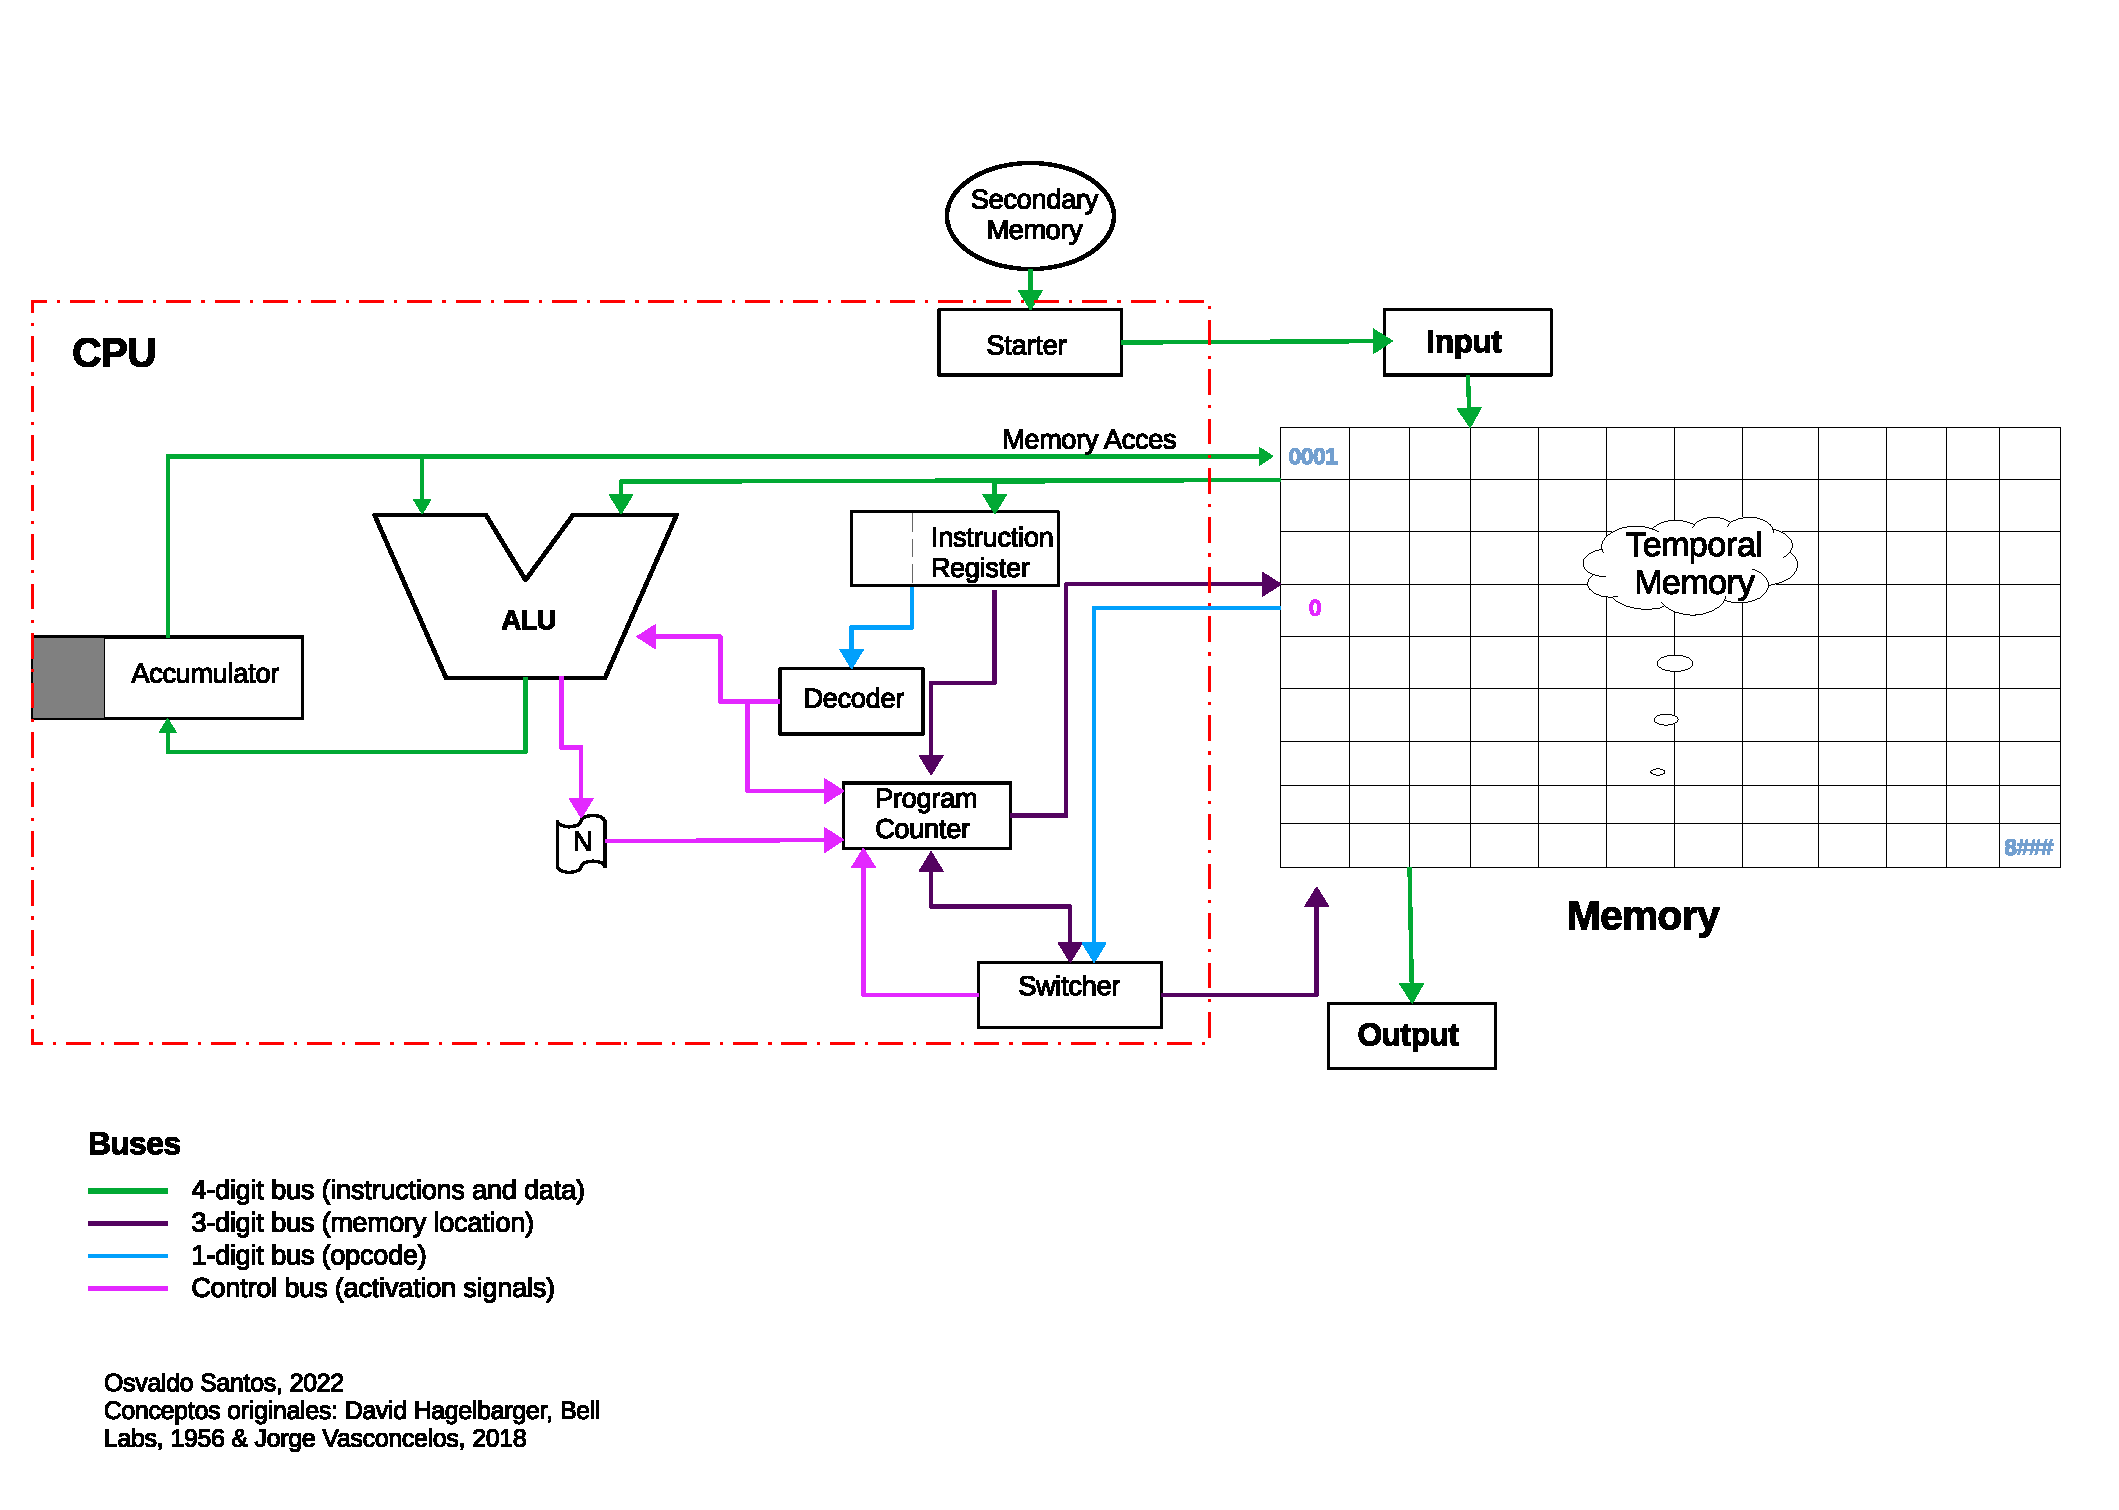
\includegraphics[scale=0.5]{media/CARDIACC/Arquitectura_diagrama_concurrente.eps}
			\caption{Diagrama de Arquitectura de E-CARDIAC C}
			\label{fig:diagarquiConc}
		\end{figure}
		
		
		Esto permite mantener varios elementos del funcionamiento del modelo original sin cambios, pero podemos notar tres de elementos nuevos, que a su vez
		incrementan el número de buses presentes en el modelo. Detengámonos primero en el que está conectado al \textit{input} en la parte superior del centro,
		el que tiene por nombre \textbf{starter}(iniciador) y que a su vez está conectado con otro elemento nuevo llamado \textbf{secondary memory}(memoria secundaria).
		La memoria secundaria es la representación de lo que vendría siendo el disco duro en las computadoras, pero más limitada por que sólo sería de un almacenamiento
		muy puntual para el sistema operativo, que tendría que hacerse por fuera de la computadora, y siendo más bien como una tarjeta con un programa especifico que
		está conectada a través del \textbf{starter} para que apenas se inicie la maquina lo primero que haga es empezar a agregar las instrucciones guardadas
		en la memoria secundaria a la pila de ejecución que recibe el \textit{input}. De está manera podemos mantener simple el modelo, pero establecer una conexión
		con otra fuente de información diferente a la memoria principal, y poder colocar el sistema operativo mínimo de una forma más natural sin que esté ahí
		desde siempre como si fuera parte de la memoria ROM.
		
		
		El otro integrante de este nuevo modelo es el que tiene por nombre \textbf{switcher}(cambiador) que está en la parte inferior derecha del área del CPU,
		esté elemento es la solución al problema que tiene la inclusión de un programa que necesita tener los privilegios de poder tomar el control de las ejecuciones,
		cederlo a otros programas, pero también recuperarlo en un momento particular. Como se puede observar en la imagen tiene 4 diferentes conexiones, siendo uno
		de los que más tiene, y su función radica en que cada \textbf{N} ciclos dar manda una señal(con el bus rosa) al contador de programa para que salte a la dirección 
		de inicio del sistema operativo, dirección que tiene que ser establecida en la configuración de la misma maquina. Esto lo hace siempre y cuando en la dirección
		\#003 el valor que esté ahí sea $1$, que indica que es tiempo de ejecución del usuario y por tanto cada N ciclos los recursos regresan al SOM, si
		el valor fuese un $0$, como es por defecto, no haría esos saltos, puesto que significa que los recursos los tiene el SOM, el cuál puede disponer
		de ellos sin limite al tener todos los privilegios posibles. Está conexión se hace con un bus que azul pues solo requiere de un dígito, además contiene
		una conexión bidireccional al contador de programa que le permite contar los ciclos que han sucedido e indicarle al contador de programa a que dirección
		tiene que saltar cuando se trata de regresar el control de los recursos al SOM, aquí se requiere un bus de color morado puesto que requiere de una
		capacidad de 3 dígitos. La otra razón de está conexión bidireccional es que el \textbf{switcher} recibe del contador programa la última dirección
		apuntada por el proceso del usuario, antes de que fuera ejecutada puesto que para ese momento si se llegaron a los N ciclos se da la instrucción
		de regresar los recursos al SOM y al mismo tiempo la instrucción es transmitida al \textbf{switcher} para que este por medio de su conexión a la memoria principal
		la coloque en una dirección especial de la cual el SOM podrá recuperarla para después cuando regrese los recursos a es proceso pueda continuar
		justo en el punto que había dejado.
		
		El sistema operativo mínimo en su mismo proceso ejecuta otros procesos y por ende realiza los saltos necesarios para ceder los recursos, pero antes de ejecutarlos		
		modifica el valor de la dirección $\#003$ a $1$ para que el \textit{switcher} pueda regresar el control al SOM después de N ciclos aproximadamente,
		para lograr la consistencia en la ejecución de procesos en el momento que la bandera es cambiada el contador del \textit{switcher} se reinicia. Aclarando
		la parte de ``N ciclos aproximadamente'' es por que
		una vez que es cambiado el valor a a $1$ por el SOM en la dirección que funge como \textbf{bandera de saltos} aún ejecutará un par de instrucciones propias
		del SOM para lanzar otros procesos, por lo que en realidad el proceso del usuario tendrá $N-2$ ciclos disponibles.
		
		Por supuesto con todos estos cambios hechos para poder instalar un sistema que administre la ejecución de procesos concurrentemente el lenguaje también
		requiere modificaciones, en su mayoría mínimas, pero otras que van orientadas totalmente a funcionar con un sistema operativo.
		
		\subsection{Cambios en el lenguaje}
		
		Como ya leímos en secciones pasadas el lenguaje de una maquina muchas veces es consecuencia de las posibilidades que el hardware proveé a la maquina, pero
		también el lenguaje define ciertas necesidades del hardware, por lo que en la construcción de una maquina se necesita pensar en todos
		los elementos que van a interactuar juntos. Para este caso agregamos un nivel extra, la consideración del sistema operativo mínimo, pues como
		podemos notar en la tabla \ref{tab:programing_language_ecc} uno de los únicos dos cambios que hubo es en la instrucción \textit{halt}, está
		esta diseñada ahora para funcionar con un sistema operativo, pues por si sola no tendrá las capacidades completas que si tendrá con un SOM. En la
		configuración inicial de la maquina se definirá la dirección que está definida como ``área de borrado'' para el SOM, y es con este detalle
		que podemos considerar que nuestro SOM es en cierto punto una capa de abstracción entre el código maquina puro y lo que harán los procesos,
		que será comunicarse con el SOM y el se comunicara con la maquina, en este caso para detener el proceso.

		
		
			\begin{table}[h]
			  \centering
			  \begin{tabular}{|c|c|p{8cm}|}
			    \hline
		    	\textbf{Código de operación} & \textbf{Mnemotecnia} & \textbf{Definición} \\
			    \hline
			    0 & INP & Guardar tarjeta en memoria.\\
			    \hline
				1 & LDA & Cargar en el acumulador información de la memoria.\\
				\hline
			    2 & ADD & Sumar al contenido del acumulador contenido en la memoria.\\
			    \hline
			    3 & BLZ & Saltar si la información en el acumulador es menor que cero.\\
			    \hline
			    4 & SHF & Mover d2 veces a la izquierda el número y d1 veces a la derecha el número.\\
			    \hline
			    5 & OUT & Escribir en la salida el contenido de la memoria.\\
			    \hline
			    6 & STO & Guardar información del acumulador en la memoria.\\
			    \hline
			    7 & SUB & Restar información de la memoria al acumulador.\\
			    \hline
			    8 & JMP & Saltar y guardar el valor del program counter en la dirección \#999. \\
			    \hline
			    9 & HLT & Detener la ejecución del programa y saltar al área de borrado de procesos del SO, no importa el valor que los dígitos d0,d1, y d2 tengan\\
			    \hline
			  \end{tabular}
			  \caption{Lenguaje de programación de \textit{E-CARDIAC C}.}
			  \label{tab:programing_language_ecc}
			\end{table}

		El otro cambio a destacar es en la instrucción \textit{shift}, considerando el dígito a extrema izquierda como \textit{d3} y el resto de manera descendente
		hasta llegar a \textit{d0} a extrema derecha, tenemos que el dígito \textit{d3} tendrá el \textit{opcode} como en todas las demás instrucciones. Pero
		para está solo importarán los dígitos \textit{d1} y \textit{d0}, puesto que el \textit{d2} no representará nada en la instrucción, de está forma
		se mantiene el funcionamiento del modelo original de mover el número de izquierda a derecha una cantidad determinada de veces.
		
		El último cambio a destacar es que el valor del \textit{program counter} que se guardaba en \#99 cuando se hacía un salto con la instrucción \textit{jump} ahora
		será guardado en la dirección \#999, que es la última en está arquitectura. Pero para todas las instrucción, a excepción de \textit{halt} y \textit{jump},
		el comportamiento será el mismo sólo que los tres dígitos de la derecha representan la dirección, lo cuál es bastante lógico dado que las direcciones
		ya no ocupan dos dígitos, sino tres.
		
		Con esto tenemos el diseño completo de la maquina, su arquitectura, y su lenguaje. Ahora podemos dar el paso a escribir el sistema operativo mínimo que
		pueda realizar las tareas que esperamos en está maquina, aunque por supuesto y como se dijo ya se había pensado en que características necesitaba la maquina
		para poder implementar un SOM y que tipo necesitaría.

		
		\subsection{Sistema Operativo Mínimo C}
		
		Conocemos ahora los aspectos esenciales que debe tener un proceso para ser un sistema operativo y las necesidades particulares que tiene
		el que necesitamos implementar en nuestro modelo, por ende detrás de el desarrollo de esté sistema operativo
		mínimo, llamado \textit{SOMC}, está una lista de tareas que debe ser capaz de realizar para poder ejecutar concurrentemente diferentes procesos,
		en las siguientes secciones iremos viendo cada una de esas tareas.
		
		El diseño de este programa lo hice pensando en una arquitectura de mil celdas, pero que pudiese ser extensible a más, para ello era necesario
		que las direcciones no fuesen fijas en el diseño del programa, por lo que use variables para las direcciones, de forma que en
		el diseño puedo tener una dirección como \#s1, pero en la implementación esa dirección se transforma en \#801, así si tenía una
		instrucción de la forma \textit{1(s1)} su transformación será \textit{1801}. De está manera tenemos mucha flexibilidad al momento de escribir
		el código del programa, cuando comencé pensé que con menos de 100 celdas de memoria podría escribir todo el programa, por ende que iniciara
		en la celda \#900 parecía razonable, pero a medida que avance
		descubrí que no, y está flexibilidad en cuanto a las direcciones me permitió seguir escribiendo para más de 100 direcciones sin tener que reescribir
		lo que ya tenía, lo único que tenía que hacer es cambiar la dirección de inicio de mi programa, si antes \#s0 erá \#900 ahora sería \#800 y lo mismo
		pasaría para sus consecutivos.
		
		Otra parte importante para mantener está flexibilidad fue dividir el programa en diversos segmentos, el principal es el núcleo del
		sistema operativo mínimo y que lleva tal cuál ese nombre, otro es la \textbf{zona de procesos} para almacenar el contexto de los
		procesos que se estén ejecutando en la maquina, y además por separado está una \textbf{zona de variables} que serán variables o constantes de uso recurrente
		que el sistema operativo mínimo pueda guardar o consultar, y por último un segmento llamado \textbf{preámbulo} que serían las primeras instrucciones
		que se ejecutan cuando el SOM toma control de los recursos y prepara así ciertas variables para que cuando el núcleo del SOM esté en ejecución
		todas las variables estén en su correcta posición. Las ventajas de segmentar el programa es que puedo cambiar las direcciones de inicio de cada segmento
		una vez que ya tenga todo escrito sin afectar la estructura del código.

		
		Adicionalmente en el núcleo del SOM también agregué una especie de segmentación en cuanto a las tareas que realiza cada sección del SOM, separandolas en:
		añadir proceso, actualizar proceso, borrar proceso, ejecutar proceso, y ejecución de bootloader. Para poder seguir todos estos conceptos con más claridad
		también diseñe un diagrama de flujo, que se puede ver en la imagen \ref{fig:diagramaSOMC}
		, en el cuál cada sección está con un color diferente. Por el tamaño del diagrama es dificíl apreciar los que dicen las letras, pero
		en cada sección que ocupemos de una parte del diagrama se le hará un acercamiento a esa zona, pero para darse una idea
		de las conexiones entre cada zona está imagen es de mucha ayuda.
		

		\begin{figure}[p]		
			\centering
			
\includegraphics[width=\textwidth,height=\textheight,keepaspectratio]{media/CARDIACC/Diagrama_Flujo_SO.eps}
			\caption{Diagrama de flujo de SOMC}
			\label{fig:diagramaSOMC}
		\end{figure}		
		

		
		\subsubsection{Nomenclatura del diseño del código}
		
		Para explicar el código del sistema utilizaré además del ya mencionado diagrama imágenes como la de la figura \ref{fig:somcPreambulo}, dónde
		se puede ver el código, así como una descripción de cada instrucción. A la izquierda está el ``nombre clave'' de cada dirección o grupo
		de direcciones si es que lo necesitan, es una descripción corta acerca de esas direcciones, por ejemplo en las instrucciones
		coloreadas de color rosa hay un nombre clave que indica que es una bandera; en la parte del medio tenemos la dirección de memoria, después
		la instrucción en lenguaje maquina, y al lado la instrucción en lenguaje ensamblador, para finalizar en la parte derecha con la descripción completa
		de la instrucción si está fuera necesaria. Cada sección del SOM tendrá variables de direcciones diferentes, así
		para el preámbulo las variables que indiquen las direcciones empezaran por una \textit{e} y continuarán de forma serial. En las columnas
		dónde están las instrucciones podemos ver como se usaran, si nos fijamos en la fila dónde está la dirección \#e10 veremos la instrucción
		\textit{1(e(0)}, que indica que se cargue el contenido de la dirección \#e0 en el acumulador, en la implementación la variable
		de dirección sería sustituida por una dirección real de la maquina.
		
		Así como para el preámbulo las variables de direcciones empiezan por \textit{e}, para la zona de procesos empezaran por \textit{p},
		en la zona de variables del sistema por \textit{c} y las del núcleo del sistema operativo empezarán por \textit{s}. De está forma
		también será rápido en el código identificar a que zona está haciendo referencia la instrucción, por ejemplo en la imagen
		del preámbulo en la fila de la dirección \#e6 se encuentra una instrucción de la forma \textit{2(c13)}, lo que ya nos indica
		que va a trabajar con un valor de la zona de variables del sistema por la letra \textit{c} que se encuentra en el interior
		de la instrucción, examinándola nos dice que se va sumar al contenido del acumulador el contenido de la dirección \#c13, y tanto
		la descripción como el nombre clave nos proveerán de el contexto de la instrucción para entender su significado.
		
		\begin{figure}[h]		
			\centering
			\includegraphics[scale=0.45]{media/CARDIACC/Preambulo.png}
			\caption{SOMC:Preámbulo}
			\label{fig:somcPreambulo}
		\end{figure}
		
		\subsubsection{Inicio de operaciones para la maquina}
		%%Investigar lo que se dijo del bootloader antes
		
		El sistema operativo mínimo estará en la memoria secundaria y para poder proceder con su carga automática y que para el usuario sea transparente se
		requiere de un sistema de arranque o sistema de \textit{booteo}, para esto las instrucciones que el \textit{starter} mande a la cola y se empiecen a ejecutar
		para cargar el sistema en la memoria principal deben estar en forma de tarjeta, es decir una instrucción o dato seguida de otra en forma de lista,
		deben empezar siempre por las siguientes:

		\begin{center}
		\begin{minipage}{0\textwidth}
			\begin{verbatim}
				0002
				0008
			\end{verbatim}	
		\end{minipage}
		\end{center}
		
		con estas instrucciones de inicio basta para que las siguientes sólo tengan que ser pares de instrucciones dónde la primera indica el destino de la segunda
		para que se pueda cargar por si misma el resto de la tarjeta, abajo vemos cuales serían 
		las siguientes instrucciones a ejecutar:
		
		\begin{center}
		\begin{minipage}{0\textwidth}
			\begin{verbatim}
			0003
			0000
			0004
			0000
			\end{verbatim}	
		\end{minipage}
		\end{center}
		
		Son pares de instrucciones, el primer par es para cargar la bandera que indica si es un proceso del usuario o uno del SOM el que está en ejecución,
		como notamos la primer instrucción del par indica que la segunda sea cargada en la dirección \#003 y que el valor cargado ahí es un 0000, puesto
		ahí por defecto para indicar que los recursos son del SOM. El siguiente par lo que nos indicará es el identificador o ID del proceso
		que se está ejecutando en ese mismo momento, y no se escogido el 0 sólo por ser un número por defecto, es por que justamente se está ejecutando el 
		\textbf{proceso 0}, puesto que para el SOM este sistema de \textit{booteo}, una vez que ha arrancado la maquina, al ejecutar las primeras dos instrucciones
		se transforma en un proceso que es parte del sistema operativo y que será gestionado como tal, pero con algunas características especiales que son
		causantes a su vez que se tenga un color especial en el diagrama y en el código cuando el SOM tiene que hacer operaciones referentes al proceso 0.
		
		%% Anexo 2
		Lo siguiente que vendrá en la tarjeta es todo el contenido de cada segmento del sistema operativo, la tarjeta usada para cargar el sistema
		se encuentra completa en el anexo 2 para su consulta, pero básicamente son pares de instrucciones que para colocar cada segmento
		del sistema en su lugar.
		
		\subsubsection{Encendiendo la maquina}
		
		En la figura \ref{fig:eccApagada} podemos observar  como será la maquina virtual para esté modelo y nos ayudará como guiá para comprender muchos
		de los aspectos del modelo. Podemos ver que ahora en la parte inferior derecha ya no hay un espacio vacío como en la primer maquina, sino que se encuentra
		el contenido de la memoria secundaria(\textit{Secondary Memory}), que tiene una dirección de memoria(en la secundaria) y el contenido, si oprimimos \textit{Start}
		el contenido de la memoria secundaria se mueve a la cola de ejecución(\textit{Queue}), pero no desaparece de la memoria secundaria como podemos
		ver en la figura \ref{fig:eccEncendida1}, sino que al ser está una memoria no volátil o 
		permanente se queda ahí estática, no cuenta como memoria ROM por que es posible
		reescribirla, pero de forma externa, lo podemos pensar como que es una tarjeta que se puede cargar, una cinta que se le puede colocar a la maquina para que
		está a través del \textit{Starter} la coloque en la cola. Como se notará en las imágenes otra parte que cambio fue la parte del estatus de
		la maquina, que ahora tiene un campo llamado \textit{Starter} que en la maquina apagada tiene un valor de ``Waiting'' y en la encendida de ``Booted'', esto
		es por que al encender el starter en automático ha colocado la tarjeta de la memoria secundaria en la cola, solo es cuestión de dejar seguir la ejecución
		para que la carga se complete.

		\begin{figure}[h]		
			\centering
			\includegraphics[scale=0.25]{media/CARDIACC/ECARDIACC_apagada.png}
			\caption{E-CARDIAC C Apagada}
			\label{fig:eccApagada}
		\end{figure}		
		
		\begin{figure}[h]		
			\centering
			\includegraphics[scale=0.25]{media/CARDIACC/ECARDIACC_encendida1.png}
			\caption{E-CARDIAC C durante el arranque}
			\label{fig:eccEncendida1}
		\end{figure}
	
		Aparte del \textit{Starter} tenemos otros tres campos que nos ayudaran a ver quien tiene el control de los recursos y por cuantos ciclos, el campo
		\textit{Limit of Cycles} contiene el valor de cuantos ciclos máximos tendrá un proceso del usuario antes que obligadamente tenga que ceder
		los recurso de nuevo al SOM, la implementación que se muestra tiene un máximo de 30 ciclos para cada proceso del usuario. El \textit{Counter SW} tiene
		un contador de ciclos pero a diferencia de \textit{Cycle} esté se reinicia cada que el control de los recursos cambia de propietario, si está
		ejecutándose un proceso del usuario cuando esté contador alcance el mismo número que tiene \textit{Limit of Cycles} el \textit{Switcher} saltará
		de inmediato al preámbulo del SOM para que esté tome control de los recursos, si es al revés el contador sólo nos servirá de indicador
		de cuantos ciclos lleva el SOM desde que le cedieron los recursos, pero como la bandera se encuentra en 0 si el control lo tiene el SOM el switcher
		no podrá hacer ningún salto. Para saber quien tiene el control también podemos ver el último campo, el \textit{SW Status} que nos indicará quien tiene
		el control de los recursos, en las imágenes lo tiene el SOM y por eso tiene un valor de \textit{SO} si fuera un proceso del usuario tendría \textit{User}. Es
		importante mencionar que las primeras instrucciones del preámbulo son consideradas aún como parte del proceso del usuario para el estatus por que
		en esas primeras instrucciones se cambia la bandera de valor, aunque para el contador del \textit{switcher} esto ya se contempla como parte del
		proceso del SOM.
		
		Lo que sucede una vez que el sistema ha sido cargado en la memoria lo podemos ver en la figura \ref{fig:eccSOMcargado}, dónde podemos ver que el
		puntero está en la dirección \#000, es decir está esperando un dato para cargarlo en la dirección \#001, que ya tiene un dato que fue cargado
		en algún momento durante la carga del SOM en memoria. También podemos ver que las banderas están cargadas correctamente y algo que nos puede llamar la atención
		es que el \textit{SW Status} marca que el control de los recursos lo tiene el sistema operativo, y esto no es un error, por que parte de los permisos especiales
		que tiene el proceso 0 es que no tiene un límite para ceder los recursos, es una extensión del mismo sistema operativo, por que es el proceso que va a permitir
		al usuario cargar programas para que sean ejecutados, y no sería nada optimo que cada N ciclos tuvieras que detener la carga de programa para que otro se ejecute,
		la carga de programas por el usuario tiene el privilegio más alto entre los procesos, y sólo el usuario cuando haya cargado los procesos
		que quiera cederá el control al SOM para que administre los recursos y empiece la ejecución de los procesos previamente cargados.
		
		\begin{figure}[h]		
			\centering
			\includegraphics[scale=0.25]{media/CARDIACC/ECARDIACC_socargado.png}
			\caption{E-CARDIAC C Sistema operativo mínimo cargado}
			\label{fig:eccSOMcargado}
		\end{figure}
		
		
		\subsubsection{¿Como toma control el sistema operativo mínimo?}
		
		Como pudimos ver en las imágenes anteriores, a pesar de que para el \textit{switcher} el control de los recursos este actualmente del lado
		del SOM, la realidad es que no controla los recursos y más bien es el usuario, aunque no unos de los procesos del usuario, quien controla
		los recursos. En la figura \ref{fig:diagramaSOMC} que nos presenta un diagrama de flujo muy general podemos alcanzara ver tres recuadros
		rosas que tienen una forma más inclinada que la de un rectángulo normal, esto es por que serían entradas de datos por parte del usuario, y
		que en el diagrama use para ejemplificar las tres formas en que el SOM toma de nuevo el control de los recursos; la primera es cuando
		el va a añadir un nuevo proceso, la segunda cuando el contador de programa por medio del \textit{switcher} salta en automático, y la tercera
		si se da la indicación de borrado de un proceso, es decir si se lee la instrucción \#9000.
		
		
		En la figura \ref{fig:eccSOMCdiagent} apreciamos estás tres formas en que el sistema entra en acción como tal, y podemos notar que todas van a instrucciones
		de color café siempre, esto es por que siempre antes de llegar al núcleo del SOMC se debe pasar por el preámbulo que se encarga de actividades previas
		a las ya mencionadas para que estás puedan llevarse a cabo con normalidad y seguridad.
		
		
		\begin{figure}[h]		
			\centering
			\includegraphics[scale=0.25]{media/CARDIACC/ecardiaccDiagrama_entradas.png}
			\caption{Formas de entrar al sistema operativo mínimo C}
			\label{fig:eccSOMCdiagent}
		\end{figure}
		
		
		\subsubsection{Añadir un proceso}
		
		Veamos en orden como el SOM interactuara con los programas que añadamos y queramos ejecutar en la maquina virtual, para ello partiremos
		de un ejemplo practico, lo primero que haremos es añadir un par de procesos, después empezaremos la ejecución, estos tendrán que actualizar
		su contexto en la zona de procesos, y finalmente veremos el borrado de cada uno.
		
		EL programa que añadiremos es para imprimir números del 1 al 10 al que llamaremos ``pintador'', pero lo haremos en dos versiones,  uno que inicia después de la 		
		dirección \#100 y la otro que inicia
		después de la dirección \#300. Veamos las tarjetas del que usará direcciones después de la \#100, en la tabla \ref{tab:fragmentoContador1a10} observamos
		tres columnas en las que vemos un fragmento de la tarjeta que el usuario colocará en la maquina virtual para añadir esté programa a la zona de procesos
		y que después lo pueda ejecutar, vemos que la primer instrucción de la tarjeta que el usuario está ingresando es para indicar que se cargue 
		en la dirección \#110 la primer instrucción de ``pintador'', y seguimos el mismo concepto de pares de instrucciones en estas tarjetas, pues siempre
		va primero la instrucción que indica dónde se cargara la segunda, podemos ver así el segundo par, el antepenúltimo y el penúltimo. Pero
		si notamos al final hay una sola instrucción que se sale de está regla, esa instrucción es para saltar directamente a la dirección
		dónde el sistema operativo empezará a añadir el programa a la zona de procesos,  en ese momento el usuario está cediendo por completo el control
		al SOM para que el programa que ya cargo en memoria sea añadido a la zona de procesos y se convierta en uno de  los procesos que ejecutara el sistema.
		
		Para ver la tarjeta completa podemos observar la tabla \ref{tab:tarjetaContador1a10} dónde está la tarjeta completa, se lee de arriba hacía abajo y de
		izquierda a derecha, puesto que ponerla en modo vertical sería dejar mucho espacio en blanco. En está podemos observar que todas las instrucciones
		que están en la mitad, las que fueron omitidas en la tabla \ref{tab:fragmentoContador1a10} son pares de instrucciones para ir cargando el programa
		en la memoria principal.
				
		
		\begin{table}[h]
			  \centering
			  \begin{tabular}{|c|c|p{8cm}|}
			    \hline
		    	\textbf{Código maquina} & \textbf{Ensamblador} & \textbf{Comentarios} \\
			    \hline
				0110  & LDA 110 & Cargará la primer instrucción en 110 \\
				\hline
				1000 & LDA 000 & Primera instrucción del programa \\
				\hline
				0111 & LDA 111 & \\
				\hline
				6105 & STO 105 & Segunda instrucción del programa \\
				\hline
				...&...&... \\
 				\hline
				0122 & LDA 122 & Última dirección del programa \\
				\hline
				9000 & HLT 000 & Dato \\
				\hline
				0104 & LDA 104 & Asignar constante n \\
				\hline
				0009 & LDA 009 & Dato \\
				\hline
				0800 & LDA 800 & Cargar en 800 la dirección de inicio del nuevo proceso \\
				\hline
				8110 &  JMP 110 & Dato \\
				\hline
				8985 & JMP 985 & Saltar al segmento de añadir proceso del SO \\
				\hline
			  \end{tabular}
			  \caption{Fragmento de código, con explicación, para imprimir números del 1 al 10}
			  \label{tab:fragmentoContador1a10}
			\end{table}
		
			\begin{table}[h]
			  \centering
			  \begin{tabular}{|c|c|c|}
			  \hline
				\textbf{Pintor}\\
			  \hline
			    0110	&	0116	&	0122	\\
				1000	&	2000	&	9000	\\
				0111	&	0117	&	0104	\\
				6105	&	6105	&	0009	\\
				0112	&	0118	&	0800	\\
				1104	&	1104	&	8110	\\
				0113	&	0119	&	8985	\\
				3122	&	7000	&		\\
				0114	&	0120	&		\\
				5105	&	6104	&		\\
				0115	&	0121	&		\\
				1105	&	8112	&		\\
				\hline
			  \end{tabular}
			  \caption{Tarjeta para cargar proceso para imprimir números del 1 al 10}
			  \label{tab:tarjetaContador1a10}
			\end{table}
			
			
			Veamos ahora lo que el sistema tiene que hacer, y lo primero es saber a que parte del sistema se salta con esa instrucción del final, el
			salto es al preámbulo del sistema como ya podíamos suponer por lo revisado y más precisamente a la dirección que tiene como variable
			\textbf{e14}, es así que podemos decir que en nuestra implementación el valor de \textbf{e14} es \#985, y si vemos en la imagen
			\ref{fig:somcPreambulo} en la parte de abajo dónde empieza \textbf{e14} desde el nombre clave que se asocia está y las siguientes
			direcciones hace referencia a añadir un nuevo proceso, y en está parte empiezan ya las interacciones con ciertas variables predefinidas
			que se encuentran en la zona de variables.
			
			Podemos ver en la imagen \ref{fig:somcVariablesSis} que tenemos 19 variables o constantes que el sistema estará usando a lo largo
			de su ejecución, particularmente en este momento nos interesan la \textit{c4} y la \textit{c16}, la primera es un contador de los 
			procesos del usuario, que por defecto tiene 0 y en esté caso debe tener 0; la otra contiene el número máximo
			de procesos que se pueden cargar en el sistema operativo, el número máximo para la implementación es 5 pero para un funcionamiento
			más optimo se coloca el número máximo menos uno. Volviendo al preámbulo entenderemos por que se hace ese ajuste, lo primero que hace
			es tomar el número máximo de procesos permitidos(menos uno), a ese número le resta la cantidad
			de procesos que el usuario ha agregado y toma una decisión, si el resultado es menor que cero regresa al proceso 0, en caso
			contrario saltara directamente a añadir un proceso nuevo. En el caso de que el usuario tenga 4 procesos agregados y se vaya a añadir otro(el quinto),
			\textit{c4} tendrá un valor de 4 y \textit{c16} de 4 también, por lo que el resultado será 0, por lo que permitirá añadir el quinto proceso, si en
			cambio el usuario ya tuviera 5 procesos el resultado sería negativo y se regresaría al proceso 0.
			
						
			
			\begin{figure}[h]		
			\centering
			\includegraphics[scale=0.56]{media/CARDIACC/VariablesDelSistema.png}
			\caption{SOMC : Variables del sistema}
			\label{fig:somcVariablesSis}
		\end{figure}
		
			
			Ahora sabemos que desde el preámbulo va a saltar al segmento del núcleo  del SOM para añadir un nuevo proceso, puesto
			que hay 0 procesos del usuario y que como recordaremos la letra ``s'' en las variables que uso para representar
			direcciones del sistema operativo  indica que es una dirección del núcleo, más precisamente la dirección \textit{s66}. Pero veamos
			primero el diagrama con un acercamiento en la parte de añadir un nuevo proceso (figura \ref{fig:diagAddnewprocess}), después
			de pasar por la parte café del preámbulo con un resultado de ``No'', es decir no se ha alcanzado el máximo número de procesos
			llega a otro condicional que pregunta si en realidad existe un proceso nuevo a añadir. Para este punto es que
			se utiliza ese par de instrucciones último antes de saltar del proceso 0, en la tarjeta para cargar el programa  ``pintor''
			esté par contiene la instrucción \textit{0800} que significa cargar en la primer posición del núcleo del sistema, que es la única
			dirección en la que el usuario puede directamente escribir sin restricciones, y la instrucción que se carga ahí es \textit{8110} que contiene
			un código de operación para saltar y la dirección de inicio del proceso que queremos cargar. En la imagen \ref{fig:somcGeneralnucleo}
			podemos ver que \textit{s0}, que en nuestra implementación seria \textit{800}, tiene un valor por defecto de \textit{-0001}, puesto que con este valor
			se indica que no hay un proceso a cargar y cada que se carga un nuevo proceso el contenido de está dirección regresa a su valor por defecto.
			

		\begin{figure}[h]		
			\centering
			\includegraphics[scale=0.4]{media/CARDIACC/DiagAddNewProcces.png}
			\caption{Diagrama de segmento para añadir un proceso}
			\label{fig:diagAddnewprocess}
		\end{figure}

		\begin{figure}[h]		
			\centering
			\includegraphics[scale=0.6]{media/CARDIACC/SOMCGeneralNucleo.png}
			\caption{SOMC : Contenidos generales del núcleo}
			\label{fig:somcGeneralnucleo}
		\end{figure}

			En caso de que el valor fuese negativo el flujo sería más corto, pues irá a verificar que el \textit{Id organizer} u organizador de identificadores
			sea igual a cero, lo que indica que se encuentra en el proceso 0, si la orden de añadir un nuevo proceso fue lanzada desde el proceso 0 y
			nunca se cambio el valor de \textit{s0} entonces regresará al proceso 0 con el recorrido más corto. Pero el último recuadro
			morado continua su flujo también en está condicional, así en ambos resultados posibles del condicional ``¿ Hay un nuevo proceso a añadir?'' se termina por
			revisar si la orden fue lanzada desde el proceso 0, el resultado más sencillo es que si hayan lanzadas desde ese proceso, pero en el caso
			de que no sea así la entrada a esa sección azul es muy relevante puesto que si vemos el diagrama completo en está sección confluyen los
			tres caminos posibles en los que el SOM vuelve a administrar los recursos. Y en el caso de que no se haya lanzado la orden
			desde el proceso 0 la ejecución se enlazará con el otro segmento del núcleo del sistema que es el lanzamiento de procesos, segmento que veremos
			más adelante y que se encarga de ``elegir'' que proceso será el siguiente en ejecutarse.
			
			
			Regresando a la parte morada del diagrama, después de verificar que si hay un nuevo proceso a añadir, y apoyándonos
			también en las imágenes \ref{fig:somcAddnewprocess} y \ref{fig:somcAddnewprocess2} es actualizar valores tanto en la zona de variables
			como en la zona de procesos. En cuanto a las variables del sistema vemos que actualiza los valores de \textit{c4}, el contador
			de procesos que ya vimos y que aumenta en uno naturalmente; y por otra parte \textit{c5}, el ``contador de direcciones'', esté contador
			lo que tiene como valor por defecto es \textit{p0}, como recordaremos toda variable que inicie con \textit{p} hace referencia a la zona de procesos,
			precisamente \textit{p0} es la dirección de inicio de la zona de procesos y contiene el identificador del proceso 0. 


		\begin{figure}[h]		
			\centering
			\includegraphics[scale=0.55]{media/CARDIACC/SO_AddNewProcess.png}
			\caption{SOMC : Añadir un proceso, parte 1}
			\label{fig:somcAddnewprocess}
		\end{figure}
		
				\begin{figure}[h]		
			\centering
			\includegraphics[scale=0.55]{media/CARDIACC/SO_AddNewProcess2.png}
			\caption{SOMC : Añadir un proceso, parte 2}
			\label{fig:somcAddnewprocess2}
		\end{figure}
			
			En la figura \ref{fig:somcZonaDeProcesos} podemos ver como está compuesta la zona de procesos, llamaremos ``contexto del procesos'' a todas
			las variables asociadas al proceso y que se almacenaran en la zona de procesos bajo un mismo identificador. Para nuestros contextos
			requeriremos de cinco variables, si vemos \textit{p5} y \textit{p10} tienen valores de \textit{-0001} y esto es por que son los inicios de cada contexto,
			cada contexto inicia cada 5 direcciones y un contenido negativo en su primera dirección que es el identificador significa que no hay proceso en ese
			contexto. Es por ello que al contador de direcciones se le añade un 5, puesto que si está en \textit{p0} con ese 5 puede cambiar al contexto
			de \textit{p5}, para nuestro caso es justo lo que hace, cambia a \textit{p5} el contador de direcciones por que ahora
			el último proceso es el que está asociado a ese contexto. El resto de variables que consideramos para el contexto de cada proceso son su último
			contador de programa guardado en \textit{gpc}, su último acumulador guardado en  \textit{gacc}, el último valor que tuvo la última dirección de
			la maquina(\#999 en la implementación actual) dado que este valor cambia de acuerdo a las instrucciones de cada proceso y es vital guardarlo en
			el contexto de cada proceso para que no haya fallas lógicas por que el proceso A dejo un \textit{819}, luego el proceso B dejo un \textit{514} y
			cuando vuelva el control al proceso intente usar el valor que hay en \#999 para ir a alguna parte de su proceso y termine en el proceso B,
			esté valor es guardado en \textit{gjump}. Por último para identificar a los procesos además del id principal que tienen y con el que
			inicia el contexto, el cuál tiene
			por nombre completo  \textit{id counter}, pues va en orden ascendente y sirve también para contar cuantos procesos existen, tenemos el identificador
			estático guardado en \textit{Static Id}, más adelante en la sección de borrado veremos la importancia de esté identificador
			estático, pero por ahora concentrémonos en que ya sabemos cuales son las variables de contexto para los procesos y por ende
			las que tenemos que llenar al agregar uno nuevo.
			
			

			
		\begin{figure}[h]		
			\centering
			\includegraphics[scale=0.55]{media/CARDIACC/SOMCGeneralNucleo.png}
			\caption{SOMC : Nucleo del sistema operativo}
			\label{fig:somcZonaDeProcesos}
		\end{figure}


			Regresando a las figuras  \ref{fig:diagAddnewprocess}, \ref{fig:somcAddnewprocess}, y \ref{fig:somcAddnewprocess2} podemos tener más claro que es lo que
			sucede, primero afecta a las variables del sistema para que estén actualizadas la cantidad de procesos agregados y cuál es el último
			contexto de la zona de procesos activo, es decir con un \textit{Id counter} no negativo. Ahora desde la dirección \textit{s74} hasta
			la \textit{s92} lo que hace es llenar el contexto del proceso, ya se definió que \textit{p5} es la última dirección de inicio de un contexto
			de proceso, por lo que lo primero es asignar el número 1 al contenido de \textit{p5}, pues el \textit{id coutner} será un contador de identificadores
			literalmente que tendrá valores ascendentes, si agregará otro proceso el contenido de \textit{p10} sería un 2, y cuando borre ese proceso
			su contenido regresará a ser negativo, hasta que agregue otro proceso y su valor vuelva a ser dos. Está estabilidad en el identificador principal
			nos permite que con solo ese valor conozcamos la cantidad de procesos que hay  y saber el lugar que ocupa cada proceso en la lista
			de procesos que se van a ejecutar.
			
			Para hacer la carga de estos tres valores del contexto del proceso en su correspondiente lugar hacemos que sea el mismo sistema operativo
			quien coloque las instrucciones para hacer la carga, las instrucciones resaltadas en rojo en las imágenes del código para añadir
			un nuevo proceso están así por que fue el mismo sistema quien las colocó. Veamos el caso del contador de identificadores, en la dirección
			\#s73 el valor del acumulador es \textit{p5}, es decir la dirección de inicio del contexto del nuevo proceso, como es una dirección sin más
			tiene un código de operación de 0, por lo que si en \#s74 le sumamos el valor que contiene \#c9, que es un \textit{6000} lo que haremos
			será cambiar el código de operación que acompaña a la dirección \textit{p5} de un 0 a un 6, dando por resultado un \textit{6(p5)},
			resultado que con la instrucción de \#s75 guardamos en la dirección \#s87, que como vemos tiene un contenido con un código de operación
			que indica la operación \textit{Store} acompañado de un px, que en nuestro caso sería el \textit{p5}. Y como en \#s86 se cargo
			en el acumulador el valor de \#c4 que tiene el número de procesos que se han agregado, cuando llega a \#s87 y la instrucción indica que
			el valor del acumulador se guarde en \textit{p5} se guardará el número 1, pues es el número de procesos que se han agregado hasta ese momento.
			
			En las imágenes para simplificar el código un \textit{px} siempre representará la dirección del \textit{id counter del proceso}, un
			\textit{px+1} el del \textit{gpc} del proceso, y así sucesivamente dado que como se puede ver en el código no van en orden la carga de los valores
			y eso puede llegar a ser confuso, con está regla podemos notar más fácilmente que en \#s92 se está cargando el contenido que deberá tener
			el \textit{gacc} del contexto del proceso.
			
			Después se requiere colocar en \textit{p6}, que representa a la variable \textit{gpc}(el contador de programa guardado), la dirección
			de inicio del proceso antecedida por un código de operación \textit{8} para que cuando ser quiera lanzar el proceso sea sencillo. En \textit{gacc} que
			se encuentra en \textit{p7} el valor seria el valor que tomará el acumulador cuando el proceso arranque, ese valor por defecto es 0. El proceso
			se salta al \textit{gjump} por que todas las direcciones que contendrán la variable de contexto del proceso que hace referencia
			al valor de \#999 en su última instrucción ejecutada tendrán como valor por defecto el \textit{8000}, pues se estaría reiniciando en
			cada inicio de un nuevo proceso. Lo que sigue en el flujo entonces es modificar la \textit{static id} o o identificador estático, que se debe modificar
			tanto en la zona de variables del sistema como en el contexto del proceso que estamos agregando, y es que mientras el \textit{id counter} no guarda ninguna
			relación con el proceso una vez que esté termina, pues se reutiliza para otros una y otra vez, el identificador estático depende de un valor
			en la zona de variables del sistema que es un serial, es decir empieza en 0 y se va aumentando a medida que agregamos procesos, así el proceso que
			tenga asignado el número 1 será el unico que tenga esa asignación mientras la maquina este encendida. Para lograr esto lo primero que se hace es aumentar
			el valor del contenido de la \textit{c15} en una unidad y después ese valor guardarlo en \#p9, que es la dirección dónde seguirá el \textit{static id}
			del proceso nuevo que se está añadiendo.
			
			Para finalizar reinicia el valor de \#s0 a un negativo indicando que ya no hay un nuevo proceso a añadir y sigue su flujo al segmento
			especial para validar si el proceso fue lanzado desde el proceso 0 y en su caso regresar al proceso 0 o si bien hay que tomar el camino largo.
	Como notarán en ningún momento se hace cambio de bandera aquí, y es por que desde que el usuario está agregando el programa hasta que
			el SOM lo añade a la zona de procesos para el \textit{switcher} nunca cambia el dueño de los recurso, es decir, sigue siendo el SOM.
			
			
		
		\subsubsection{ Practica añadiendo un proceso nuevo }		
		
			Veamos en la practica utilizando la maquina virtual como es añadir un proceso nuevo a la maquina, recordando, estamos en la situación
			de la maquina iniciada y con el sistema operativo cargando y en la dirección \#000 esperando a que un nuevo proceso sea cargado. Podemos notar
			un par de cosas que diferencian al inicio en la figura \ref{fig:eccSOMcargado} dónde en las últimas dos casillas que
			son listas desplegables(en la parte superior) tenemos un 100 que hace referencia al número de celdas e \textit{Instant} que hace referencia
			a la velocidad en que cada ciclo es completado, como pudimos notar la maquina no tiene 100 celdas, y es que cuando se inicia la maquina virtual
			hace una validación de si las celdas que indica la celda lista desplegable son suficientes para el tipo de procesos que llevará a cabo, \textbf{E-CARDIAC C}
			sólo puede funcionar con mil celdas o más, por eso si la lista desplegable tiene un valor menor será sustituido en automático por el mínimo permitido. En
			la figura \ref{fig:eccProgramaenDeck} he cargado de nuevo la maquina y ahora si tiene el valor correcto de 1000 celdas en la lista desplegable, además
			en la imagen \ref{fig:eccProgramaEnCola} podemos ver que podemos cambiar el que tarda en terminar un ciclo a mitad de la ejecución pues ahí
			se ve que tiene el valor de \textit{Normal}, una velocidad en la que podemos apreciar los cambios y como va ejecutando cada instrucción.

		\begin{figure}[h]		
			\centering
			\includegraphics[scale=0.4]{media/CARDIACC/cardiaccProgramaEnDeck.png}
			\caption{E-CARDIAC C Programa en deck}
			\label{fig:eccProgramaenDeck}
		\end{figure}		
		
			

		\begin{figure}[h]		
			\centering
			\includegraphics[scale=0.4]{media/CARDIACC/eccProgramaenCola.png}
			\caption{E-CARDIAC C Programa en cola}
			\label{fig:eccProgramaEnCola}
		\end{figure}	
		
		Ahora en la imagen \ref{fig:eccAddNewProcesInst} la instrucción que va a ejecutar es para saltar al preámbulo y añadir un nuevo proceso a la lista,
		y en la figura \ref{fig:eccPrograma1Cargado} vemos al programa como tal cargado en memoria, cuando el sistema termina de agregar los datos del
		programa a la zona de procesos esté se convierte en si en un proceso, ya no son solo instrucciones de código, el contexto del proceso ha quedado definido
		y con ello todas las variables que necesita mantener con los mismos valores cuando ceda y luego recupere los recursos. En la figura \ref{fig:eccZPProceso1}
		vemos al contexto del proceso 0, que inicia en la dirección \#769, y también el del proceso 1, que inicia en la dirección \#774 con un \textit{id counter}
		con su correspondiente valor de 1, un \textit{gpc} que indica la dirección de inicio del proceso, un \textit{gacc} que con ceros en su valor inicial,
		el \textit{gjump} con el valor por defecto que tiene la maquina para la dirección \#999 y con un 1 para el \textit{static id} puesto que es el primer 
		proceso que se está agregando. Notamos también que la dirección \#779 tiene un valor de -1 puesto que no hay otro proceso más hasta este momento.
		
		\begin{figure}[h]		
			\centering
			\includegraphics[scale=0.4]{media/CARDIACC/eccInstAñadirProceso.png}
			\caption{E-CARDIAC C Instrucción para añadir proceso}
			\label{fig:eccAddNewProcesInst}
		\end{figure}	
		
		\begin{figure}[h]		
			\centering
			\includegraphics[scale=0.25]{media/CARDIACC/eccPrograma1Cargado.png}
			\caption{E-CARDIAC C Programa 1 cargado en memoria}
			\label{fig:eccPrograma1Cargado}
		\end{figure}					
		

		\begin{figure}[h]		
			\centering
			\includegraphics[scale=0.45]{media/CARDIACC/eccZonaProcesosPrograma1.png}
			\caption{E-CARDIAC C Proceso 1 cargado}
			\label{fig:eccZPProceso1}
		\end{figure}	
		

		Por lo que para que sea más útil este ejemplo practico agregaremos otros dos procesos, que hacen lo mismo(son ``pintores'') pero que iniciaran en \#310 y \#510 
		respectivamente, como una vez que se termina de agregar un proceso se regresa al proceso 0, podemos sin ningún problema repetir el proceso
		hasta alcanzar el número máximo de procesos, en la imagen \ref{fig:eccTresProcessoAgregados} vemos que ahora \#799 tiene un 2 como identificador. y \#784 tiene
		uno con un valor de 3, los tres procesos que agregamos tienen casi los mismo valores de arranque en su contexto, salvo las direcciones de inicio
		y sus identificadores, tanto estáticos como contadores.
		
		
		\begin{figure}[h]		
			\centering
			\includegraphics[scale=0.45]{media/CARDIACC/eccZP3procesosadded.png}
			\caption{E-CARDIAC C Tres procesos agregados }
			\label{fig:eccTresProcessoAgregados}
		\end{figure}					
		
		
		
		
		\subsubsection{Inicio de ejecución de procesos}
		
		Si nos fijamos atentamente en el diagrama de flujo principal notaremos que no hay una entrada en la que diga algo como ``ejecutar proceso'', una
		de las entradas al SOM la vimos para añadir un proceso, otra cuando el contador de programa salta en automático, y la tercera cuando se borra
		un proceso, entonces ¿como empezamos la ejecución de los procesos que tenemos cargados?. La respuesta está en la última entrada mencionada, y
		en características especiales del proceso 0. Puesto que lo que el usuario tiene que hacer para iniciar la ejecución de los procesos
		que ha cargado es colocar en \#001 el valor \textit{9000}, la instrucción de detener un proceso, para detener al proceso y ¿borrarlo?. Lo que hace entonces
		es saltar al preámbulo, y ahora podemos ver en más detalle lo que hacen las primeras instrucciones de esté, por lo que hay que ver la figura \ref{fig:somcPreambulo}
		y la \ref{fig:diagZoomPreambulo} dónde podemos ver en más detalle las instrucciones que ejecuta.
		
		Después de un Halt el salto es directo a la
		dirección \#e1, y es exactamente el mismo flujo para cuando ha saltado el contador de programa por medio del \textit{switcher}, lo primero
		que hace es salvar el último valor del acumulador(del proceso) antes de saltar  en una variable del sistema, después cambia la bandera para que ya no permita 
		saltos, y a continuación guarda el último contador de programa del proceso del que acaba de salir en otra variable del sistema, esté valor lo consigue guardar
		por que el switcher en automático cuando salta coloca el último valor del \textit{pc} que tuvo el proceso, mientras que si fue la instrucción
		\textit{halt} la que salto coloca un negativo en su lugar. Continua salvando el valor del \textit{gjump} tomando directamente el valor actual del
		contenido de \#999 por que los saltos hacía \#e1 son por fuera de las instrucciones instrucciones internas de la maquina, son saltos
		realizados por comandos de funcionamiento de la maquina, entonces para cuando llega la ejecución a \#e8 perfectamente puede tomar el
		valor de \#999 y guardarlo en la zona de variables del sistema. Por último vuelve a leer el valor de \#e0 y si es negativo salta a la sección de borrado
		en caso contrario salta a la dirección de actualización, en nuestro caso \#e0 será negativo por lo que saltará a la sección de borrado. En
		la figura \ref{fig:eccPreamHaltP0} podemos ver que en la dirección \#950, el equivalente a \#e0, está un valor negativo, por lo que cuando llega
		al condicional en \#961 salta la dirección que llevará a ejecutar otro salto, pero está vez para el área de borrado, si vemos el diagrama
		en está parte la flecha sale hasta el extremo izquierdo dónde está el área de borrado.
		
		
		
		\begin{figure}[h]		
			\centering
			\includegraphics[scale=0.4]{media/CARDIACC/diagPreambulo.png}
			\caption{Acercamiento al preámbulo en el diagrama}
			\label{fig:diagZoomPreambulo}
		\end{figure}
		
		\begin{figure}[h]		
			\centering
			\includegraphics[scale=0.4]{media/CARDIACC/eccPreambuloHaltOpP0.png}
			\caption{ E-CARDIAC Preámbulo después de una detención en P0}
			\label{fig:eccPreamHaltP0}
		\end{figure}
		
		Y como vemos en el diagrama una vez que llega al área de borrado lo primero que hace es preguntarse si es el proceso
		0 desde dónde se ejecuto está instrucción, si no lo es continua con la ejecución normal, pero en caso contrario salta a un segmento
		que es más bien para realizar ciertas operaciones especiales en el proceso 0, el segmento del proceso 0 dentro del núcleo del sistema. Como
		la ejecución pasa necesariamente por la parte que recupera el valor de \#s1(\#801 en la implementación) es buen momento para entender
		que función tiene, si vemos la figura \ref{fig:somcGeneralnucleo} podemos
		ver que en el comentario ya nos da una pequeña explicación, y es que en efecto el valor que guarda esa dirección siempre será la dirección
		del \textit{id counter} del proceso que se está ejecutando en ese momento con un código de operación \textit{6}, a lo que para acortarlo podemos llamarle
		una \textit{6-dir}, usando como prefijo el código de operación que tiene la dirección a la que hacemos referencia. Por lo tanto podemos ver la
		imagen \ref{fig:somcBorrar1}, que muestra el inicio de la zona de borrado y vemos que lo primero que hace es obtener el valor de \#s1, lo convierte
		en una \textit{1-dir} o dirección con un op-code \textit{1}  para guardarlo en una variable del sistema por que más adelante será útil en caso
		de que el proceso sea distinto del proceso 0, por que lo que sigue es obtener el \textit{id counter} del proceso que se está ejecutando y verificar si es el proceso
		0, en caso de que lo sea salta al segmento del proceso 0. En nuestro caso como es el proceso 0 salta a la zona del proceso 0 a bloquear el proceso, y no 
		a borrarlo, al bloquearlo impide su ejecución infinita y deja que otros procesos se ejecuten hasta que se requiera nuevamente que esté proceso esté en ejecución.
		
		Lo que hace el sistema para bloquearlo es sólo una verificación, y si es el proceso 0 continua por un flujo que lleva a la ejecución de otros procesos,
		si vemos la imagen \ref{fig:somcNuceloP0} podremos notar que en \#s98 dirección a la que salta el proceso de borrado verifica primero hay más proceso, esto
		se logra consultando a la variable del sistema \#c4 que contiene un \textit{id counter} general, o más bien el más alto que no es negativo de los que
		se encuentran en la zona de procesos, si esté tiene un valor de 0 quiere decir que no hay más, y lo que haría es regresar al proceso 0. Si notamos en la imagen
		indica que saltaría a \#s141, y en la imagen hay una continuación directa de la dirección \#s100 a la \#s141 puesto que en medio está la zona
		de lanzamiento de procesos y es más cómodo tener en la imagen a todo el segmento del proceso 0 junto. Lo que hace el flujo que continua en
		\#s141 es reiniciar los valores del \textit{id organizer}, \textit{dir organizer} y también coloca en la dirección \#004 el valor de 0 puesto que indica que el
		proceso actual ejecutándose es el 0, posteriormente salta de regreso al proceso 0. En caso contrario, en el que si haya más procesos para ejecutar
		y el \textit{id counter} de la zona de variables del sistema tenga un valor mayor a 0 se procederá al lanzamiento de los procesos.
		
		\begin{figure}[h]		
			\centering
			\includegraphics[scale=0.53]{media/CARDIACC/SO_Borrar1.png}
			\caption{ E-CARDIAC C Borrado de proceso parte 1}
			\label{fig:somcBorrar1}
		\end{figure}
		
		\begin{figure}[h]		
			\centering
			\includegraphics[scale=0.53]{media/CARDIACC/SO_Proceso0.png}
			\caption{ SOMC segmento del proceso 0}
			\label{fig:somcNuceloP0}
		\end{figure}
		


		\subsubsection{Zona de lanzamiento de procesos}		
		
		En nuestro caso la ejecución continuará en la parte naranja del diagrama, puesto que si tenemos más procesos para ejecutar, y como vemos en
		la imagen \ref{fig:diagLanzProce} continuamos el flujo después de verificar que el \textit{id counter} no es cero, ya en la sección naranja, y aquí
		las variables del sistema que serán muy importantes son de la \#c3 a la \#c7, dado que con estás el sistema puede controlar el orden de la ejecución
		de los procesos y conocer las direcciones necesarias para lanzar el procesos de forma debida, es decir las direcciones dónde encontrar
		el contexto del proceso. Siguiendo la imagen \ref{fig:somcVariablesSis} vemos que en \#c3 se guarda siempre la dirección de inicio de la
		zona de procesos propios del usuario, por eso tiene \#p5 y no \#p0, por que ese es un proceso del SOM, este valor es una constante que se decide
		al momento de la implementación del sistema, en la carga misma del sistema. Después en \#c4, como ya habíamos visto, tenemos el \textit{id counter} que
		contiene el valor máximo de los contadores que están en la zona de procesos, su valor por defecto es 0 por que ese es el máximo al inicio, para esté momento
		en nuestra implementación tiene un valor de 3, pues ya se tienen 3 procesos cargados; \#c5 es su símil, pero en lugar de tener el contenido del \textit{id counter}
		de la zona de procesos tiene la dirección de ese \textit{id counter}, es decir tiene la dirección del último \textit{id counter} de la zona de procesos
		que no es negativo. De está forma podemos conocer cuál es el último proceso, y como continuación tenemos a \#c6 y \#c7 que en lugar de ser ``contadores''
		de \textit{ids} y direcciones, contienen la dirección del \textit{id counter} del proceso que se va a ejecutar y el valor de ese identificador.
		
		
		Con todo esto podemos lograr una concurrencia en la que tomemos el primer proceso de usuario disponible, se coloquen los valores correspondientes en los
		\textbf{organizadores}(\#c6 y \#c7) y con ello se pueda tener acceso al contexto completo del proceso y ejecutarlo, posterior a eso se regresa a la zona de lanzamiento
		y se aumenta el valor de los ``organizadores'' para ejecutar el siguiente proceso en cola, teniendo un sistema \textit{FIFO First Input First Output} de ejecución, 
		es decir el primero que entra es el primero que se ejecuta, y así sucesivamente hasta llegar al último y detectar que ya no hay más para ejecutar.
		En ese momento se reinician los organizadores para ir al proceso 0, puesto que mientras se estén ejecutando procesos del usuario los organizadores
		no regresaran a lanzar el proceso 0, sólo irán de 1 a n, 1 a 5 en está implementación por que el máximo número de procesos permitidos es 5.
		
		
		En la imagen \ref{fig:somcLanzamientoP1} podemos seguir los pasos descritos anteriormente, hasta la parte en la que salta a \#s134 en caso de que haya
		que reiniciar los organizadores, es decir en caso de que ya no haya más procesos disponibles para ejecutar, para continuar podemos ver en la imagen
		\ref{fig:somcLanzamientoP3} como se realiza esté reinicio, usando la constante que se encuentra en \#c3 y que contiene la dirección \#p0 para
		de ahí obtener el contenido de esa dirección.
		
		

		
		\begin{figure}[h]		
			\centering
			\includegraphics[scale=0.48]{media/CARDIACC/diagLanzamientoProcesos.png}
			\caption{ SOMC Lanzamiento de procesos}
			\label{fig:diagLanzProce}
		\end{figure}
		
		
		\begin{figure}[h]		
			\centering
			\includegraphics[scale=0.55]{media/CARDIACC/SO_EjecutarProceso.png}
			\caption{ SOMC Lanzamiento de procesos parte 1}
			\label{fig:somcLanzamientoP1}
		\end{figure}
		
		Continuando en 	\#s110, lo que sigue después del rombo en el diagrama, es la colocación
		de la \textit{6-dir} de dónde se encuentra el identificador del proceso a ejecutar en \#s1, para su uso posterior 
		en
		el borrado y la actualización. Las instrucciones siguientes, que se ven en la parte final de la figura  \ref{fig:somcLanzamientoP1},
		toda la \ref{fig:somcLanzamientoP2}, y la parte inicial de la \ref{fig:somcLanzamientoP3} son para obtener el contador de programa, acumulador, salto 
		guardado(\textit{gJump}), y
		el  identificador estático del proceso, así como ir asignándolos  a sus respectivos lugares. Para lograr esto se usa de pivote la dirección
		que se encuentra en \#c6 pues con solo ir sumando un uno a ese contenido se puede obtener la dirección de cada uno de los elementos
		del contexto del proceso, a estás direcciones se les coloca un código de operación de 1 y se van guardando en lugares estratégicos de
		la memoria, para que esos valores sean cargados por el acumulador en el momento indicado. Por ejemplo, el caso del contador de programa,
		la dirección de esté se obtiene en \#s115 al sumarle un 1 al contenido del acumulador, que en ese momento era un \textit{1-p5} o un \textit{1774} en
		la implementación, y ese resultado se guarda en \#s119, que a su vez cuando es leído lo que hace es obtener el contenido de la dirección \#775, que es
		el contador de programa del proceso con un código de operación de 8, y esté es guardado en \#s133, la última dirección del sistema, dado
		que es con ese código que se realiza el salto desde la zona del sistema operativo al proceso del usuario.
		
		Previamente, si nos fijamos en la \#s117 se suma uno al contenido del acumulador, que en ese momento era
		de \textit{1775}, con lo que se obtiene \textit{1776} es decir la \textit{1-dir} del acumulador del proceso, y ese resultado se guarda
		en \#s132, la penúltima dirección del proceso, lo que significa que justo antes de saltar carga en el acumulador de la maquina lo que contiene
		la dirección \#776, que es el acumulador que se encuentra en el contexto del proceso, si es su primera ejecución será 0, y en caso contrario
		será el último valor que tuvo el acumulador antes de que el proceso cediera los recursos. Por otra parte en \#s121 lo que sucede es que se carga
		en el acumulador \textit{1p7}(\textit{1776} en la implementación) para sumarle otro 1 y obtener \textit{1777}, que es guardada en \#s128, y así poder obtener el 
		\textit{gJump} y guardarlo en la variable del sistema \#c14. Esto es de suma importancia por que es la maquina quien coloca en \#999 está 	
		variable, que es parte del contexto del proceso, la acción se realiza justo después
		de ejecutar la instrucción que se encuentra en \#s133, puesto que sino lo que haría la maquina por defecto es guardar en \#999 el valor de \textit{8(s133)}, pero lo que
		queremos que guarde es el último valor que \#999  tuvo durante el proceso que se está lanzando, y en caso de que sea la primera ejecución que tenga el valor
		por defecto.
		
		Lo único que falta es el id estático, su dirección es obtenida en \#s124 al sumar otro 1 al acumulador por que en ese momento el valor que tenía
		era \textit{1777} y así se consigue el \textit{1778} que es guardado en \#s126 para obtener el valor del identificador estático y poderlo guardar
		en \#004, que es una dirección reservada del sistema que es usada por la maquina para identificar que proceso se está ejecutando haciendo referencia al
		identificador estático, por que esté nunca cambia ni se repite, y así en los \textit{outputs} poder colocar que proceso está escribiendo. De ahí la necesidad
		de un identificador estático para que el usuario conozca que proceso escribió cada salida, por que como se van a ir intercalando los procesos será fácil
		perderse en a quien corresponde cada salida. Por último, antes de cargar el acumulador y saltar al proceso, lo que se hace en \#s130 y \#s131 es cambiar el valor
		de la bandera para permitir saltos, por lo que las dos últimas instrucciones del sistema antes de saltar son, para el \textit{switcher}, instrucciones
		del usuario y hay que tenerlo en consideración al contar los ciclos que cada proceso tiene.
		
		
		\begin{figure}[h]		
			\centering
			\includegraphics[scale=0.53]{media/CARDIACC/SO_EjecutarProceso2.png}
			\caption{ SOMC Lanzamiento de procesos parte 2 }
			\label{fig:somcLanzamientoP2}
		\end{figure}
		
		\begin{figure}[h]		
			\centering
			\includegraphics[scale=0.53]{media/CARDIACC/SO_EjecutarProceso3.png}
			\caption{ SOMC Lanzamiento de procesos parte 3 }
			\label{fig:somcLanzamientoP3}
		\end{figure}

		\subsubsection{Lanzamiento de procesos en la maquina virtual}		
		
		Si dejamos avanzar la ejecución del sistema cuando haya pasado de \#s107 y sabiendo que no hay que reiniciar los organizadores observamos 
		en la figura \ref{fig:varSisStatExec1} que en
		las variables del sistema que representan a los ``organizadores'', \#971(\#c6) y \#972(\#c7) están la dirección del \textit{id counter} del proceso que se va
		a lanzar y el contenido del mismo, respectivamente.
		
		Para observar la situación del sistema antes de lanzar el proceso observemos la imagen \ref{fig:lanzaExec1Prev},
		dónde vemos que en \#933(\#s133), la instrucción que se va a ejecutar es un \textit{8110}, es decir ya va a saltar al proceso, con un acumulador que es igual a 0,
		y con un \textit{switcher status} que indica que ya se está ejecutando un proceso del usuario. Pero con un \textit{switcher counter} que es igual a 0 por
		que está desfasado un ciclo debido a que verifica el estado de la bandera justo antes de ejecutar una instrucción, antes de ejecutar lo que hay
		en \#932 verifico la bandera y se reinicio quedándose en 0, antes de ejecutar  \#933 aún o ha sumado nada a ese ciclo y cuando lo termine le 
		sumará un uno, por lo que el proceso del usuario iniciara con un ciclo ya usado.
	


		\begin{figure}[h]		
			\centering
			\includegraphics[scale=0.5]{media/CARDIACC/VariablesSistemaEstatusExec1.png}
			\caption{ Estatus de organizadores antes de lanzar el proceso}
			\label{fig:varSisStatExec1}
		\end{figure}		
		

		\begin{figure}[h]		
			\centering
			\includegraphics[scale=0.4]{media/CARDIACC/LanzamientoExec1Prev.png}
			\caption{ Valores del SOM antes de lanzar el proceso}
			\label{fig:lanzaExec1Prev}
		\end{figure}		
		
		Para la imagen \ref{fig:proceso1ExecP1} ya vemos al \textit{contador de programa} en \#110 y un \textit{counter switcher} en 1, por lo que le quedan 29 ciclos antes 
		de ceder los recursos nuevamente. Ahora ya es turno de que el proceso ``pintor'' empiece a imprimir los números del 1 al 10, en la imagen
		\ref{fig:proceso1Exec1P1Final} vemos al proceso justo antes de ceder los recursos, como el \textit{switcher counter} ya tiene el valor de 30 la instrucción que se encuentra
		en \#119 ya no será ejecutada y saltará directamente a la zona de actualización. Pero observemos primero el estatus del proceso, vemos que en
		el \textit{output} ya ha impreso cuatro valores, el primero lo imprimió cuando ``finalizó'' el proceso 0, por eso pone como identificador ese número
		seguido de guiones que indican que ese proceso ha finalizado, después ya hay escritos que corresponden al proceso 1, por ello el \textit{id 0001}, que hace
		referencia al identificador estático y no al contador, puesto que el segundo puede ir cambiando, y cada que nos refiramos a un proceso no nos referiremos
		a el por su lugar en la lista de procesos, sino por su identificador estático. Por lo que vemos ya escribió tres números y el acumulador
		tiene el valor de 7, un indicador de los números que faltan por escribir, pero si notamos la instrucción que iba a ejecutar veremos que iba a restarle un
		1, puesto que en \#105 ya está el número \textit{4} cargado y sólo falta imprimirlo, como la impresión sucede antes de que la condición de parada se efectué
		la lógica del proceso es correcta.


		\begin{figure}[h]		
			\centering
			\includegraphics[scale=0.33]{media/CARDIACC/proceso1Exec1P1.png}
			\caption{ Proceso 1 en ejecución}
			\label{fig:proceso1ExecP1}
		\end{figure}		
		
		
		\begin{figure}[h]		
			\centering
			\includegraphics[scale=0.29,angle=90]{media/CARDIACC/proceso1Exec1P1Final.png}
			\caption{ Parte final de la primera parte de la ejecución de P1}
			\label{fig:proceso1Exec1P1Final}
		\end{figure}
		
		\clearpage		

		\subsubsection{Actualizar un proceso}
		
		Tenemos un proceso que acaba de ceder sus recursos de nuevo al sistema operativo, por lo que lo primero que hace el sistema es guardar los
		valores asociados a el. El salto que hace el \textit{switcher} es directo a \#e1(\#951 en la implementación), el preámbulo, que como vimos lo que hace es guardar
		el valor del contador de programa, el acumulador, el valor que hay en \#999, que no se ve afectado por esté salto por que no se hace
		con la instrucción de \textit{jump}, sino por la maquina virtual en si. También cambia el valor de la bandera, y como en este caso
		\#e0 tiene un valor diferente de un negativo puesto que no se llego al preámbulo por una instrucción \textit{halt}
		el salto que se haga desde el preámbulo será a \#s2(\#802 en la implementación), a la zona de actualización. Podemos observar
		el flujo en la zona verde del diagrama general y en la figura \ref{fig:diagActualProccess1} dónde se hace un acercamiento a esa zona
		a la cuál se llega posterior a haber pasado por el preámbulo.
		
		\begin{figure}[ht]		
			\centering
			\includegraphics[scale=0.6]{media/CARDIACC/DiagActualizacionProcess.png}
			\caption{ Diagrama de actualización de proceso}
			\label{fig:diagActualProccess1}
		\end{figure}		
		
		Para analizar lo que hace la actualización podemos ver también la imagen  \ref{fig:somcActualizarProceso1} 	que contiene el código para la actualización. Lo
		que hace en términos generales es actualizar el contexto del proceso, es decir actualiza los valores del contador de programa, acumulador y del
		salto guardado. Hace una validación para verificar que la zona de lanzamientos haya echo lo correcto y asignado la \textit{6-dir} a \#s1, pues
		será un valor pivote para conocer en que dirección está el contexto del proceso que estaba en ejecución, como lo que hace en \#s2 es obtener
		la \textit{6-dir} del \textit{id counter} del proceso, y suponiendo que pasa la validación, lo que sucede es que se le suma un 1, con eso
		se obtiene la \textit{6-dir} del \textit{gpc} del proceso, es decir que se obtiene la dirección del contador de programa guardado del proceso
		pero con un código de operación 6, en la imagen \ref{fig:Proceso1ActualizarP1} podemos ver que en en \#807(\#s7) se encuentra \textit{6775}, y
		la instrucción que ejecuta justo antes de esa es la que recupera el último contador de programa que tuvo el proceso antes de saltar y que
		fue resguardado en \#c1 por el preámbulo. Esté mismo sistema se sigue para las otras dos variables, en las que el preámbulo guarda los valores
		en la zona de variables del sistema en lugares genéricos, y el subproceso de actualizar el proceso coloca esos valores en el lugar correspondiente
		para cada proceso, y una vez terminado esto el flujo sigue hacía la zona de lanzamiento de procesos.
		
		
		\begin{figure}[ht]		
			\centering
			\includegraphics[scale=0.55]{media/CARDIACC/SO_ActualizarProceso.png}
			\caption{ SOMC Actualizar proceso }
			\label{fig:somcActualizarProceso1}
		\end{figure}		
		
		
		\begin{figure}[ht]		
			\centering
			\includegraphics[scale=0.45]{media/CARDIACC/Proceso1ActualizarP1.png}
			\caption{ Actualizar proceso 1}
			\label{fig:Proceso1ActualizarP1}
		\end{figure}		
		
		
		Pero antes de movernos hacía allá regresemos a la validación y veamos que sucede si no la pasa, en caso de que \#s1 tenga un valor negativo significa
		que no hay un proceso a actualizar, por lo que se podría generar un error, por ende como vemos también en la imagen \ref{fig:diagConectActLanzamiento}
		el flujo sigue hacía el subproceso que verifica si es que ya no hay más procesos para ejecutar y si es que es necesario lanzar de nuevo el proceso
		0 y reiniciar los organizadores. En caso de que si haya más procesos para ejecutar se irá a la zona de lanzamiento de procesos, misma a la que llega
		el flujo por la otra rama, en caso de que el contenido de \#s1 no sea negativo, está rama se mueve directo al lanzamiento de procesos por que
		como acaba de actualizar uno necesariamente hay la menos un proceso para lanzar.
		
		\begin{figure}[ht]		
			\centering
			\includegraphics[scale=0.35]{media/CARDIACC/diagConectActLanzamiento.png}
			\caption{ Conexión entre actualización de procesos y lanzamiento}
			\label{fig:diagConectActLanzamiento}
		\end{figure}		
		
		
		En la imagen \ref{fig:proceso1ZPactualizadaP1} vemos el contexto del proceso actualizado, en \#775 está el la dirección en la cuál continuará
		el proceso cuando recupere los recursos, en \#776 el valor que tenía el acumulador antes de saltar, y en \#777 está el último valor que tuvo la 
		dirección \#999 de la maquina durante el proceso 1.
		
		
		\begin{figure}[h]		
			\centering
			\includegraphics[scale=0.5]{media/CARDIACC/proceso1ZPactualizadaP1.png}
			\caption{ Contexto del proceso 1 actualizado}
			\label{fig:proceso1ZPactualizadaP1}
		\end{figure}		
		
		
		Lo que sigue es que en la zona de procesos, los ``organizadores'' dicten el siguiente proceso a ser lanzado, que para esté caso será el proceso 2, luego
		el proceso 3, y entonces vuelve a tocarle el turno al proceso 1 y a seguir la misma lista de ejecuciones hasta que alguno finalice.
		
		
		
		\subsubsection{Funcionamiento del borrado de un proceso}
		
		Después de varias iteraciones tenemos el siguiente estatus en el sistema, mostrado en la imagen \ref{fig:proceso1BeforeFinish}, en la cual vemos que en el
		\textit{output} ya se ha escrito hasta el número 9 del proceso 3 y hasta el número 10 del proceso 1. Actualmente los recursos los tiene el proceso 1 que está a 
		punto de saltar a \#122, por que  lo que hay en el acumulador es negativo. Como la instrucción que está ahí es un \textit{halt} lo que sucede es que se saltará
		al preámbulo, pero dejando una marca en \#e0 para indicar que se llego ahí por una finalización de proceso, en la figura \ref{fig:proceso1FinishPream}
		vemos que en \#950(\#e0) está la marca de un número negativo y que en el \textit{output} lo último que hay es una salida correspondiente al
		proceso 1, pero con unas lineas que indican que el proceso termino satisfactoriamente.
		
		\begin{figure}[h]		
			\centering
			\includegraphics[scale=0.4]{media/CARDIACC/proceso1BeforeFinish_cutted.png}
			\caption{ Proceso 1 antes de finalizar }
			\label{fig:proceso1BeforeFinish}
		\end{figure}
		
		
		\begin{figure}[h]		
			\centering
			\includegraphics[scale=0.4]{media/CARDIACC/proceso1FinishPream_cutted.png}
			\caption{ Preámbulo en la finalización del proceso 1}
			\label{fig:proceso1FinishPream}
		\end{figure}
		
		Más adelante podemos ver en la figura \ref{fig:proceso1FinishPream2} que como el valor que contiene la dirección \#950 es negativo el salto
		para salir del preámbulo es hacía la dirección \#819, la zona de borrado de procesos. En el diagrama general y en la imagen \ref{fig:diagZonaBorrado} podemos
		ver el flujo que sigue un proceso para ser borrado, y como ya vimos anteriormente los primeros pasos son convertir
		el valor que está en \#s1 de una \textit{6-dir} a una \textit{1-dir} y verificar que no se trate del proceso 0. Para seguir
		el código podemos ver las imágenes \ref{fig:somcBorrar1}, que se uso en la explicación de la zona
		de borrado cuando se trata del proceso 0, además de la \ref{fig:somcBorrar2}, y \ref{fig:somcBorrar3} que
		continúan con la descripción de las instrucciones que se usan para 
		borrar el proceso.
		
		
		\begin{figure}[h]		
			\centering
			\includegraphics[scale=0.4]{media/CARDIACC/proceso1FinishPream2_cut.png}
			\caption{ Preámbulo en la finalización del proceso 1 a punto de saltar}
			\label{fig:proceso1FinishPream2}
		\end{figure}
		
		La mecánica de borrado es simple y explica la necesidad de dos identificadores, si vemos el diagrama notaremos que indica que si
		no es el proceso 0 hay que borrar el proceso, al que llamamos k y en nuestro caso será el proceso 1. Borrar un proceso lo que quiere decir es
		borrar su contenido en la zona de procesos, para que cuando los ``organizadores''  deban elegir un proceso a ejecutar el proceso 1 ya no esté entre ellos.
		Notarán que no he mencionado el programa como tal que está en la dirección \#110 y esto es por que no importa lo que haya en esa dirección, para el sistema
		lo que importa es lo que hay en la zona de procesos, no importa que ahí aún haya un programa, sino está ligado a la zona de procesos con su correspondiente
		contexto, para el sistema no existe.
		
		Entonces lo que hace el subproceso para eliminar un proceso del usuario es volver negativo el \textit{id counter} de dicho proceso
		si es que es el último en la lista y disminuir el \textit{id counter} general que está en la zona de variables(\#c4). Si el proceso a borrar 
		fuese el 3 en esté ejercicio ese es el flujo que seguiría y después continuaría hacía el subproceso azul claro(como en la imagen 
		\ref{fig:diagZonaBorrado}) del proceso 0, no hay necesidad 
		de borrar el contenido del resto
		del contexto, se sobrescribirá cuando haya otro proceso, lo importante es el \textit{id counter}, por que así es como el sistema nota
		si un proceso está en esa zona.
		
		
		\begin{figure}[h]		
			\centering
			\includegraphics[scale=0.45]{media/CARDIACC/diagZOnaBorrado.png}
			\caption{ Acercamiento a zona de borrado en diagrama}
			\label{fig:diagZonaBorrado}
		\end{figure}
		
		Pero en nuestro caso el proceso a borrar no es el último en la lista, es el primero, por lo que no se puede realizar la acción antes
		descrita. Puesto el sistema espera que los procesos sean consecutivos, con un \textit{id counter} que sea ascendente y que con el
		primer contenido negativo que encuentre en una dirección dónde debe estar un \textit{id counter} se detenga. Por lo tanto lo que hace el sistema
		en estos casos
		es recorrer los procesos, el contexto del proceso 2 lo pasa a las direcciones que ocupa el contexto del proceso 1, y el contexto del proceso
		3 es transferido a las direcciones que ocupaba el proceso 2; todas las variables del contexto del proceso son movidas, excepto el \textit{id counter}, el
		cuál no se mueve, por que es un valor ascendente y lo que se hace para borrar el proceso es convertir el \textit{id counter} con el valor más 
		alto, que actualmente tiene
		un valor de 3, en -1. Por ende el proceso 2 ahora tendrá un \textit{id counter} con un valor de 1, pero guarda
		su identidad por el identificador estático, así tanto el sistema como nosotros podemos identificar siempre al proceso 3 aunque su
		\textit{id counter} sea un 1 o un 2.
		

		En la imagen \ref{fig:ZPBeforeProceso1Terminado} vemos la zona de procesos antes de que el proceso 1 sea borrado, aún todos los \textit{id counter} y
		\textit{static id} son iguales, mientras que en la imagen \ref{fig:ZPAfterProceso1Borrado} vemos que ahora el \textit{static id} que se encuentra en
		\#778 es el 2, diferente al \textit{id counter} del proceso que ocupa ese contexto, por que se han recorrido los procesos. Mismo caso para el proceso 3
		que está en el contexto que inicia con el \textit{id coutner} 2, y además podemos ver que dónde antes estaba el \textit{id counter} 3, en \#784, ahora
		hay un -1 lo que indica el fin de la lista de procesos, pero que el resto de las variables de contexto aún están ahí y de hecho son los mismos valores
		que tiene el proceso 3 en sus nuevas direcciones. Y es por que se quedan ahí como basura, se sobrescribirá cuando haya un nuevo proceso, sólo basta
		que lo que tendría que ser un \textit{id counter} sea negativo para que se marque el final de la lista.
		
		\begin{figure}[h]		
			\centering
			\includegraphics[scale=0.45]{media/CARDIACC/ZPBeforeProceso1Terminado.png}
			\caption{ Zona de procesos antes de que el proceso 1 sea borrado }
			\label{fig:ZPBeforeProceso1Terminado}
		\end{figure}
		
		
		\subsubsection{¿Como borrar un proceso en E-CARDIAC C?}
		
		
		Para analizar el borrado desde el código necesario para lograrlo vamos a la imagen \ref{fig:somcBorrar1}, a partir de la dirección \#s27, después
		de verificar que no se trata del proceso 0. Llamemos \textit{k} al proceso que va a ser borrado, entonces como lo que necesitamos
		es verificar si hay más procesos con \textit{id counter} mayores en \#s27
		se obtiene la \textit{1-dir} del siguiente proceso, al que llamaremos \textit{k+1}
		, y después cargar el contenido en el acumulador
		se verifica si es negativo, en caso de que no lo sea quiere decir que hay otro proceso y se tienen que recorrer.
		
		Para recorrer cada una
		de las variables de contexto del proceso se usará una subrutina que 
		inicia en \#s35 y termina en \#s49(visible en la figura \ref{fig:somcBorrar2} y la \ref{fig:somcBorrar3}), usando como pivote la dirección que fue obtenida en \#s27 y que es guardada en
		\#c17(para el fácil acceso de la subrutina), pues es la dirección
		del \textit{id counter} del proceso \textit{k+1}. Si a esa dirección se le suma uno se obtendrá la dirección que tiene el \textit{gpc}
		del proceso a recorrer, y si a esa dirección se le resta 5 se obtendrá la dirección dónde está  el \textit{gpc} del proceso que está siendo 
		borrado. Es decir, que con solo sumar 1 y restar 5 podemos acceder a todo el contexto del proceso \textit{k+1} y copiar
		cada variable en el lugar correspondiente del proceso anterior, \textit{k}(el cuál está siendo
		borrado o recorrido).
		
		
		\begin{figure}[h]		
			\centering
			\includegraphics[scale=0.53]{media/CARDIACC/SO_Borrar2.png}
			\caption{ SOMC Borrar proceso parte 2}
			\label{fig:somcBorrar2}
		\end{figure}
		
		Después de completar el copiado de contexto del proceso \textit{k+1} a la zona del proceso \textit{k}
		viene otra iteración, pues la subrutina de copiado esta anidada en la iteración para
		ir recorriendo los procesos siguientes al que será borrado. En \#s50 después de haber movido todas las variables de contexto del proceso
		\textit{k+1} lo que hace el sistema operativo es cargar en el acumulador la \textit{1-dir} del proceso que acaba de mover y salta a \#s27. Lo 
		que 
		causa
		que ahora el proceso \textit{k+1} se convierta en el proceso \textit{k}, por ende 
		la dirección que ese proceso
		ocupaba ahora tiene que ser limpiada, ya sea recorriendo otro proceso(si existe) o dejando el \textit{id counter} de ese proceso
		con un valor de -1. 
		

		Se llega al final cuando el contenido que se carga en el acumulador después de ejecutar la instrucción que está en \#s29 es
		negativo, es decir cuando el contenido del \textit{id counter} del proceso \textit{k+1} es negativo, o mejor dicho
		cuando ya no existe otro proceso después. Entonces salta a \#s52, dónde se obtiene la dirección del \textit{id counter} del proceso \textit{k}
		y se actualiza con un valor de -1, este paso salto sin tocar las iteraciones anidadas se da cuando el proceso
		a borrar es el último de la lista y no se tienen que recorrer procesos. 
		
		
		Lo que sigue es actualizar el valor de los contadores de identificadores y de direcciones que marcan
		el último proceso  al cuál los ``organizadores'' pueden acceder en la zona de procesos, esto se aprecia
		en la figura \ref{fig:somcBorrar3}, y posteriormente salta hacía la el subproceso que
		verifica si hay más procesos para ejecutar o si hay que lanzar el proceso 0 y reiniciar los organizadores.
		
		\begin{figure}[h]		
			\centering
			\includegraphics[scale=0.53]{media/CARDIACC/SO_Borrar3.png}
			\caption{ SOMC Borrar proceso parte 3 }
			\label{fig:somcBorrar3}
		\end{figure}		
		
		\begin{figure}[h]		
			\centering
			\includegraphics[scale=0.45]{media/CARDIACC/ZPAfterProceso1Borrado.png}
			\caption{ Zona de procesos después de borrar el proceso 1}
			\label{fig:ZPAfterProceso1Borrado}
		\end{figure}
		
		En la figura \ref{fig:ZVBeforeProceso1Erased} vemos los contadores de \#c4(\#969) y \#c5(\#970) antes de que el proceso 1 fuese borrado.
		Se marcaba un 3 en el contador de identificadores indicando que había 3 procesos activos,  y un \textit{784} en el contador de direcciones 
		indicando la dirección del último \textit{id counter} disponible. A diferencia de la figura \ref{fig:ZVAfterProceso1Erased}, dónde se ve como 
		se encuentran las variables después de haber borrado el proceso 1, indicando que el máximo de procesos que hay es 2 y que  el último \textit{id 
		counter} que se puede encontrar está en \textit{779}.
		
		\begin{figure}[h]		
			\centering
			\includegraphics[scale=0.45]{media/CARDIACC/ZVBeforeProceso1Erased.png}
			\caption{ Variables del sistema antes de borrar el proceso 1}
			\label{fig:ZVBeforeProceso1Erased}
		\end{figure}
		
		\begin{figure}[h]		
			\centering
			\includegraphics[scale=0.45]{media/CARDIACC/ZVAfterProceso1Erased.png}
			\caption{ Variables del sistema después de borrar el proceso 1}
			\label{fig:ZVAfterProceso1Erased}
		\end{figure}
		
		Algo curioso pasa con los organizadores, y es que como el los organizadores lanzan los procesos de acuerdo a su posición en la lista, es decir
		de acuerdo a su \textit{id counter}, como se acaba de lanzar el proceso con \textit{id counter} 1 el que sigue es el proceso
		con \textit{id counter} 2, por lo que se estaría saltando para está ejecución al proceso estático 2 que ahora tiene \textit{id counter} igual
		1 y ejecutaría el proceso 3 con \textit{id counter} 2. Es por ello que si nos fijamos en la imagen \ref{fig:FinalProcesos} que muestra
		la foto final de la memoria cuando los tres procesos han terminado, y que también muestra las salidas de estos, vemos que
		primero termina el proceso 3 y posteriormente termina el proceso 2.
		
		\begin{figure}[h]		
			\centering
			\includegraphics[scale=0.38]{media/CARDIACC/FinalProcesos_cut.png}
			\caption{ Salidas finales de los procesos}
			\label{fig:FinalProcesos}
		\end{figure}
		
		Como la salida es bastante grande la podemos descargar en un archivo de texto plano, como se muestra en la imagen \ref{fig:Salida3Procesos}, dónde
		vemos la salida completa que produjo la ejecución de los tres ``pintores'' concurrentemente, como tenemos el identificador estático asociado
		a cada salida es fácil identificar a quien corresponde cada parte del texto.
		
		
		\begin{figure}[h]		
			\centering
			\includegraphics[scale=0.5]{media/CARDIACC/Salida3Procesos.png}
			\caption{ Salidas finales de los procesos en texto plano}
			\label{fig:Salida3Procesos}
		\end{figure}

		\clearpage
		
		\subsubsection{Guía rápida de uso}
		
			Con el repaso hecho pudimos ver el ciclo de vida de un proceso, desde su nacimiento como programa hasta que entrega resultados al usuario,
			durante ese recorrido conocimos el funcionamiento interno tanto de \textbf{E-CARDIAC C} como del sistema operativo mínimo \textbf{SOMC} que
			está adaptado a la maquina para generar una ejecución concurrente de procesos de forma que al usuario le sea practica la ejecución, veamos
			en la siguiente lista los pasos a seguir del usuario para ejecutar programas en la maquina virtual.
			
			\begin{enumerate}

				\item Diseñar un programa de acuerdo a la arquitectura de la maquina con el lenguaje establecido para \textbf{E-CARDIAC C} en
				la versión elegida(de 1000 celdas o más).
				\item Agregar a ese programa instrucciones que indiquen en que lugar de la memoria cargar cada instrucción, de forma que puedas tener
				una ``tarjeta'' con instrucciones pareadas dónde la primera indique la dirección de memoria que ocupará la segunda.
				\item El último par de instrucciones de este estilo que debe tener la tarjeta debe contener como segunda instrucción
				la operación \textit{Halt} que indica el final del programa.
				\item Posterior a está instrucción final agregar otro par dónde la primera será \textit{0800} y la segunda la dirección de inicio del
				programa con un código de operación 8. Dónde \textit{0800} indica que se cargue la segunda en la primer dirección del SOM en
				la implementación de 1000 celdas hecha.
				\item Para finalizar agregar la instrucción preestablecida, \textit{8985} en la implementación, que indica el salto a la dirección de 
				inicio del preámbulo y
				la única a la que el usuario tiene permitido saltar directamente, con eso se iniciará la carga del programa para convertirlo en
				un proceso del SOM.
				\item Esperar a que se cargue el programa y que el proceso 0 tenga de nuevo el control para que el usuario siga añadiendo procesos, con 
				un
				máximo de 5 en está implementación.
				\item Si el usuario ha cargado los programas que necesitaba cuando este en la dirección \#000 esperando para cargar una instrucción
				que será leída en el siguiente ciclo, colocar \textit{9000}, que indica el final del proceso 0, y será utilizada no para borrar el 
				proceso
				sino para pausarlo y empezar la ejecución de los procesos que el usuario ha cargado.
				\item Esperar la ejecución de los procesos y cuando haya terminado podrá descargar los resultados del área de \textit{output} dónde
				cada salida indica a que proceso pertenece(según su identificador estático) y si un proceso finaliza se imprimirá el identificador
				seguido de varios guiones medios.
				\item Después de finalizar todos los procesos en ejecución el sistema vuelve a lanzar el proceso 0 para que el usuario pueda
				seguir añadiendo procesos.
				
			\end{enumerate}
			
			
			Con está guía rápida el usuario puede crear tarjetas que sigan las pautas necesarias para que la ejecución de los procesos en
			la maquina virtual resulte exitosa y poder apreciar de la ejecución concurrente a nivel de procesos.
	
	\clearpage
	 \section{E-CARDIAC PC}
	 
	 Pensar en paralelismo no es una tarea sencilla para nuestras mentes, aunque a veces así lo pareciera. Basta pensar en las cantidad de actividades
	 que puedes realizar al mismo tiempo, generalmente es sólo una y si son varias más bien son actividades que realizas ``concurrentemente'' y
	 dan la apariencia de ser al mismo tiempo. Un ejemplo sería en la cocina, mientras cortas vegetales el aceite se puede estar colocando en el sartén,
	 o quizá cuando platicas por chat y con alguien en persona ``al mismo tiempo'' y vas poniendo más atención en determinada conversación. Pero también
	 hay actividades que podemos realizar realmente al mismo tiempo, aunque para eso son importantes los diversos sentidos que tenemos y como los orientamos, por
	 ejemplo cuando leemos un libro y escuchamos música al mismo tiempo, es difícil poner atención a ambos al mismo tiempo, pero si dejas de escuchar la música
	 de inmediato te das cuenta que ya no está, de cierta manera estamos ejecutando dos acciones en paralelo sin prestar total atención a ambas.
	 
	 Es por eso que pensar en paralelismo, aunque parezca intuitivo, es muchas veces antinatural, las acciones concurrentes nos son muy naturales,
	 pero pensar en acciones que se ejecuten en paralelo nos lleva muchas veces a acciones que más bien se ejecutan concurrentemente. Fue esté problema
	 el más importante de resolver al momento de diseñar un modelo paralelo de CARDIAC, pues esté al ser un modelo pensado para que el usuario sea
	 una especie de ``cpu'' que va resolviendo los cálculos y cambiando los datos se tiene que repensar para que el usuario que no puede hacer dos acciones al
	 mismo tiempo las pueda comprender. Y es que analicemos la situación, cuando usamos una computadora que ejecuta procesos en paralelo usualmente estamos prestando
	 atención a uno de ellos mientra el otro u otros están de fondo con su ejecución, están afectando a sentidos (como el auditivo) o bien esperamos el resultado
	 de cálculos en paralelo que convergen hacía un solo resultado, no prestamos atención al como se ejecutan los dos o más procesos al mismo tiempo.
	 
	 Para hacer más intuitivo el mostrar procesos en paralelo decidí añadir un co-procesador al modelo de computo que tenemos, de está forma el procesador principal
	 se encargará de unas tareas y el co-procesador de otras, haciendo un símil a lo que hace nuestra mente con los diversos sentidos, cada procesador
	 estará centrado en ciertas actividades mientras ejecutan
	 procesos al mismo tiempo.
	 
	 Para mostrar tal paralelismo se creo la siguiente evolución del modelo, \textit{Electronic CARDboard Illustrative Aid to
	 Concurrent Parallel Computation(E-CARDIAC PC)}, o ayuda ilustrativa de cartón electrónico para la computación paralela y concurrente, por
	 sus siglas en inglés. Al igual que el modelo anterior su nombre hace referencia también a un hecho histórico en la computación, la computadora
	 personal.
	 
	 	\subsection{Arquitectura renovada para un modelo paralelo}
	 	
	 	Para entender esté nuevo modelo lo primero que hay que hacer es ver el diagrama de su arquitectura, que ha recibido bastantes modificaciones para añadir
	 	un co-procesador, aunque será difícil diferenciar al procesador principal del secundario por que ambos realizarán tareas muy importantes
	 	para el modelo de computo. En la figura \ref{fig:diag_arq_parallel} se encuentra el diagrama para está arquitectura, que mantiene la misma memoria principal
	 	que su antecesor, así como los buses, la memoria secundaria y el output; todo lo demás se ha modificado o en algunos casos duplicado. 
	 	
	 	Empecemos por lo más llamativo, los dos cpu's, uno en azul llamado \textit{cpu loader} y otro en rojo \textit{cpu executor}. Cada uno tendrá tareas
	 	particulares para el modelo, el principal es el \textit{loader} o cargador puesto que esté es el que está conectado a la memoria secundaria y al
	 	\textit{input} principal, la entrada que se conecta a la memoria secundaria y al usuario directamente por medio del tipo de entrada de tarjetas,
	 	la entrada masiva de información. Mientras que el \textit{executor} o ejecutor es el co-procesador por que sólo realizará un número
	 	determinado de tareas que el usuario hay solicitado desde el cpu principal. Mencionaba que sería difícil de diferenciar al principal del que no lo es por que el
		segundo, el ejecutor, será el encargado de ejecutar como tal los procesos, el cargador sólo se encarga de cargar el sistema operativo y de permitir al usuario
		la interacción con la maquina. Aunque el ejecutor también tiene una conexión a un método de entrada, el método que en la maquina está en
		la pestaña de \textit{terminal mode}, pues habrá procesos que requieran de información del usuario y por tanto el ``ejecutor'' también requerirá
		de una forma de que el usuario pueda interactuar.
		
		Podemos también observar que el cpu principal tiene menos componentes que el cpu de E-CARDIAC C, puesto que solo mantiene el \textit{starter}, para
		poder cargar el sistema operativo mínimo ya que es el que tiene la conexión a esa entrada, pero el \textit{switcher} como no lo necesita se quedo
		unicamente en el ``cpu ejecutor''. No necesita al \textit{switcher} por que una vez que se cargue el sistema operativo mínimo sólo el usuario usara
		el cpu principal para estar cargando programa por medio del proceso 0 y es el usuario mismo el que da la instrucción de ceder el control
		al SOM para que esté añada el proceso que será ejecutado por el cpu secundario y regresará de inmediato al proceso 0 para que el usuario
		pueda seguir añadiendo programas.
		
		Mientras que el ``cpu ejecutor'' si necesita de un switcher por que estará cambiando el control de los recursos entre el sistema operativo mínimo
		y los procesos que este ejecutando. Adicionalmente requiere de un elemento extra en el hardware, un elemento que he llamado ``waiter'' por que se encarga
		de vigilar si hay procesos en la zona de procesos para continuar con la ejecución, en caso de que no haya mantiene al ejecutor en una especie de
		pausa hasta que detecta que hay algún proceso a ejecutar, esto lo hace por medio del bus azul que lo conecta directamente a la memoria
		y por el cuál recupera el valor que está guardado en \#c4, que es el contador de identificadores general y que como sólo tiene valores menores a 9
		no necesita más de un dígito; y tiene otro bus que sale de el hacía el contador de programa, un bus de control, que le indica al contador
		que puede seguir adelante. Y realiza esa acción por que la forma de activar al \textit{waiter} es cuando el contador de programa
		apunta a la dirección \#s97 del sistema operativo, en ese momento por el bus de control que conecta la memoria principal al
		\textit{waiter} manda una señal para que esté se active y no deje avanzar al contador de programa hasta que haya un valor distinto de 0
		en \#c4.
	 	
	 	\begin{figure}[h]		
			\centering
			\includegraphics[scale=0.63, angle=90]{media/Paralela/Arquitectura_diagrama_Paralelo.eps}
			\caption{ Arquitectura Paralela }
			\label{fig:diag_arq_parallel}
		\end{figure}
		
		
		Como podrán haber notado se intento duplicar lo menos posibles, haciendo que no sea una arquitectura muy costosa con dos procesadores exactamente iguales,
		sino dos procesadores que se complementan, de hecho la \textit{ALU} está pensada para que no funcionen todas las operaciones en los dos procesadores,
		puesto que algunas serían innecesarias. De está forma se busca economizar en la arquitectura para añadir la menor cantidad de hardware, y tener
		una arquitectura que permita tener un sistema operativo mínimo que no aumente en complejidad en comparación con el modelo anterior.
	 	
	 	\clearpage
	 	
	 	\subsection{Un sistema operativo para dos procesadores}
	 		
	 		El reto ahora es pensar en un sistema operativo que pueda manejar estos cpu, para ello se busco reducir los costos
	 		y aumentar la eficiencia, para lograr esto fue fundamental disminuir al máximo las interacciones de ambos en la memoria, pues al
	 		ser un modelo que comparte memoria se podrían dar situaciones en las que el segundo cpu cambie variables que el primero usa y produzca errores,
	 		o que el segundo espere valores del primero y el primero nunca los entregue lo que terminará causando que el segundo no pueda avanzar. E incluso
	 		peor, el primer proceso podría estar esperando el resultado del segundo para avanzar, y el segundo el del primero, generando así
	 		una muerte por inanición o starvation. Está situación también es común en procesos concurrentes que comparten recursos, pero
	 		puede ser más clara con procesos en paralelo, para disminuir estos problemas sería necesario añadir mecanismos de sincronización de procesos para
	 		mantener la integridad de la memoria compartida, como nuestros recursos son muy limitados lo mejor será evitar al máximo estás situaciones, prevenirlas.
	 		
	 		La principal manera de prevenirlo será limitando el acceso a la memoria de cada cpu desde el sistema operativo, desde la figura \ref{fig:diag_so_parallel}
	 		podemos ver el diagrama para el nuevo sistema operativo \textit{SOMPC}. En esté diagrama podemos ver una clara separación en dos grupos, a la izquierda
	 		los segmentos de borrado, actualización y lanzamiento de procesos; y a la derecha el de añadir un nuevo proceso, e incluso el segmento
	 		del \textit{preámbulo} está particionado(no se conecta el del grupo uno con el del dos). Es decir que no hay posibilidad que las instrucciones
	 		del grupo uno, que ejecutara el \textit{cpu executor} tengan un conflicto directo con las del grupo dos, que ejecutara el \textit{cpu loader}, puesto
	 		que tienen entradas y salidas diferentes y no hay saltos que puedan llevar de algún segmento del grupo uno al segmento
	 		del dos, son independientes. De está forma cada cpu tiene restringidos espacios de memoria desde el mismo diseño sistema operativo.
	 		
	 		

			\begin{figure}[h]		
				\centering
				\includegraphics[width=\textwidth,height=\textheight,keepaspectratio]{media/Paralela/Diagrama_Flujo_SO_Parallel.eps}
				\caption{ Diagrama de Sistema Operativo Mínimo Paralelo }
				\label{fig:diag_so_parallel}
			\end{figure}	 	
	 	
     		Evidentemente habrá situaciones que se escapen a está medida, como sucede también con las computadoras convencionales, es muy difícil, por
     		no decir imposible evadir todos los posibles errores o problemas de sincronización que se presentan cuando trabajas con más de un procesador. Pero está medida 
     		es clave para reducir el impacto de los problemas de sincronización al mantener al margen cada cpu con sus tareas, y hacer más intuitivo su funcionamiento,
     		al contrario de un modelo de múltiples procesadores que pudieran realizar exactamente las mismas tareas, que en principio es más poderoso, pero
     		también mucho más costos en su funcionamiento y en la comprensión.
	 	\clearpage
	 	\subsection{Funcionamiento del sistema operativo mínimo}
			
			Para explorar el sistema operativo revisaremos por separado lo que ejecuta cada CPU, pues al final son procesos
			del sistema operativo independientes entre sí generalmente, para terminar en su funcionamiento conjunto y ser capaces
			de entender como sin interacciones directas, a través del sistema operativo los dos cpu's tienen un funcionamiento homogéneo para
			darle al usuario un experiencia de ejecuciones en paralelo.
			
			Será importante además, considerar en las siguientes explicaciones que la base es el sistema operativo mínimo de E-CARDIAC C o simplemente C en esté texto, por
			lo que fácilmente el 90\% del código y funcionamiento del sistema serán idénticos al de C, por lo que será más fácil de entender como funciona esté
			sistema operativo mínimo mejorado.

	 	
		 	\subsubsection{ Sistema operativo para CPU Loader }
		 	
		 		Empecemos con el CPU Loader por que es el que arrancará las operaciones de la maquina y además es el más corto en su funcionamiento. En
		 		la imagen \ref{fig:diag_sop_add_process} vemos un acercamiento a todo lo que realizará esté cpu para el sistema operativo, tiene una pequeña
		 		sección de preámbulo que hace lo mismo que en C(E-CARDIAC C), si el usuario salta desde el proceso 0 para añadir un nuevo proceso (proceso del usuario 
		 		ahora), primero el preámbulo verifica que no se haya alcanzado el número máximo de procesos, en caso de que si salta al proceso 0, pero ahora está 
		 		instrucción de saltar al proceso 0 no se conecta con nadamás que el segmento de añadir un proceso nuevo. Así mismo si no hay 
		 		un proceso nuevo para añadir se regresa al proceso 0, y si se agrega con éxito el proceso del usuario se regresa al proceso 0, todo termina
		 		en el proceso 0 para que el usuario de nueva cuenta tenga posibilidades de añadir más procesos. Desde la imagen \ref{fig:somp_preambulo} podemos
		 		ver que la parte que vemos en el diagrama son las instrucciones desde \#e14 hasta \#e17 unicamente, y tal como pasaba en el SOM de C la única
		 		forma de ejecutar esas instrucciones es si el usuario salta a añadir un proceso pues salta a esa dirección, el código previo del preámbulo
		 		inevitablemente saltará antes de llegar a esa sección.
		 		
		 	
			\begin{figure}[h]		
				\centering
				\includegraphics[scale=0.45]{media/Paralela/Diagrama_SOP_add_process.png}
				\caption{ Añadir proceso en SOMP}
				\label{fig:diag_sop_add_process}
			\end{figure}	 		 			

	 		

			\begin{figure}[h]		
				\centering
				\includegraphics[scale=0.55]{media/Paralela/somp_preambulo.png}
				\caption{ Preámbulo sistema operativo mínimo paralelo}
				\label{fig:somp_preambulo}
			\end{figure}	
			
			Ahora, un detalle importante al momento de añadir un proceso que cambia a diferencia de la versión para C es el momento en el que se aumenta el 
			\textit{id counter} general en \#c4, que ahora se aumenta hasta el final, justo cuando se han preparado todas las variables y sólo queda
			saltar de regreso al proceso 0, esto lo podemos ver también en la figura \ref{fig:somp_add_process}. Esto es sumamente importante por que en todo momento el 
			otro cpu está activo y en estado de espera
			a que \#c4 cambie su valor a uno distinto de 0, cuando el \textit{waiter} detecta que cambio permite que la ejecución en el
			cpu ejecutor continue y haga todos los procesos necesarios para lanzar un nuevo proceso.
			
			%% pregunt sobre cambiar el valor de c4 en otro momento.
			
			\begin{figure}[h]		
				\centering
				\includegraphics[scale=0.57]{media/Paralela/somp_add_process.png}
				\caption{ Añadir proceso sistema operativo mínimo paralelo}
				\label{fig:somp_add_process}
			\end{figure}	
			
			
			Aquí termina toda la participación del sistema operativo para el cpu cargador, el resto son ejecuciones del usuario y del \textit{starter}. Puesto
			que el resto de operaciones que realiza esté cpu son solo la carga de instrucciones que vienen por medio del usuario desde el modo \textit{deck}, el modo 
			masivo, y 
			el \textit{booteo} que se inicializa por medio del \textit{starter} en conexión con el \textit{deck} para cargar al mismo proceso
			0 y al sistema operativo en la memoria principal. Notarán que he sido incisivo con que la carga del usuario es por medio del modo
			\textit{deck} y esto es por que como el mismo diagrama de la arquitectura habrá dos medios de entrada a diferencia de lo que sucedía
			en C, que era un mismo método de entrada  en dos presentaciones diferentes, ahora usaremos esas dos presentaciones para que sean métodos
			de entrada independientes entre sí y cada uno sirva a un cpu en especifico para no causar conflictos por que ambos requieran hacer
			uso del periférico al mismo tiempo. Por está misma razón el ALU del \textit{cpu loader} no reconocerá la operación \textit{output} y simplemente
			no ejecutará nada, el único que puede hacer impresiones es el \textit{cpu executor}.
			
			Otra instrucción que tendrá un comportamiento limitado será la de \textit{halt}, por que ahora si es ejecutada sólo saltará a \#000 sin importar
			que operadores le acompañen, pues en el cpu cargador no tiene sentido el detener un proceso.
			
			%% Preguntas sobre que pasaría si se detuviera un proceso.

			%% Añadir imagenes de la maquina			
			
			\subsubsection{ Maquina virtual de E-CARDIAC PC}
			
			La pantalla principal de \textit{E-CARDIAC PC} es la que vemos en la imagen \ref{fig:ecaridacpc_sininiciar}, notando que tiene los dos métodos
			de entrada que ahora servirán cada uno a un cpu diferente, y por supuesto que ahora tenemos dos cpu, uno en cada lateral. Al tener dos cpu fue necesario
			también reordenar el contenido de \textit{machine status} pues varios de sus elementos eran propios del cpu y ahora que hay dos es necesario
			diferenciar a que cpu le pertenece cada uno. Además de que en ese mismo apartado se debe añadir otro contador de ciclos y otro
			visualizador de la operación que se está ejecutando para tener uno por cada cpu.
			
			
			\begin{figure}[h]		
				\centering
				\includegraphics[scale=0.36]{media/Paralela/ecaridacpc_sininiciar.png}
				\caption{ E-CARDIAC PC sin iniciar}
				\label{fig:ecaridacpc_sininiciar}
			\end{figure}	

			También fue necesario reordenar algunos elementos de la pantalla inicial para distribuir de mejor manera todos los elementos debido
			al aumento de estos mismos. Como podemos notar el esquema sigue siendo muy semejante a C, y el inicio es igual, después de dar clic en
			\textit{start} se iniciará la carga de las instrucciones de la memoria secundaria, por medio del \textit{starter}, hacía la memoria principal.
			En la imagen \ref{fig:ecardiacpc_booteo} podemos ver lo que sucede después de iniciar el booteo, básicamente lo mismo que en C, con
			la diferencia que ahora podemos notar que si bien el \textit{cpu loader} está funcionando en su totalidad, con \textit{Cycle CPUL} y
			\textit{Operation CPUL} indicando el ciclo en el que va y la instrucción que está ejecutando respectivamente, los ciclos correspondientes
			al segundo cpu están vacíos, al igual que la mayoría de las variables propias del segundo cpu. Esto se debe a que una vez que inicia la maquina se inician
			los dos cpu, el primero inicia la carga  a través del loader y continua ejecutando instrucciones, pero el segundo inicia
			en la dirección \#s97, dirección que activa al \textit{waiter} y que impide que el contador de programa avance hasta que haya
			un proceso cargado por el usuario.

			
			\begin{figure}[h]		
				\centering
				\includegraphics[scale=0.35]{media/Paralela/ecardiacpc_booteo.png}
				\caption{ E-CARDIAC PC Booteo}
				\label{fig:ecardiacpc_booteo}
			\end{figure}	
			
			
			Cuando se termina la carga del sistema operativo mínimo lo que vemos es lo que se aprecia en la imagen \ref{fig:ecardiacpc_booteado}, dónde
			vemos que en apenas 595 ciclos se cargo por completo el sistema y ahora está esperando en la dirección \#000 a que el usuario empiece
			a cargar programas en memoria para añadirlos como procesos.

			\begin{figure}[h]		
				\centering
				\includegraphics[scale=0.35]{media/Paralela/ecardiacpc_booteado.png}
				\caption{ E-CARDIAC PC Iniciado}
				\label{fig:ecardiacpc_booteado}
			\end{figure}	

			
			
			\subsubsection{Sistema operativo para CPU Executor}
			
				Antes de cargar el primer programa en la nueva maquina será necesario conocer  como funciona el sistema operativo para el
				segundo cpu. Si vemos el diagrama general del sistema operativo(figura \ref{fig:diag_so_parallel}) notaremos que toda la parte izquierda
				es ejecutada por el segundo cpu, si vemos de más cerca al preámbulo(fig. \ref{fig:diag_so_paralel_cpue}) podemos notar que las
				dos formas de entrada que tiene son si el contador del programa salta en automático, por medio del \textit{switcher} o si
				un proceso es terminado con la operación \textit{halt}. 

			
			
			\begin{figure}[h]		
				\centering
				\includegraphics[scale=0.5]{media/Paralela/diag_so_paralel_cpue.png}
				\caption{ Acercamiento al preámbulo del sistema operativo mínimo}
				\label{fig:diag_so_paralel_cpue}
			\end{figure}	
			

				Después de eso realiza las operaciones que ya realizaba en para C el preámbulo, guarda las variables del sistema, desactiva
				el salto del contador de programa, y obtiene la marca para saber si un proceso ha sido terminado por la instrucción de finalizar. De hecho
				si vemos en la imagen \ref{fig:somp_preambulo} notaremos que lo único que cambia son las direcciones a dónde salta, por que como fueron
				cambiadas algunas instrucciones cambiaron las posiciones para ir a la sección de borrado, que es la sección que más redujo su tamaño
				respecto al sistema que estaba para la versión unicamente concurrente.
			
			
				Ahora, si recordamos el sistema operativo no avanza nada hasta que el \textit{waiter} se lo permita, y esto sucederá hasta que
				exista al menos un proceso cargado. Esto lo podemos ver en la parte inferior izquierda del diagrama(fig. \ref{fig:diag_somp_waiter}) dónde
				está resaltado en rosa un recuadro indicando que continuará el flujo hasta que el \textit{id counter} sea distinto de cero, el
				rosa es para indicar que es una especie de entrada al sistema, por que es un punto en el que el sistema puede continuar su ejecución. Como
				podemos ver el flujo que continua en azul claro, que en C era para el control del proceso 0, aquí tiene casi las mismas funciones de
				reinicio de operaciones, pero sin saltar al proceso 0, por lo que le llamaremos segmento de ``control de procesos''. En este segmento
				lo que hace es que si ya no hay procesos, $id_counter == 0 $, reinicia los organizadores y el identificador que se usa para las impresiones  antes
				de activar el \textit{watier}, pera que cuando esté deje continuar al contador de programa y ya haya procesos
				los organizadores estén localizados en la posición correcta, en la imagen \ref{fig:somp_controlprocesos} se puede ver en código.
			
			
			\begin{figure}[h]		
				\centering
				\includegraphics[scale=0.45]{media/Paralela/diag_somp_waiter.png}
				\caption{ Acercamiento a segmento de  \textit{waiter} y control de procesos}
				\label{fig:diag_somp_waiter}
			\end{figure}	
			
			
			\begin{figure}[h]		
				\centering
				\includegraphics[scale=0.53]{media/Paralela/somp_controlprocesos.png}
				\caption{Segmento de control de procesos}
				\label{fig:somp_controlprocesos}
			\end{figure}	
			
			
			El segmento de lanzamiento de procesos, en el diagrama en la parte inferior en naranja(fig. \ref{fig:diag_somp_launch_process}) no cambio en nada, 
			salvo direcciones, si hay procesos
			se llega a este segmento que cambia los valores de los organizadores, obtiene de la zona de procesos la información necesaria del proceso,
			la coloca en dónde el proceso la pueda tomar, activa el salto del \textit{switcher}, y salta al proceso. Para tener más cerca las imágenes
			dónde están los códigos para el lanzamiento de procesos las podemos ver en las figuras \ref{fig:sop_launch} y \ref{fig:sop_launch2}, que sirve
			para ver que es básicamente el mismo código, con el mismo funcionamiento.
			
		
			\begin{figure}[h]		
				\centering
				\includegraphics[scale=0.45]{media/Paralela/diag_somp_launch_process.png}
				\caption{Acercamiento a segmento de lanzamiento de procesos}
				\label{fig:diag_somp_launch_process}
			\end{figure}	
			
			
			\begin{figure}[h]		
				\centering
				\includegraphics[scale=0.53]{media/Paralela/sop_launch1.png}
				\caption{Sistema operativo mínimo paralelo, segmento de lanzamiento}
				\label{fig:sop_launch}
			\end{figure}	
			
			
			\begin{figure}[h]		
				\centering
				\includegraphics[scale=0.5]{media/Paralela/sop_launch2.png}
				\caption{ Sistema operativo mínimo paralelo, segmento de lanzamiento parte 2}
				\label{fig:sop_launch2}
			\end{figure}	


			En cuanto a la actualización de procesos, que podemos ver en la parte central del diagrama en color verde(fig. \ref{fig:diag_somp_update_process}),
			tampoco sufrió modificaciones, salvo el cambio de direcciones que podemos ver en la imagen \ref{fig:sop_update}. Como la zona de procesos
			se mantiene sin cambios es natural que el actualizarlos no requiera un cambio, pues son las mismas variables.


			\begin{figure}[h]		
				\centering
				\includegraphics[scale=0.4]{media/Paralela/diag_somp_update_process.png}
				\caption{Acercamiento al segmento de actualización de procesos}
				\label{fig:diag_somp_update_process}
			\end{figure}


			\begin{figure}[h]		
				\centering
				\includegraphics[scale=0.53]{media/Paralela/sop_update.png}
				\caption{Sistema operativo mínimo actualización de procesos}
				\label{fig:sop_update}
			\end{figure}



			Lo que si tuvo un cambio importante es la zona de borrado(fig. \ref{fig:diag_somp_erase}), que no cambia la forma de borrar, esas subrutinas se quedan
			sin cambios, elimina los valores del proceso a eliminar, y si hay más procesos con un \textit{id} mayor los va desplazando para reducir el número
			de procesos, esto lo vemos en el diagrama en el ciclo que está a la izquierda y en el código en la figura \ref{fig:sop_erase2} y en la parte
			final de la figura \ref{fig:sop_erase1}. Lo que cambia como podemos notar en está ultima imagen es que ya no se tiene un tratamiento especial
			para el proceso 0, como el cpu principal no tiene definida la instrucción \textit{halt}, el proceso 0 no puede ser borrado, no hay forma
			de que sea enviado a esté segmento que opera el segundo cpu, y como ahora sólo recibe procesos de usuario para ser borrados sólo requiere obtener
			su información y continuar con la ejecución. Razón por la que se dejaron vacías cinco celdas que ya no se ocupan, y que se deicidio no recorrer el programa
			para que no se tuvieran que editar el resto de segmentos por está razón, así que el borrado es incluso más eficiente para
			la versión paralela del sistema operativo.
			


			
			\begin{figure}[h]		
				\centering
				\includegraphics[scale=0.32]{media/Paralela/diag_somp_erase.png}
				\caption{Acercamiento al segmento de borrado}
				\label{fig:diag_somp_erase}
			\end{figure}	
			
			
			\begin{figure}[h]		
				\centering
				\includegraphics[scale=0.53]{media/Paralela/sop_erase1.png}
				\caption{Sistema operativo mínimo borrar proceso}
				\label{fig:sop_erase1}
			\end{figure}
			
			
			\begin{figure}[h]		
				\centering
				\includegraphics[scale=0.53]{media/Paralela/sop_erase2}
				\caption{Sistema operativo mínimo borrar proceso : parte 2}
				\label{fig:sop_erase2}
			\end{figure}

			
				Por lo que el flujo en general sería el siguiente, el usuario añade un proceso con ayuda del primer cpu, una vez esté este cargado
				el \textit{waiter} permitirá avanzar al contador de programa del segundo cpu, del ejecutor, para que añada el programa a la lista
				de procesos a ejecutar y tal cuál pasaba en C, si ya hay un proceso agregado a la zona de procesos el lanzador de procesos
				puede empezar a ejecutarlos. Y una vez que empieza esté ciclo continua con las actualizaciones a la zona de procesos,
				si el proceso del usuario tiene que ceder los recursos y pausar su ejecución, y al borrado del proceso cuando
				esté haya terminado su ejecución. Volviendo al \textit{waiter} una vez que se hayan terminado los procesos
				y el segundo cpu regrese a un estado de espera.

			\clearpage	
			
		\subsection{Ejecutando procesos en E-CARDIAC PC}		
			
			Añadiremos dos procesos para ver el funcionamiento de la maquina, primero será un proceso para imprimir en reversa los primeros
			siete números de la serie de Fibonacci, los números serán proveídos por el usuario. Y el segundo será el que ya conocemos, el
			``pintor'' para imprimir los primeros 10 dígitos. De está forma podremos ver como mientras se ejecuta un programa estamos añadiendo otro.
		
			
			Para empezar añadimos un programa tal cuál se hacía en C, en la imagen \ref{fig:vm_adding_new_process_fibonacci} vemos que están
			en la cola de carga unas instrucciones y que el cpu principal está realizando operaciones, mientras que el segundo
			está en espera. En la figura \ref{fig:vm_process_fibonacci_loaded} vemos el programa ya cargado de la dirección \#204 hasta la \#239,
			y un subrutina que utiliza el programa en la imagen \ref{fig:vm_subrutine_fibonacci} vemos una subrutina que utiliza el programa, además
			vemos que el segundo cpu ya está en funcionamiento y de hecho está en la zona de lanzamiento de procesos, puesto que se encuentra
			en la dirección \#907.
			
			\begin{figure}[H]		
				\centering
				\includegraphics[scale=0.3]{media/Paralela/vm_process_fibonacci_loaded_cut.png}
				\caption{Proceso de Fibonacci cargado}
				\label{fig:vm_process_fibonacci_loaded}
			\end{figure}
			
			\begin{figure}[H]		
				\centering
				\includegraphics[scale=0.35]{media/Paralela/vm_subrutine_fibonacci_cut.png}
				\caption{Subrutina de proceso de Fibonacci}
				\label{fig:vm_subrutine_fibonacci}
			\end{figure}
			
			
			\begin{figure}[H]		
				\centering
				\includegraphics[scale=0.35]{media/Paralela/vm_adding_new_process_fibonacci_cut.png}
				\caption{Añadiendo un nuevo proceso en E-CARDIAC PC}
				\label{fig:vm_adding_new_process_fibonacci}
			\end{figure}			
			
			
			
			
		
			Lo que sigue es añadir el siguiente proceso, en la imagen \ref{fig:vm_add_pintor_deck} vemos en el \textit{deck} la
			tarjeta para añadirla a la cola y vemos también que el segundo cpu ya ha lanzado el primer proceso que agregamos
			y está en la dirección \#210 esperando datos del usuario. Y como notaran el color que resalta la dirección en la
			que se encuentra el contador de programa del \textit{cpu executor} no es verde, sino naranja/rojiza, para diferenciar 
			fácilmente que cpu está usando determinada zona de la memoria memoria.
		 	
			
			
			En la siguiente imagen \ref{fig:vm_fibonacci_putting_numer_of_digits}, vemos que ya está en la cola de carga
			el segundo programa y que desde el modo terminal estamos añadiendo la cantidad de números que vamos a querer que
			el primer proceso, el proceso de Fibonacci, imprima. De está forma ya estamos avanzando en la ejecución del proceso de Fibonacci
			y al mismo tiempo ya se está añadiendo un proceso nuevo, ahorrando tiempo al combinar la programación concurrente y el uso
			de dos procesadores.
			
			\begin{figure}[H]		
				\centering
				\includegraphics[scale=0.26]{media/Paralela/vm_add_pintor_deck.png}
				\caption{Programa pintor en el \textit{deck}} 
				\label{fig:vm_add_pintor_deck}
			\end{figure}
			
			\begin{figure}[h]		
				\centering
				\includegraphics[scale=0.26]{media/Paralela/vm_fibonacci_putting_numer_of_digits.png}
				\caption{Agregando cantidad de números para serie de Fibonacci}
				\label{fig:vm_fibonacci_putting_numer_of_digits}
			\end{figure}
			
			
			Para la imagen \ref{fig:vm_starting_to_print_pintor} vemos que ya se está imprimiendo la salida del segundo proceso, del pintor, y
			que el cpu \textit{executor} está en el sistema operativo actualizando uno de los procesos. Y ya en la imagen 
			\ref{fig:vm_finish_the_execution} vemos que la ejecución termino, terminando al final el proceso 1, y con el \textit{waiter}
			activado por que el segundo cpu al no haber más procesos se encuentra en estado de espera, mientras que el principal
			está listo para continuar agregando procesos. 
			
			%% Por que empezo a escribir el proceso 2 primero
			
			
			\begin{figure}[h]		
				\centering
				\includegraphics[scale=0.26]{media/Paralela/vm_starting_to_print_pintor.png}
				\caption{Primeras salidas de ``pintor''}
				\label{fig:vm_starting_to_print_pintor}
			\end{figure}	
			
			
			\begin{figure}[h]		
				\centering
				\includegraphics[scale=0.26]{media/Paralela/vm_finish_the_execution.png}
				\caption{Ejecución finalizada}
				\label{fig:vm_finish_the_execution}
			\end{figure}	
			
			Para poder ver la salida de mejor forma podemos ir a la carpeta de descargas dónde se encuentra la salida en formato
			de texto como se puede ver en la imagen \ref{fig:ouput_vm_pintor_fibonacci}, dónde podemos ver que primero imprimió todo
			el proceso 2 antes de empezar con el proceso 1, pero que completo ambos sin errores y con una eficiencia notable en comparación
			con su antecesor \textit{E-CARDIAC C}.
			
			\begin{figure}[h]		
				\centering
				\includegraphics[scale=0.6]{media/Paralela/ouput_vm_pintor_fibonacci.png}
				\caption{Salida en texto de los procesos ejecutados}
				\label{fig:ouput_vm_pintor_fibonacci}
			\end{figure}
			
		\clearpage	 	
	 	
	 	\subsection{Guía rápida de SOMPC}
			
			Como habrán notado su uso es prácticamente igual al de C, con algunas diferencias, en la siguiente lista repasaremos de manera general
			los pasos para agregar un proceso a la lista de procesos a ejecutar profundizando menos en los pasos que son iguales a su versión anterior.			
			\begin{enumerate}

				\item Diseñar un programa de acuerdo a la arquitectura de la maquina con el lenguaje establecido para \textbf{E-CARDIAC PC} en
				la versión elegida(de 1000 celdas o más).
				\item Agregar a ese programa instrucciones que indiquen en que lugar de la memoria cargar cada instrucción, de forma que puedas tener
				una ``tarjeta'' con instrucciones pareadas dónde la primera indique la dirección de memoria que ocupará la segunda.
				\item El último par de instrucciones de este estilo que debe tener la tarjeta debe contener como segunda instrucción
				la operación \textit{Halt} que indica el final del programa.
				\item Posterior a está instrucción final agregar otro par dónde la primera será \textit{0800} y la segunda será la dirección de inicio del
				programa, con un código de operación 8. Dónde \textit{0800} indica que se cargue la segunda en la primer dirección del SOMP, en
				la implementación de 1000 celdas.
				\item Para finalizar agregar la instrucción preestablecida, \textit{8985} en la implementación, la dirección de inicio del preámbulo y
				la única a la que el usuario tiene permitido saltar directamente, con eso se iniciará la carga del programa para convertirlo en
				un proceso del SOMP.
				\item Esperar a que se cargue el programa y que el proceso 0 tenga de nuevo el control para que el usuario siga añadiendo procesos, con un
				máximo de 5 en está implementación.
				\item Una vez que al menos un proceso haya sido cargado el \textit{cpu executor} empezará la ejecución de el o los procesos
				mientras el usuario puede seguir añadiendo procesos.
				\item Si uno de los procesos del usuario requiere interacción con el usuario deberá usar el modo terminal para añadir los
				datos que el proceso requiera, recordando que el modo \textit{deck} sólo es entrada de información para el cpu principal.
				\item Esperar la ejecución de los procesos y cuando haya terminado podrá descargar los resultados del área de \textit{output} dónde
				cada salida indica a que proceso pertenece(según su identificador estático) y si un proceso finaliza se imprimirá el identificador
				seguido de varios guiones medios.
				\item Una vez terminada la ejecución de todos los procesos el \textit{waiter} se vuelve a activar para dejar al segundo cpu en espera.
				\item El cpu principal en paralelo puede seguir añadiendo procesos.
				
			\end{enumerate}
			
			
			Con la guía podemos notar que salvo unos puntos, lo demás sigue la misma estructura, por que finalmente es una evolución
			del modelo concurrente que utiliza dos procesadores para hacer que el añadir procesos sea más rápido para el usuario sin
			perder las ventajas de la concurrencia.

\chapter{Conclusiones}


			Después del recorrido por los distintos modelos de \textbf{CARDIAC} hemos aprendido no solo un funcionamiento básico de la computadora
			viendo como interactúan sus componentes, sino adentrarnos en otros aspectos relevantes de las computadoras modernas como los son
			el sistema operativo, la concurrencia y el paralelismo.
			
			A pesar de que este modelo nació en 1968, pudimos demostrar que puede
			seguir siendo muy útil para representar funciones y operaciones de una máquina que es muy parecida a las que usamos
			cotidianamente. El traslado del papel al software fue de vital importancia para lograr esto, por qué cuando se aumenta
			el número de celdas de memoria de 100 a 1000 es muy difícil de seguir solo con papel, que la máquina virtual haga los
			cálculos y movimientos del apuntador por ti hace que te puedas centrar más en las interacciones que hay en los diversos componentes de la 
			máquina y como
			van reaccionando a cada instrucción que es leída.
			
			La dificultad de presentar una modelo concurrente y uno paralelo también fue bien subsanada por \textit{CARDIAC}, buscando ser
			los más minimalistas en los modelos construidos para que fuesen claros para el estudiante, pero sin dejar de lado la intención
			de que con la ayuda de estos modelos el estudiante pueda explorar los conceptos de concurrencia y paralelismo en un ambiente
			más controlado, sin demasiados conceptos y elementos con los que lidiar. Además de que al analizar estos modelos
			nace la necesidad del sistema operativo orgánicamente, por lo que con este par de modelos el estudiante puede ver
			por qué es tan importante el sistema operativo y como sin el construir un modelo de cómputo con capacidades concurrentes y/o paralelas
			sería una tarea demasiado complicada y el resultado quizá demasiado complejo.
			
			
			Por terminar, un aspecto realmente importante que me gustaría destacar es que con lo presentado en este trabajo el estudiante
			tiene herramientas para enfrentar textos más complejos, por supuesto, pero las máquinas virtuales diseñadas le pueden servir
			para explorar más situaciones o problemas que en este texto ya no planteo, tienen a su disposición un modelo
			concurrente y uno paralelo y concurrente a los cuales le pueden sacar mucho provecho practicando con ellos y escribiendo
			más programas en un lenguaje ensamblador muy amigable para un programador.
\newpage                                                                                                                                                                                                                                                                                                                                                                                                                                                                                                                                                                                                                                                                                                                                                                                                                                                                                                                                                                                                                                                                                                                                                                                                                                                                                                                                                                                                                                                                                                                                                                                                                                                                                                                                                                              

\selectlanguage{spanish}
	\bibliography{CARDIAC}
\selectlanguage{spanish}
	\bibliographystyle{apacite}

%\backmatter%@sglvgdor


\end{document}
